% ******************************************************************************
% A thesis style loosely based on Andre Miede's classic thesis and tufte-latex
%
% by Edgar D. Klenske (ed.klenske@gmx.de)
%
% ******************************************************************************

\documentclass[
                twoside,
                openright, % disable for proofreading printouts
                titlepage,
                numbers=noenddot,
                a4paper,
                paper=a4,
                fontsize=11pt,
                ]{scrreprt}



\pdfinfo{
  /Title (Nonparametric Disturbance Correction and Nonlinear Dual Control)
  /Subject (PhD Thesis)
  /Author (Edgar D. Klenske)
  /Copyright (Copyright (c) 2017 Edgar D. Klenske)
  /Publisher (ETH Zurich)
  /Copyrighted (True)
  /PublicationType (Book)
}

% *******************************************************
% Packages and Adjustments
% *******************************************************
% ****************************************************************************************************
% classicthesis-config.tex
% formerly known as loadpackages.sty, classicthesis-ldpkg.sty, and classicthesis-preamble.sty
% Use it at the beginning of your ClassicThesis.tex, or as a LaTeX Preamble
% in your ClassicThesis.{tex,lyx} with \input{classicthesis-config}
% ****************************************************************************************************
% If you like the classicthesis, then I would appreciate a postcard.
% My address can be found in the file ClassicThesis.pdf. A collection
% of the postcards I received so far is available online at
% http://postcards.miede.de
% ****************************************************************************************************

% ****************************************************************************************************
% 1. Configure classicthesis for your needs here, e.g., remove "drafting" below
% in order to deactivate the time-stamp on the pages
% ****************************************************************************************************
\PassOptionsToPackage{
%         eulerchapternumbers,
        listings,
%         drafting,
        pdfspacing,
        %floatperchapter
        subfig,
%         beramono,
%         eulermath,
%        linedheaders,
        parts}{modernthesis}
% ********************************************************************
% Available options for classicthesis.sty
% (see ClassicThesis.pdf for more information):
% drafting
% parts nochapters linedheaders
% eulerchapternumbers beramono eulermath pdfspacing minionprospacing
% tocaligned dottedtoc manychapters
% listings floatperchapter subfig
% ********************************************************************

% ********************************************************************
% Triggers for this config
% ********************************************************************
\usepackage{ifthen}
\newboolean{enable-backrefs} % enable backrefs in the bibliography
\setboolean{enable-backrefs}{false} % true false
% ****************************************************************************************************


% ****************************************************************************************************
% 2. Personal data and user ad-hoc commands
% ****************************************************************************************************
\newcommand{\myTitle}{Nonparametric Disturbance Correction\\ and Nonlinear
Dual Control\xspace}
\newcommand{\myRunningTitle}{Nonparametric Disturbance Correction and
Nonlinear Dual Control\xspace}
\newcommand{\myDegree}{Dipl.-Ing.\xspace}
\newcommand{\myName}{Edgar D. Klenske\xspace}
\newcommand{\myProf}{Prof. Dr. Melanie N. Zeilinger\xspace}
\newcommand{\myOtherProf}{Dr. Philipp Hennig\xspace}
\newcommand{\myFaculty}{D-MAVT\xspace}
\newcommand{\myUni}{ETH Zurich\xspace}
\newcommand{\myLocation}{Leinfelden\xspace}
\newcommand{\myTime}{March 2017\xspace}
\newcommand{\myYear}{2017\xspace}
\newcommand{\myVersion}{version 1.0\xspace}

% ********************************************************************
% Setup, finetuning, and useful commands
% ********************************************************************
\newcounter{dummy} % necessary for correct hyperlinks (to index, bib, etc.)
% ****************************************************************************************************


% ****************************************************************************************************
% 3. Loading some handy packages
% ****************************************************************************************************
% ********************************************************************
% Packages with options that might require adjustments
% ********************************************************************
\PassOptionsToPackage{utf8}{inputenc}  % latin9 (ISO-8859-9) = latin1+"Euro sign"
 \usepackage{inputenc}

\PassOptionsToPackage{ngerman,american}{babel}   % change this to yours
% Spanish languages need extra options in order to work with this template
%\PassOptionsToPackage{spanish,es-lcroman}{babel}
 \usepackage{babel}

% \PassOptionsToPackage{square,numbers}{natbib}
%  \usepackage{natbib}

\PassOptionsToPackage{fleqn}{amsmath}    % math environments and more by the AMS
 \usepackage{amsmath}

% ********************************************************************
% General useful packages
% ********************************************************************
\PassOptionsToPackage{T1}{fontenc} % T2A for cyrillics
  \usepackage{fontenc}
\usepackage{textcomp} % fix warning with missing font shapes
\usepackage{scrhack} % fix warnings when using KOMA with listings package
\usepackage{xspace} % to get the spacing after macros right
\usepackage{mparhack} % get marginpar right
% \usepackage{fixltx2e} % fixes some LaTeX stuff
\PassOptionsToPackage{printonlyused,smaller}{acronym}
  \usepackage{acronym} % nice macros for handling all acronyms in the thesis
%\renewcommand*{\acsfont}[1]{\textssc{#1}} % for MinionPro
\newcommand{\bflabel}[1]{{#1}\hfill} % fix the list of acronyms
% ****************************************************************************************************


% ****************************************************************************************************
% 4. Setup floats: tables, (sub)figures, and captions
% ****************************************************************************************************
\usepackage{tabularx} % better tables
  \setlength{\extrarowheight}{3pt} % increase table row height
\newcommand{\tableheadline}[1]{\multicolumn{1}{c}{\spacedlowsmallcaps{#1}}}
\newcommand{\myfloatalign}{\centering} % to be used with each float for alignment
\usepackage{caption}
\captionsetup{format=hang,font=small}
\usepackage{subfig}
% ****************************************************************************************************


% ****************************************************************************************************
% 5. Setup code listings
% ****************************************************************************************************
\usepackage{listings}
%\lstset{emph={trueIndex,root},emphstyle=\color{BlueViolet}}%\underbar} % for special keywords
\lstset{language=[LaTeX]Tex,%C++,
    keywordstyle=\color{RoyalBlue},%\bfseries,
    basicstyle=\small\ttfamily,
    %identifierstyle=\color{NavyBlue},
    commentstyle=\color{Green}\ttfamily,
    stringstyle=\rmfamily,
    numbers=none,%left,%
    numberstyle=\scriptsize,%\tiny
    stepnumber=5,
    numbersep=8pt,
    showstringspaces=false,
    breaklines=true,
    frameround=ftff,
    frame=single,
    belowcaptionskip=.75\baselineskip
    %frame=L
}
% ****************************************************************************************************


% ****************************************************************************************************
% 6. PDFLaTeX, hyperreferences and citation backreferences
% ****************************************************************************************************
% ********************************************************************
% Using PDFLaTeX
% ********************************************************************
\PassOptionsToPackage{pdftex,hyperfootnotes=false,pdfpagelabels}{hyperref}
  \usepackage{hyperref}  % backref linktocpage pagebackref
\pdfcompresslevel=9
\pdfadjustspacing=1
\PassOptionsToPackage{pdftex}{graphicx}
  \usepackage{graphicx}

% ********************************************************************
% Setup the style of the backrefs from the bibliography
% (translate the options to any language you use)
% ********************************************************************
\newcommand{\backrefnotcitedstring}{\relax}%(Not cited.)
\newcommand{\backrefcitedsinglestring}[1]{(Cited on page~#1.)}
\newcommand{\backrefcitedmultistring}[1]{(Cited on pages~#1.)}
\ifthenelse{\boolean{enable-backrefs}}%
{%
    \PassOptionsToPackage{hyperpageref}{backref}
    \usepackage{backref} % to be loaded after hyperref package
       \renewcommand{\backreftwosep}{ and~} % separate 2 pages
       \renewcommand{\backreflastsep}{, and~} % separate last of longer list
       \renewcommand*{\backref}[1]{}  % disable standard
       \renewcommand*{\backrefalt}[4]{% detailed backref
          \ifcase #1 %
             \backrefnotcitedstring%
          \or%
             \backrefcitedsinglestring{#2}%
          \else%
             \backrefcitedmultistring{#2}%
          \fi}%
}{\relax}

% ********************************************************************
% Hyperreferences
% ********************************************************************
% \hypersetup{%
%     draft,  % = no hyperlinking at all (useful in b/w printouts)
%     colorlinks=true, linktocpage=true, pdfstartpage=3, pdfstartview=FitV,%
%     % uncomment the following line if you want to have black links (e.g., for printing)
%     %colorlinks=false, linktocpage=false, pdfborder={0 0 0}, pdfstartpage=3, pdfstartview=FitV,%
%     breaklinks=true, pdfpagemode=UseNone, pageanchor=true, pdfpagemode=UseOutlines,%
%     plainpages=false, bookmarksnumbered, bookmarksopen=true, bookmarksopenlevel=1,%
%     hypertexnames=true, pdfhighlight=/O,%nesting=true,%frenchlinks,%
%     urlcolor=webbrown, linkcolor=RoyalBlue, citecolor=webgreen, %pagecolor=RoyalBlue,%
%     %urlcolor=Black, linkcolor=Black, citecolor=Black, %pagecolor=Black,%
%     pdftitle={\myTitle},%
%     pdfauthor={\textcopyright\ \myName, \myUni, \myFaculty},%
%     pdfsubject={},%
%     pdfkeywords={},%
%     pdfcreator={pdfLaTeX},%
%     pdfproducer={LaTeX with hyperref and classicthesis}%
% }

% ********************************************************************
% Setup autoreferences
% ********************************************************************
% There are some issues regarding autorefnames
% http://www.ureader.de/msg/136221647.aspx
% http://www.tex.ac.uk/cgi-bin/texfaq2html?label=latexwords
% you have to redefine the makros for the
% language you use, e.g., american, ngerman
% (as chosen when loading babel/AtBeginDocument)
% ********************************************************************
\makeatletter
\@ifpackageloaded{babel}%
    {%
       \addto\extrasamerican{%
          \renewcommand*{\figureautorefname}{Figure}%
          \renewcommand*{\tableautorefname}{Table}%
          \renewcommand*{\partautorefname}{Part}%
          \renewcommand*{\chapterautorefname}{Chapter}%
          \renewcommand*{\sectionautorefname}{Section}%
          \renewcommand*{\subsectionautorefname}{Section}%
          \renewcommand*{\subsubsectionautorefname}{Section}%
        }%
       \addto\extrasngerman{%
          \renewcommand*{\paragraphautorefname}{Absatz}%
          \renewcommand*{\subparagraphautorefname}{Unterabsatz}%
          \renewcommand*{\footnoteautorefname}{Fu\"snote}%
          \renewcommand*{\FancyVerbLineautorefname}{Zeile}%
          \renewcommand*{\theoremautorefname}{Theorem}%
          \renewcommand*{\appendixautorefname}{Anhang}%
          \renewcommand*{\equationautorefname}{Gleichung}%
          \renewcommand*{\itemautorefname}{Punkt}%
        }%
      % Fix to getting autorefs for subfigures right (thanks to Belinda Vogt for changing the definition)
      \providecommand{\subfigureautorefname}{\figureautorefname}%
    }{\relax}
\makeatother


% ****************************************************************************************************
% 7. Last calls before the bar closes
% ****************************************************************************************************
% ********************************************************************
% Development Stuff
% ********************************************************************
\listfiles
%\PassOptionsToPackage{l2tabu,orthodox,abort}{nag}
%  \usepackage{nag}
%\PassOptionsToPackage{warning, all}{onlyamsmath}
%  \usepackage{onlyamsmath}

% ********************************************************************
% Last, but not least...
% ********************************************************************
\usepackage{modernthesis}
% ****************************************************************************************************


% ****************************************************************************************************
% 8. Further adjustments (experimental)
% ****************************************************************************************************
% ********************************************************************
% Changing the text area
% ********************************************************************
% \linespread{1.05} % a bit more for Palatino
%\areaset[current]{312pt}{761pt} % 686 (factor 2.2) + 33 head + 42 head \the\footskip
%\setlength{\marginparwidth}{7em}%
%\setlength{\marginparsep}{2em}%

% ********************************************************************
% Using different fonts
% ********************************************************************
%\usepackage[oldstylenums]{kpfonts} % oldstyle notextcomp
%\usepackage[osf]{libertine}
%\usepackage{hfoldsty} % Computer Modern with osf
% \usepackage[light,condensed,math]{iwona}
% \renewcommand{\sfdefault}{iwona}
%\usepackage{lmodern} % <-- no osf support :-(
% \usepackage[urw-garamond]{mathdesign} <-- no osf support :-(
% \usepackage[lf]{gillius}
% \usepackage{tgpagella}
% \usepackage[sc,lf]{mathpazo}
% ****************************************************************************************************


\usepackage[a4paper,
            justified,
            nohyper,
            nobib,
            nofonts,
            ]{tufte-style}

\usepackage{lettrine}
\renewcommand{\LettrineSecondString}{H}
\linespread{1.05} % a bit more linespread for Palatino
\renewcommand{\chapterpagestyle}{empty}

\usepackage{newpxtext}
\usepackage{textcomp}
% \usepackage{newpxmath}
\usepackage[defaultsans]{lato}

\usepackage{catchfile}
\usepackage{pbox}

% \usepackage{showframe} % useful for debugging the layout

\usepackage{hyphenat}
\usepackage[
  style=numeric,
%   style=verbose,
%   autocite=footnote,
  backend=biber,
  backref=true,
  citetracker,
  urldate=iso8601,
  firstinits=true,
  maxbibnames=99,
%   terseinits=true,
]{biblatex}
\bibliography{bibliography.bib} % deprecated, but useful for kile autocomplete
% \addbibresource{bibliography.bib} % modern version

% *******************************************************
% Citation Macros
% *******************************************************
\let\citenum\cite
\newcommand{\customcite}[1]{\citeauthor{#1}, \citetitle{#1}, \citeyear{#1}}
\renewcommand{\cite}[2][]{\citenum[#1]{#2}\marginpar{\mbox{}\footnotesize\kern
-0.1em\normalfont\citenum{#2} \customcite{#2}}}

\newcommand{\margincite}[1]{\marginpar{\mbox{}\footnotesize\kern
-0.1em\normalfont\citenum{#1} \customcite{#1}}}

\let\citetext\textcite
\renewcommand{\textcite}[1]{\citetext{#1}\marginpar{\mbox{}\footnotesize\kern
-0.1em \normalfont\citenum{#1} \customcite{#1}}}

\usepackage{textcomp}
\usepackage{mathtools}
\usepackage{csquotes}
\usepackage{xspace}

\newcommand{\mathsc}[1]{{\normalfont\textsc{#1}}}

\newcommand{\refpoints}[1]{\,\ref*{#1}\,\raisebox{1pt}{\ref*{#1}}%
\kern1pt\raisebox{-1pt}{\ref*{#1}}\,\ref*{#1}\,}

\newcommand{\iss}{\spacefactor\sfcode`. \space} % inter-sentence space

% *******************************************************
% Lightweight Todo Macros
% *******************************************************
\newcommand{\addref}{\dre{\bfseries
??}\marginpar{\raisebox{-2pt}{\tikz{\node[fill=lgra, inner
sep=2pt]{\sffamily\footnotesize ADD REFERENCE}}}}\xspace}

\newcommand{\expand}[1][]{\dre{\bfseries
[$\cdots$ EXPAND $\cdots$]}\marginpar{\raisebox{-2pt}{\tikz{\node[fill=dred,
inner sep=2pt, text=white]{\sffamily\footnotesize EXPAND}}} \footnotesize #1}}

\newcommand{\addeq}[1][]{\begin{equation}{\color{dred}{\texttt{!!! ADD
EQUATION !!!}}} \end{equation} \marginnote[-1.5\baselineskip]{
\raisebox{-2pt}{\tikz { \node [ fill=dred, inner sep=2pt, text=white,
align=left]{\sffamily\footnotesize ADD EQUATION}}} #1}}

\newcommand{\addex}{\marginpar{\raisebox{-2pt}{\tikz{\node[fill=lgra,inner
sep=2pt]{ \sffamily\footnotesize ADD EXAMPLE}}}}}

\newcommand{\addcite}[1][]{[\dre{\bfseries
??}]\marginpar{\raisebox{-2pt}{\tikz{\node[fill=lblu,inner
sep=2pt]{ \sffamily\footnotesize ADD CITATION}}} \footnotesize #1}\xspace}

\newcommand{\addfig}[1][]{\dre{\bfseries
??}\marginpar{\raisebox{-2pt}{\tikz{\node[fill=lgr,inner
sep=2pt]{ \sffamily\footnotesize ADD FIGURE}}} \footnotesize #1}\xspace}

\newcommand{\todo}[1]{\marginpar{\raisebox{-2pt}{\tikz{\node[fill=ora,inner
sep=2pt]{ \sffamily\footnotesize TODO}}} \footnotesize #1}}

\usepackage[a-2b,pdf15]{pdfx}
% \newcommand{\U}{}\newcommand{\G}{}\newcommand{\M}{}

\input{glyphtounicode.tex}
\input{glyphtounicode-cmr.tex}
\pdfgentounicode=1

% own packages

\usepackage{amstext,amssymb}
\usepackage{microtype}
\usepackage{nicefrac}
\usepackage{booktabs}

\usepackage[plain]{algorithm}
\usepackage{algpseudocode}


% own preamble stuff
\newcommand{\unit}[1]{\ensuremath{\,\mathrm{#1}}}
\newcommand{\as}{$''$}

%% special symbols

% to avoid warnings, copy only two symbols from stmaryrd
\DeclareSymbolFont{stmry}{U}{stmry}{m}{n}
\DeclareMathSymbol\leftarrowtriangle\mathrel{stmry}{"5E}
\DeclareMathSymbol\rightarrowtriangle\mathrel{stmry}{"5F}
\renewcommand{\gets}{\operatorname*{\leftarrowtriangle}}
\renewcommand{\to}{\operatorname*{\rightarrowtriangle}}

\newcommand{\const}{\operatorname{const}}

%% abbreviations
\newcommand{\iid}{i.\,i.\,d.\ }
\newcommand{\eg}{e.\,g.,\ }
\newcommand{\ie}{i.\,e.\ }
\newcommand{\cf}{cf.\ }
\newcommand{\aka}{a.\,k.\,a.\ }
\newcommand{\wrt}{w.\,r.\,t.\ }
\newcommand{\ts}{\textsection}

% COLOR DEFINITIONS %%%%%%%%%%%

\definecolor{lred}{RGB}{200,0,0}
\definecolor{dred}{HTML}{7B332F} % PN red
\definecolor{dre}{HTML}{7B332F} % PN red
\definecolor{dblu}{HTML}{003e7d} % ETH blue
\definecolor{blu}{HTML}{003e7d} % ETH blue
\definecolor{lblu}{RGB}{125,125,255}
\definecolor{lgr}{RGB}{50,200,157}
\definecolor{lgre}{RGB}{50,200,157}
\definecolor{dgra}{RGB}{50,50,50}
\definecolor{mgra}{RGB}{100,100,100}
\definecolor{gra}{RGB}{100,100,100}
\definecolor{lgra}{RGB}{220,220,220}
\definecolor{MPG}{RGB}{017,102,086} % MPG green
\definecolor{dgr}{RGB}{017,102,086} % MPG green
\definecolor{dgre}{RGB}{017,102,086} % MPG green
\definecolor{ora}{HTML}{FF9933}

\definecolor{AMPurple}{HTML}{663366}
\definecolor{Burgundy}{HTML}{993333}
\definecolor{Coffee}{HTML}{7B6049}
\definecolor{ForestGreen}{HTML}{005826}
\definecolor{Lavender}{HTML}{6E6AB1}
\definecolor{PSLightBlue}{HTML}{7DA7D9}

\definecolor{viridis-start}{rgb}{0.96489,0.90232,0.12394}%
\definecolor{viridis-end}{rgb}{0.26700,0.00487,0.32942}%

\newcommand{\dgr}[1]{{\color{MPG} #1}}
\newcommand{\gra}[1]{{\color{mgra} #1}}
\newcommand{\dre}[1]{{\color{dred} #1}}
\newcommand{\ora}[1]{{\color{ora} #1}}
\newcommand{\blu}[1]{{\color{dblu} #1}}

%% PGFPLOTS
\usepackage{pgfplots}
\pgfplotsset{compat=newest}
\newlength\figureheight
\newlength\figurewidth
\setlength{\figurewidth}{0.85\columnwidth}
\setlength{\figureheight}{0.618\figurewidth} % the golden ratio

%% TIKZ
\usepackage{tikz}
% \usetikzlibrary{tikzmark}
\usetikzlibrary{fadings}
\usetikzlibrary{arrows,shapes,plotmarks,decorations.pathmorphing}
\usetikzlibrary{circuits}
\usetikzlibrary{intersections}
\usetikzlibrary{scopes, arrows, fadings, patterns}
% \usetikzlibrary{arrows.meta}
\usetikzlibrary{%
    decorations.pathreplacing,%
    decorations.pathmorphing%
}
\usetikzlibrary{positioning}
\usetikzlibrary{backgrounds}
\tikzset{>=stealth'}
% \tikzset{>=Triangle[open]} % nicer arrow heads, need arrows.meta library
\tikzstyle{graphnode} =
   [circle,draw=black,minimum size=22pt,text centered,text
     width=22pt,inner sep=0pt]
\tikzstyle{var}   =[graphnode,fill=white]
\tikzstyle{obs}   =[graphnode,fill=black,text=white]
\tikzstyle{act}   =[rectangle,draw=black,text=white,minimum
size=22pt,text centered, text width=22pt,inner sep=0pt]
\tikzstyle{fac}   =[rectangle,draw=black,fill=black!25,minimum size=5pt]
\tikzstyle{facprior} =[rectangle,draw=black,fill=black,text=white,minimum
size=5pt]
\tikzstyle{edge}  =[draw=white,double=black,thick,-]
\tikzstyle{prior} =[rectangle, draw=black, fill=black, minimum size=
5pt, inner sep=0pt]
\tikzstyle{dirprior} = [circle, draw=black, fill=black, minimum
size=5pt, inner sep=0pt]

%% TIKZ EXTERNALIZATION

\usetikzlibrary{external} % load externalization library
\tikzexternalize % do externalize, to drastically speed up compilation
\tikzexternaldisable % disable for overlay pictures in the main file
\tikzset{external/force  remake=false} % flip to make sure everything is built
\tikzsetexternalprefix{tmp/} % create this folder first otherwise you get a non
                             % - descript LaTeX error !
% when compiling use `pdflatex-shell-escape paper.tex' to allow externalization

% enable externalize only for tikz figures that live in individual files
\newcommand{\inputTikZ}[1]{\tikzsetnextfilename{#1}{\tikzexternalenable\input{
fig/#1.tikz}}}

%% EXTRA PACKAGES

\usepackage{pifont}

%% MAGIC

\usepackage{etoolbox}

% patch pgfplots so that \label does the original job
% tufte-book saves the original meaning of \label in
% \@tufte@orig@label
\makeatletter
\patchcmd{\pgfplots@environment@opt}{\label}{\@tufte@orig@label}{}{}
\makeatother


% MATH PACKAGES %%%%%%%%%%%%

\usepackage{amstext,amssymb}
\numberwithin{equation}{chapter}

\usepackage{ntheorem}   % for theorem-like environments
\usepackage{mdframed}   % for framing

% \usepackage{bm}

%% definitions
\theoremstyle{break}
\theoremheaderfont{\normalfont\bfseries}
\newtheorem{definition}{Definition}[chapter]
\newtheorem{remark}{Remark}[chapter]

\theorembodyfont{\normalfont}
\newmdtheoremenv[%
linewidth=0,
leftmargin=60,%
rightmargin=40,
backgroundcolor=lightgray,%
ntheorem]{example}{Example}[chapter]


%% math stuff
\renewcommand{\Re}{\mathbb{R}}
\newcommand{\Nat}{\mathbb{N}}
\renewcommand{\O}{\mathcal{O}}
\newcommand{\X}{\mathbb{X}}
\renewcommand{\U}{\mathbb{U}}
\newcommand{\N}{\mathcal{N}}
\newcommand{\Trans}{^{\intercal}}
\newcommand{\inv}{^{-1}}
\newcommand{\+}{\texttt{+}}
\newcommand{\minus}{\texttt{-}}
\newcommand{\intl}{\int\limits}
\newcommand{\suml}{\sum\limits}
\renewcommand{\t}{\tau}
\newcommand{\GP}{\mathcal{GP}}
\DeclareMathOperator*{\argmin}{arg\,min\,}
\DeclareMathOperator*{\argmax}{arg\,max\,}
\newcommand{\cov}{\operatorname{cov}}
\newcommand{\diag}{\operatorname{diag}}

\newcommand{\Exp}{\mathbb{E}}
\newcommand{\Var}{\mathbb{V}}
\DeclareMathOperator*{\tr}{tr}

% nominal system
\newcommand{\An}{\bar A}
\newcommand{\Bn}{\bar B}
\newcommand{\gn}{\bar g}
\newcommand{\Kn}{\bar K}
\newcommand{\mun}{\bar \mu}
\newcommand{\pn}{\bar p}
\newcommand{\tn}{\bar\theta}
\newcommand{\un}{\bar u}
\newcommand{\xn}{\bar x}
\newcommand{\zn}{\bar z}
\newcommand{\Jn}{\bar J}

% perturbed system
\newcommand{\Ap}{\tilde A}
\newcommand{\Bp}{\tilde B}
\newcommand{\gp}{\tilde g}
\newcommand{\Kp}{\tilde K}
\newcommand{\pp}{\tilde p}
\newcommand{\Up}{\tilde U}
\newcommand{\Wp}{\tilde W}

% perturbed system
\newcommand{\dx}{\Delta x}
\newcommand{\dz}{\Delta z}
\newcommand{\dhx}{\Delta \hat x}
\newcommand{\dhz}{\Delta \hat z}
\newcommand{\du}{\Delta u}
\newcommand{\dJ}{\Delta J}
\newcommand{\dt}{\Delta \t}

% weird things
\newcommand{\gtn}{\tilde {\bar g}}

% perturbed nominal system
\newcommand{\dJn}{\Delta \bar J}

% toy example
\newcommand{\sbk}{\sigma^2_{\tk}}
\newcommand{\sbkp}{\sigma^2_{\tk+1}}
\newcommand{\mbk}{\hat b_{\tk}}
\newcommand{\mbkp}{\hat b_{\tk+1}}
\newcommand{\sv}{\sigma^2_{v}}
\newcommand{\sx}{\sigma^2_{v}}
\newcommand{\uk}{u_\tk}
\newcommand{\ukp}{u_{\tk+1}}

% math shortenings
\renewcommand{\L}{\Lambda}
\newcommand{\cL}{\mathcal{L}}

\renewcommand{\t}{\theta}
\renewcommand{\tt}{\theta\theta}

\newcommand{\CE}{\mathsc{ce}}
\newcommand{\OF}{\mathsc{of}}
\newcommand{\EB}{\mathsc{eb}}

\newcommand{\SE}{\mathsc{se}}

\newcommand{\cP}{\mathcal{P}}
\newcommand{\cQ}{\mathcal{D}}
\newcommand{\cR}{\mathcal{W}}
\newcommand{\cK}{\mathcal{K}}
\newcommand{\cF}{\mathcal{A}}
\newcommand{\cG}{\mathcal{G}}
\newcommand{\cC}{\mathcal{C}}

\newcommand{\s}{\sigma}
\newcommand{\w}{\omega}

% MACROS %%%%%%%%%%%%%%%%%%%%%%

\renewcommand{\d}[1]{d #1}

% MATH DEFINITIONS %%%%%%%%%%%%

\newcommand{\g}{\,|\,}
\newcommand{\de}{\partial}
% \newcommand{\Exp}{\mathbb{E}}
% \newcommand{\cov}{\operatorname{cov}}
% \newcommand{\diag}{\operatorname{diag}}
% \newcommand{\N}{\mathcal{N}}
\newcommand{\T}{^{\intercal}}
% \newcommand{\argmin}{\operatorname*{arg\:min}}
% \newcommand{\argmax}{\operatorname*{arg\:max}}
\renewcommand{\det}{\operatorname{det}}
\newcommand{\var}{\operatorname{var}}

\newcommand{\q}{\quad}
\newcommand{\qq}{\qquad}
\newcommand{\qqq}{\quad\qquad}
\newcommand{\qqqq}{\qquad\qquad}

% shorthands
\newcommand{\ve}{\varepsilon}
\renewcommand{\t}{\theta}

% UNCATEGORIZED STUFF %%%%%%%%%

\renewcommand{\vec}{\boldsymbol}
\newcommand{\mat}{\boldsymbol}
\newcommand{\vect}[1]{\overrightarrow{#1}}
\newcommand{\vest}[1]{\overrightharpoon{#1}}
\newcommand{\fun}[1]{\mathsf{#1}}
\newcommand{\logm}{\operatorname{Log}}
\newcommand{\expm}{\operatorname{Exp}}
\renewcommand{\O}{\mathcal{O}}
\renewcommand{\G}{\mathcal{G}}
% \newcommand{\GP}{\mathcal{GP}}
\newcommand{\Id}{\vec{I}}
\newcommand{\zero}{\vec{0}}
% \newcommand{\tr}{\operatorname{tr}}
\newcommand{\rk}{\operatorname{rk}}
\newcommand{\blkdiag}{\operatorname{blkdiag}}
\newcommand{\II}{\mathbb{I}}

% \newcommand{\bm}{\boldsymbol{m}}
\newcommand{\bmu}{\boldsymbol{\mu}}
\newcommand{\bSigma}{\boldsymbol{\Sigma}}
\newcommand{\bPhi}{\boldsymbol{\Phi}}
\newcommand{\bphi}{\boldsymbol{\phi}}
\newcommand{\balpha}{\boldsymbol{\alpha}}
\newcommand{\bbeta}{\boldsymbol{\beta}}
\newcommand{\bX}{\mathbf{X}}

\newcommand{\f}{\vec{f}}
\newcommand{\y}{\vec{y}}
\newcommand{\x}{\vec{x}}

\newcommand{\fS}{\mathsf{S}}
\newcommand{\fW}{\mathsf{W}}
\newcommand{\fB}{\mathsf{B}}
\newcommand{\fK}{\mathsf{K}}
\newcommand{\fH}{\mathsf{H}}
\newcommand{\fk}{\mathsf{k}}
\newcommand{\fh}{\mathsf{h}}
\newcommand{\fL}{\mathsf{L}}

\newcommand{\sA}{\boldsymbol{\mathsf{A}}}
\newcommand{\sB}{\boldsymbol{\mathsf{B}}}
\newcommand{\sC}{\boldsymbol{\mathsf{C}}}

\newcommand{\ce}{\coloneqq}
\newcommand{\ec}{\eqcolon}

\usepackage{nicefrac}

\newcommand{\braket}[2]{\left\langle #1 , #2 \right\rangle}
\newcommand{\brakets}[3]{\left\langle #1 \, \middle| \, #2 \, \middle|\, #3
\right\rangle}


\renewcommand{\M}{\mathcal{M}}
\newcommand{\D}{\mathcal{D}}

% *******************************************************
% Hyperref (needs to be last, therefore it is extra)
% *******************************************************

\hypersetup{%
    %draft,  % = no hyperlinking at all (useful in b/w printouts)
    colorlinks=true, linktocpage=true, pdfstartpage=3, pdfstartview=FitV,%
    breaklinks=true, pdfpagemode=UseNone, pageanchor=true,
    pdfpagemode=UseOutlines,%
    plainpages=false, bookmarksnumbered, bookmarksopen=true,
    bookmarksopenlevel=1,%
    hypertexnames=true, pdfhighlight=/O,%nesting=true,%frenchlinks,%
    urlcolor=dred, linkcolor=dblu, citecolor=dgre,
    %urlcolor=Black, linkcolor=Black, citecolor=Black, %pagecolor=Black,%
    pdfauthor={Edgar D. Klenske},
}


% *******************************************************
% Hyphenation
% *******************************************************
\hyphenation{set-ups}

% *******************************************************
% Always remember the 3 rules of scientific writing:
% 1) It has to be true.
% 2) It has to be clear (with respect to rule 1).
% 3) It has to be short (with respect to rules 1 and 2).
% *******************************************************
%  Now, put on some nice music and let's go!
% *******************************************************

\begin{document}
% \frenchspacing
\raggedbottom
\selectlanguage{american}
\pagenumbering{roman}
\pagestyle{plain}

% these only work when `pdflatex` is called with `--shell-escape`
\CatchFileDef\gitdirty{"| ./checkdirty"}{}
\CatchFileDef\gitrevision{"| git rev-parse --short HEAD"}{}
\CatchFileDef\gitbranch{"| git rev-parse --abbrev-ref HEAD"}{}
\CatchFileDef\gittag{"| git tag -l --points-at HEAD"}{}

% \let\cleardoublepage\clearpage % for proofreading only!

% *******************************************************
% Frontmatter
% *******************************************************

% different geometry for the front matter
\newgeometry{
%   bindingoffset=10mm,
  inner=26mm, % (210 - 158) / 2 - (10 / 2)
  top=27.4mm,headsep=2\baselineskip,
  textwidth=158mm,marginparsep=0mm,marginparwidth=0mm,
  textheight=45\baselineskip,headheight=\baselineskip}
\pagenumbering{roman}

%*******************************************************
% Titlepage
%*******************************************************
\begin{titlepage}
	% if you want the titlepage to be centered, uncomment and fine-tune the line below (KOMA classes environment)
% 	\begin{addmargin}[-1cm]{-3cm}
    \begin{center}
%         \large\sffamily\fontseries{l}\selectfont

        ~

        \vfill

        Diss. ETH No. 24098

        \vfill

        \begingroup
            {\LARGE \textsc{\myTitle}} \\
            \bigskip
        \endgroup

        \vfill

        A thesis submitted to attain the degree of\\
        \vspace{2mm}
        {\Large \textsc{Doctor of Sciences} of \textsc{ETH Zurich}}\\
        \vspace{2mm}
        (Dr. sc. ETH Zurich)

        \vfill
        presented by\\
        \vspace{5mm}
        \textsc{\Large Edgar Dietrich Klenske}\\
        \vspace{5mm}
        Dipl.-Ing., University of Stuttgart\\
        born 1986-08-13\\
        citizen of Germany\\

        \vfill

        accepted on the recommendation of\\
        \vspace{5mm}
        Prof. Dr. Melanie N. Zeilinger, examiner\\
        Dr. Philipp Hennig, co-examiner\\
        Prof. Dr. Carl E. Rasmussen, co-examiner

        \vfill

        2017

        \vfill

    \end{center}
%   \end{addmargin}
\end{titlepage}

%*******************************************************
% Titlepage
%*******************************************************
\begin{titlepage}
	% if you want the titlepage to be centered, uncomment and fine-tune the line below (KOMA classes environment)
% 	\begin{addmargin}[-1cm]{-3cm}
    \begin{center}
%         \large\sffamily\fontseries{l}\selectfont

        \hfill

        \vfill

        \begingroup
            \color{dred}\sffamily\Huge\fontseries{l}\selectfont
            Nonparametric Disturbance Correction\\
            \raisebox{-3mm}{\resizebox{15mm}{!}{
            \color{gra}\fontseries{el}\selectfont\Huge \&}}\\
            Nonlinear Dual Control
            \\
            \bigskip
        \endgroup

        \vfill

        \sffamily\Large\fontseries{l}\selectfont
        Edgar Dietrich Klenske\\

        \vfill

        \myYear

        \vfill

    \end{center}
%   \end{addmargin}
\end{titlepage}

\thispagestyle{empty}

\hfill

\vfill

\noindent\textit{\myRunningTitle}\\
\textcopyright\ \myYear\ \myName

\vspace{\baselineskip}

% \noindent
% git revision:~\texttt{\gitrevision}~\\
% git branch:~\texttt{\gitbranch}~\\
% git tag:~\texttt{\gittag}~\\
% \texttt{\color{ora} \bfseries \gitdirty}

\cleardoublepage%*******************************************************
% Dedication
%*******************************************************
\thispagestyle{empty}
%\phantomsection
% \refstepcounter{dummy}
% \pdfbookmark[1]{Dedication}{Dedication}

\vspace*{8cm}

\begin{center}
    {\itshape to the stars}
\end{center}

%*******************************************************
% Abstract
%*******************************************************
%\renewcommand{\abstractname}{Abstract}
\pdfbookmark[1]{Abstract}{Abstract}
\begingroup
% \let\clearpage\relax
\let\cleardoublepage\relax

\chapter*{Abstract}

Automatic control is an important aspect of modern technology, and many devices
we use on a daily basis are using automatic control for actuation and
decision-making. However, many advanced automatic control methods need a model
of the system to control---a mathematical representation of the system's
behavior. These models are not always easy to come by because of the underlying
complexity of the system or the required measurement precision. Therefore,
often a big portion of time is used for identification and tuning of these
models.

Machine learning methods with the available regression and inference
frameworks offer a new potential in the combination with model-based control
methods to speed up, or even entirely automate, the process of model-creation,
identification and tuning. This potential similarly extends to disturbance
prediction: Methods from time-series forecasting can be used to infer a
model of the environmental disturbances, which then can be used in predictive
control methods.

The first concept covered in this thesis is the identification of quasiperiodic
models for disturbance forecasting. Quasiperiodic disturbances are encountered
in many applications that are affected by the ubiquitous day-night-cycle,
revolving mechanical parts or recurring motions from biological objects.
Being able to forecast disturbances, such as the outside air temperature,
recurring gear errors or the beating motion of a heart, can help to increase
control performance of the affected systems, especially in combination with
model predictive control. In this thesis a quasiperiodic Gaussian process
regression framework is used to learn and to predict periodic disturbances. A
subsequent reference tracking model predictive controller then uses these
predictions to control the system to a higher precision. The benefits of using
this method are not only shown with simulated experiments, but also on
hardware, on a telescope tracking setup in the laboratory. Since the
development of this method was driven by a real problem in astronomical imaging,
it is described how the method was implemented as a software solution. The
advantage of the disturbance prediction method is shown on telescope tracking
experiments in the field. The use of automatically identified quasiperiodic
Gaussian process models makes it possible to use disturbance forecasting on a
variety of systems not necessarily known at modeling time.

The second concept presented in this thesis is nonlinear dual control. While
methods for simultaneous identification and control were published already in
the 1960s, most approaches are either too complex to be used in practice or too
simple to retain all critical features of the original dual control framework:
\emph{caution}, \emph{exploration} and \emph{selectiveness}. The dual control
framework in this thesis is based on one approximation to the---theoretically
ideal, but fundamentally intractable---optimal dual control problem. So far
being used for linear systems only, this framework is extended to nonlinear
systems. This is done by employing regression methods from machine learning;
namely parametric regression, Gaussian process regression and neural network
regression. Furthermore, the framework, which was originally only suitable for
systems with quadratic cost, is extended to a general cost setting. This makes
it possible to apply dual control to problems of economic cost. An exemplary
application to a nonlinear building control problem shows the potential that
dual control offers for real world applications. Overall, the presented
extensions make it possible to use approximation-based dual control in the
context of nonlinear regression models and flexible cost structures.

\clearpage

\begin{otherlanguage}{ngerman}
\pdfbookmark[1]{Zusammenfassung}{Zusammenfassung}
\chapter*{Zusammenfassung}

Regelungstechnik ist ein wichtiger Bestandteil der modernen Technik, und viele
Geräte, die wir täglich nutzen, arbeiten nur mit Hilfe von Reglern zuverlässig.
Viele moderne Regler benötigen dynamische Modelle---mathematische
Beschreibungen des Systemverhaltens---um zu funktionieren. Leider ist es
aufgrund der Komplexität und der erforderlichen Messgenauigkeit nicht immer
einfach, diese Modelle zu erstellen. Deshalb ist die
Sys\-tem\-iden\-ti\-fi\-ka\-ti\-on und das Anpassen der Modelle an die realen
Begebenheiten oftmals mit einem hohen Zeiteinsatz verbunden.

Methoden des maschinellen Lernens bieten die Möglichkeit, den Prozess der
Modellierung und Anpassung zu beschleunigen oder gänzlich zu automatisieren.
Dieses Potential gilt auch für Methoden zur Vorhersage von Störungen:
Algorithmen zur Zeitreihenvorhersage können genutzt werden, um den zukünftigen
Verlauf externer Störungen vorherzusagen. Diese Vorhersagen können anschließend
in der modellprädiktiven Regelung genutzt werden, um die Regelgenauigkeit zu
verbessern.

Das erste Konzept, welches in dieser Arbeit behandelt wird, ist die
Identifikation von qua\-si\-pe\-ri\-o\-disch\-en Modellen für die Vorhersage
von Störungen. Quasiperiodische Störungen findet man in vielen Anwendungen,
insbesondere bei solchen, die vom Tag- und Nacht-Zyklus, rotierenden
mechanischen Teilen oder anderen periodischen Bewegungen abhängen. Die
Möglichkeit, Störungen wie die Außentemperatur, Getriebefehler oder das
Schlagen eines Herzens vorherzusagen, kann die Regelgenauigkeit der betroffenen
Systeme erheblich verbessern. In dieser Arbeit wird ein quasiperiodischer
Gauß-Prozess eingesetzt, um periodische Störungen zu modellieren und
vorherzusagen. Ein Referenzfolgesystem auf Basis modellprädiktiver Regelung
nutzt diese Vorhersagen, um die Nachführgenauigkeit des Reglers zu verbessern.
Die Vorteile dieser Methode werden nicht nur mit simulierten Experimenten,
sondern auch auf einem mechanischen Versuchsträger, einem Teleskop-Aufbau im
Labor, gezeigt. Für die Verbesserung der Regelung von Teleskopen in der
Astrophotographie wurde der Algorithmus in einer Softwarelösung implementiert
und der Nutzen der Störungsvorhersage mit Experimenten im Feldversuch
demonstriert. Mit dieser Softwarelösung ist es nun möglich, die
Störungsvorhersage auf einer Vielzahl von Systemen zu nutzen, die zur Zeit der
Modellierung nicht notwendigerweise bekannt sein müssen.

Das zweite Konzept in dieser Arbeit ist die nichtlineare duale Regelung.
Während Methoden für die zeitgleiche Identifikation und Regelung dynamischer
Systeme schon in den 1960er-Jahren publiziert wurden, sind die meisten Ansätze
entweder zu komplex um in der Praxis eingesetzt zu werden, oder zu einfach um
alle wichtigen Eigenschaften der dualen Regelung zu erhalten: \emph{Vorsicht},
\emph{Exploration} und \emph{Selektivität}. Der Ansatz in dieser Arbeit basiert
auf einer Approximation des---theoretisch idealen, aber praktisch nicht
lösbaren---optimalen dualen Regelungsproblems. Diese bisher nur für lineare
Systeme eingesetzte Methode wird auf nichtlineare Modelle erweitert. Dies wird
durch die Nutzung verschiedener nichtlinearer Regressionsmethoden erreicht:
parametrische Regression, Gauß-Prozess-Regression und Regression auf Basis
neuronaler Netze. Weiter wurde der Ansatz, der bisher nur für Systeme mit
quadratischen Kosten nutzbar war, auf allgemeine Kostenstrukturen erweitert.
Dies ermöglicht es, duale Regelung auch auf Probleme mit ökonomischen Kosten
anzuwenden. Eine beispielhafte Anwendung auf nichtlineare Gebäuderegelung zeigt
das Potential, welches duale Regelung für praktische Anwendungen bietet.
Insgesamt machen es die vorgestellten Erweiterungen möglich, approximative duale
Regelung im Kontext nichtlinearer Regressionsmodelle und flexiblen
Kostenstrukturen einzusetzen.

\end{otherlanguage}

\endgroup

\cleardoublepage%*******************************************************
% Acknowledgments
%*******************************************************
% \pdfbookmark[1]{Acknowledgements}{acknowledgements}

\begin{flushright}{\slshape
The highest forms of understanding we can achieve\\
are laughter and human compassion.\\
--- Richard P. Feynman}
\end{flushright}

\begingroup
\let\clearpage\relax
\let\cleardoublepage\relax
\let\cleardoublepage\relax
\setlength{\parskip}{0.5\baselineskip}
\setlength{\parindent}{0pt}
\chapter*{Acknowledgements}

Even though there is only one author listed on the cover, I never was alone. I
was fortunate to receive constant support by many wonderful people during my PhD
adventures.

First of all, I want to thank all the past and present colleagues at the Max
Planck Institute for Intelligent Systems for the good times, for inspiring
discussions over coffee, lunch and foosball, and for the thought-provoking
caketalks and teatalks. I am grateful for having been surrounded by so many
smart people, from which I could easily learn something new every day.

Thanks to Sabrina, Andrea, Diana, Karin and Sebastian for running the
department so smoothly, and to Markus Schneller for tracking down old papers and
tech reports from the pre-digital age.

My work was partly supported by the Max Planck ETH Center for Learning Systems.
In addition to the financial support, I am grateful for the many opportunities
to travel to Z{\"u}rich and elsewhere to connect with the members and fellows
of the CLS.

There is a big difference between a piece of research code running in the lab,
and proper software working robustly on many devices. I want to thank Raffi
Enficiaud and the team of the Software Workshop at the Max Planck Institute in
T{\"u}bingen for their help in making it happen. Thanks to the developers of
PHD2 Guiding, especially Andy Galasso and Bruce Waddington, for the valuable
input and their help with including my work into the PHD2 Guiding project.

I want to thank Bernhard Sch{\"o}lkopf for giving me an amazing scientific home
for more than four years, for his expertise on telescope guiding,
and for the star gazing sessions in T{\"u}bingen, in the Black Forest and on La
Palma. It was an amazingly quiet and productive, but at the same time
exciting and inspiring working environment.

I owe my deepest gratitude to my supervisors Philipp Hennig and Melanie
Zeilinger, who invested a lot in my PhD. To Philipp, for the long hours in
front of the blackboard, for the PhD guidance and the constant support, and
for the invaluable advice, not limited to scientific matters. And to Melanie,
for teaching me so many things about control, and for always keeping a calm
mind despite the administrative obstacles. It was an honor working with you,
and I hope we can continue working together in the future.

Finally, I would like to thank Verena for her selfless support during the times
where being a PhD student was hard and exhausting, and for her love over all
these years.

\begin{flushright}
{\slshape Edgar Klenske}\\
Leinfelden, March 2017
\end{flushright}
\endgroup




\cleardoublepage%*******************************************************
% Dedication
%*******************************************************
\thispagestyle{empty}

\vspace*{8cm}

\begin{center}
      {\itshape
      it is not important
      to accumulate knowledge\\
      it is important to share it}
\end{center}
 % force TOC on facing pages
%*******************************************************
% Table of Contents
%*******************************************************
%\phantomsection
\clearpage % need a clearpage here becaus we suppress cleardoublepage below
\refstepcounter{dummy}
\pdfbookmark[1]{\contentsname}{tableofcontents}
\setcounter{tocdepth}{1} % <-- 2 includes up to subsections in the ToC
\setcounter{secnumdepth}{2} % <-- 3 numbers up to subsubsections
\manualmark
\markboth{\spacedlowsmallcaps{\contentsname}}{\spacedlowsmallcaps{\contentsname}}

% styling of part number
\makeatletter
\def\ttl@tocpart{% %magic code, don't ask
  \def\ttl@a{\protect\numberline{\Roman{part}}\@gobble{}}}
\setlength{\cftpartnumwidth}{\cftchapnumwidth}
\makeatother

% % use sans-serif fonts for parts and chapters
% \renewcommand{\cftpartfont}{\color{dgra}}
% \renewcommand{\cftpartpagefont}{\sffamily}
% \renewcommand{\cftchapfont}{\sffamily}
% \renewcommand{\cftchappagefont}{\sffamily}

% don't do a cleardoublepage
\begingroup
\let\clearpage\relax
\let\cleardoublepage\relax

\tableofcontents

\endgroup

\automark[section]{chapter}
\renewcommand{\chaptermark}[1]{\markboth{\spacedlowsmallcaps{#1}}{\spacedlowsmallcaps{#1}}}
\renewcommand{\sectionmark}[1]{\markright{\spacedlowsmallcaps{#1}}}
%*******************************************************
% List of Figures and of the Tables
%*******************************************************
\clearpage

\begingroup
    \let\clearpage\relax
    \let\cleardoublepage\relax
    \let\cleardoublepage\relax
    %*******************************************************
    % List of Figures
    %*******************************************************
    %\phantomsection
    \refstepcounter{dummy}
    %\addcontentsline{toc}{chapter}{\listfigurename}
    \pdfbookmark[1]{\listfigurename}{lof}
    \listoffigures

    \vspace*{8ex}

    %*******************************************************
    % List of Tables
    %*******************************************************
    %\phantomsection
    \refstepcounter{dummy}
    %\addcontentsline{toc}{chapter}{\listtablename}
    \pdfbookmark[1]{\listtablename}{lot}
    \listoftables

    \vspace*{8ex}

    %*******************************************************
    % List of Algorithms
    %*******************************************************
    %\phantomsection
    \refstepcounter{dummy}
    %\addcontentsline{toc}{chapter}{\listtablename}
    \pdfbookmark[1]{\listalgorithmname}{loa}
    \listofalgorithms

%   \newpage
%
%     %*******************************************************
%     % List of Listings
%     %*******************************************************
% 	  %\phantomsection
%     \refstepcounter{dummy}
%     %\addcontentsline{toc}{chapter}{\lstlistlistingname}
%     \pdfbookmark[1]{\lstlistlistingname}{lol}
%     \lstlistoflistings
%
%     \vspace*{8ex}
%
%     %*******************************************************
%     % Acronyms
%     %*******************************************************
%     %\phantomsection
%     \refstepcounter{dummy}
%     \pdfbookmark[1]{Acronyms}{acronyms}
%     \markboth{\spacedlowsmallcaps{Acronyms}}{\spacedlowsmallcaps{Acronyms}}
%     \chapter*{Acronyms}
%     \begin{acronym}[UML]
%         \acro{DRY}{Don't Repeat Yourself}
%         \acro{API}{Application Programming Interface}
%         \acro{UML}{Unified Modeling Language}
%     \end{acronym}
\endgroup

\cleardoublepage
 % ToC, Lists

%*******************************************************
% Mainmatter
%*******************************************************

% the main geometry from tufte-style
\restoregeometry

% Main style
\pagestyle{scrheadings}
\automark[section]{chapter}
\renewcommand{\chaptermark}[1]{\markboth{\spacedlowsmallcaps{#1}}{\spacedlowsmallcaps{#1}}}
\renewcommand{\sectionmark}[1]{\markright{\spacedlowsmallcaps{#1}}}
\pagenumbering{arabic}
\renewcommand{\thepart}{\Roman{part}}
\renewcommand*{\thefootnote}{\arabic{footnote}}

\newcommand{\printpublication}[1]{{\setlength{\leftskip}{1cm}\vskip5mm
\AtNextCite{\defcounter{maxnames}{99}}\fullcite{#1} \vskip5mm}}

%%% NOTATION %%%

% This file is to define notation stuff that you want to make uniform
% throughout the thsis. Define a command for each to prevent notation clashes.

\newcommand{\tk}{t} % time-step, usually k but clashes with kernel
\renewcommand{\k}{k} % kernel function, might clash with time step

\renewcommand{\i}{i} % the running index for states in the horizon
\newcommand{\pred}{_\star} % GP prediction point

\newcommand{\dist}{\xi} % state disturbance
\newcommand{\noise}{\gamma} % measurement noise

\newcommand{\DC}{D} % disturbance covariance
\newcommand{\NC}{W} % noise covariance

\newcommand{\ND}{N} % number of datapoints (GP)


\newcommand{\SC}{Q} % state cost
\newcommand{\CC}{R} % control cost
\renewcommand{\sc}{q} % state cost
\newcommand{\cc}{r} % control cost
\newcommand{\HL}{T} % horizon length

\newcommand{\ns}{{n_x}} % number of states
\renewcommand{\ni}{{n_u}} % number of inputs
\newcommand{\no}{{n_y}} % number of outputs
\newcommand{\np}{{n_p}} % number of parameters

\newcommand{\VM}{V} % value matrix
\newcommand{\vv}{v} % value vector

\newcommand{\xref}{x^\text{ref}} % reference


\setcounter{chapter}{-1}

\cleardoublepage % avoid problems with pdfbookmark
\phantomsection  % avoid problems with pdfbookmark
\part*{Prologue}

\chapter{Introduction}
\label{ch:introduction}

\begin{marginfigure}[0.8cm]
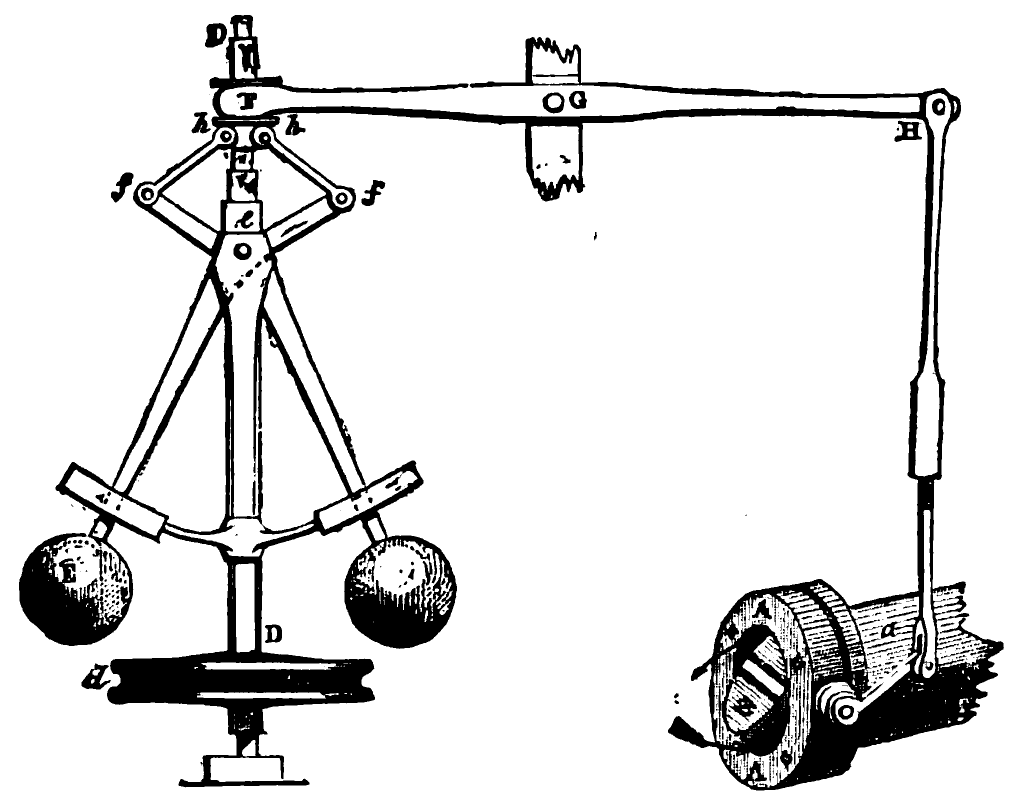
\includegraphics[width=\columnwidth]{img/Centrifugal_governor.png}%
\caption[Centrifugal governor with steam valve.]{Centrifugal governor with steam
valve. Image from \citenum{Routledge:1900:Discoveries}.}
\label{fig:centrifugal-governor}
\end{marginfigure}

\margincite{Routledge:1900:Discoveries}

\lettrine{F}{eedback control} is one of the key enabling technologies of our
time. It is hidden in many devices and appliances without most users even
noticing. The use of feedback controllers dates back to the ancient Greece,
where they were used to control water-based clocks.\ \cite[\ts
II.1]{Mayr:1970:Origins}\iss In the modern world, one of the first uses of
feedback controllers were centrifugal governors \cite{Maxwell:1867:Governors}
(Figure~\ref{fig:centrifugal-governor}) to control steam engines---sparking
the industrial revolution. Since then, feedback controllers have found their
way into our lives and we are using them every day.

A typical example is electronic stability control (ESC) in modern cars,
where the steering angle is constantly measured as a proxy to the driver's
steering intention. Also the turn rate of the car is measured with a gyroscope.
In the case of fading tire grip, the measured turn rate deviates from the
driver's intention. This discrepancy is picked up by the controller and then fed
back as control inputs in the form of brake signals for the individual wheels.
This way the car stays safely on the road, while without feedback control it
would have departed from the road.

While there exist simple model-free feedback methods to compensate deviations
from the desired value, many advanced methods require a mathematical model of
the controlled system. The model predicts the state evolution of the system and
can be used to either synthesize the feedback law or to calculate the feedback
signal in each time step. Model-based control usually requires less tuning and
can have advanced features like lookahead for reference tracking. Since we want
to make use of such features, the controllers in this thesis are all
model-based.

The classic way of doing model identification is physical modeling, e.g.,
Newton's laws can be used to deduce the mathematical equations of motion of
mechanical systems. If physical modeling is not possible, either due to the lack
of knowledge about the system, or because precise enough measurements can not be
made, \emph{system identification}~\cite{Ljung:1999:System} is often used to
find an approximation to the dynamics.

For some applications, building a controller a priori is not viable. The
systems in question might not be known beforehand or can be subject to changes
in the dynamics. In these cases, offline system identification can lead to bad
\margincite{Kumar.Varaiya:1986:Stochastic}%
system performance or may not be able to achieve the desired controller
requirements. \emph{Adaptive control}~\citenum{Kumar.Varaiya:1986:Stochastic}
offers the possibility to create controllers that are able to adapt to unknown
plants, changing plant dynamics, or unknown environments. Adaptivity means that
the control system needs a way of learning about the relevant dynamics of the
plant or the environment.

\subsection*{Disturbance Forecasting}

For many applications, controllers are built for feedback-based disturbance
rejection, which means that the effect of outside disturbances is kept small by
using the measured tracking error. However, sometimes feedback-based
disturbance rejection is not fast enough due to high performance demand or slow
measurement processes. In such cases it can help to incorporate a prediction of
the disturbance to eliminate parts of the error introduced by the disturbance in
advance.

General time-series forecasting is a challenging topic, but it gets more
manageable if the disturbance in question is of periodic nature---for example
when the origin of the disturbance is tied to the day-night-cycle or periodic
motions. In such cases, the use of periodic models to predict the disturbances
can considerably increase predictive performance and, thus, make the use of
disturbance forecasting much more available.

\subsection*{Active Identification}

Most adaptive control methods only learn in a passive manner. The available
information is used, but it is not attempted to invest control energy for
exploration or identification. In episodic settings, where the control system
executes the same task multiple times, this is often sufficient. However, for
non-episodic problems---the control of a single trial---active exploration is
an important aspect. When a system never runs twice under the same conditions,
it is crucial not only to use the available information in the best possible
way, but also to actuate the system such that the relevant information is
generated. This simultaneous identification and control is the realm of
\emph{dual control}~\cite{Wittenmark:1995:Adaptive}.

The key to differentiate between these methods is the time at which the
information is acquired. In system identification, the data is collected
upfront, before the controller is used on the plant. This also means that the
controller is not updated online. An adaptive controller is learning
``on-the-fly'', while the system is running. It collects data and updates the
internal model regularly. A dual control system goes one step further and uses
reasoning about the learning process itself to find the optimal actions. This
means that a dual controller incorporates the predicted future information
acquisition into the decision process.

\section*{Outline}

Part~\ref{par:prelimininaries} introduces the relevant mathematical background.
Gaussian process regression (Chapter~\ref{ch:gaussian-processes}) is used to
model system dynamics and external error sources. Model predictive control
(Chapter~\ref{ch:discrete-time-optimal-control}) is a well-suited control
framework for incorporating predictions into the control system. We also give
an overview on the field of adaptive control
(Chapter~\ref{ch:adaptive-control}).

Part~\ref{par:predictive-disturbance-control} shows how quasiperiodic Gaussian
process models can be used to enhance control performance. The general concept
of quasiperiodic disturbance forecasting in combination with reference tracking
model predictive control is introduced
(Chapter~\ref{ch:periodic-error-correction}) and subsequently applied to an
experimental problem in astronomical imaging: the periodic error correction in
telescope guiding (Chapter~\ref{ch:predictive-error-correction-for-telescopes}).
Based on this work, we developed software to use the periodic error correction
feature in an open source telescope guiding system
(Chapter~\ref{ch:software-implementation-phd-guiding}).

Part~\ref{par:dual-control} is concerned with the concept and application of
dual control to nonlinear systems. We first give a general overview of the dual
control literature and a classic algorithm
(Chapter~\ref{ch:introduction-to-dual-control}) which is then extended
to modern nonlinear regression techniques
(Chapter~\ref{ch:nonlinear-extensions-to-dual-control}). We further extend this
nonlinear framework to constrained systems with linear cost structure
and show a potential application to building control
(Chapter~\ref{ch:dual-control-for-buildings}).

Chapter~\ref{ch:conclusions} gives a concise summary of the work
presented in this thesis and concludes with an outlook on future research
directions.

\section*{Publications}

{\setlength{\parindent}{0pt}

Parts of the work in this thesis were done in collaboration with colleagues
and are based on the following publications:

\vspace{5mm}

Chapters~\ref{ch:periodic-error-correction} and
\ref{ch:predictive-error-correction-for-telescopes} are based on the
following journal publication:

\printpublication{Klenske.ea:2016:Gaussian}

A conference version was published in:

\printpublication{Klenske.Zeilinger.ea:2013:Nonparametric}

Chapters~\ref{ch:introduction-to-dual-control} and
\ref{ch:nonlinear-extensions-to-dual-control}, as well as
Section~\ref{sec:sparse-spectrum-approximation}, are based on the following
journal publication:

\printpublication{Klenske.Hennig:2015:Dual}

Chapter~\ref{ch:dual-control-for-buildings} is based on the following conference
publication:

\printpublication{Klenske.Hennig.ea:2016:Approximate}
}


\cleardoublepage
\phantomsection
\part{Preliminaries}\label{par:prelimininaries}

\chapter{Gaussian Process Regression}
\label{ch:gaussian-processes}

\lettrine{R}{egression} is the task of learning a functional relationship
between input and output variables from potentially noisy observations.
Regression problems are an important part of learning methods in control theory
and applications. For example, regression can be used to infer state transition
functions of dynamical systems from noisy measurements of the states. These
learned dynamics can then be used to synthesize controllers or to predict
the state evolution.

Classically in system modeling and automatic control, parametric models are
used to describe the equations of motion derived from first
principles\footnote{For example, in mechanical systems the first principles are
Newton's equations of motion.}. The parameters in such models are the physical
properties that can be measured: mass, length, etc. If possible, this is the
ideal case, but often it is difficult to describe all relevant effects a
priori. Since many systems are complex, it is challenging to come up with
perfect parametric models for them and, thus, more flexible models that can
infer unforeseen functional relationships can offer substantial benefits.

\begin{marginfigure}
\setlength\figurewidth{\columnwidth}%
\setlength\figureheight{0.618\figurewidth}%
  \inputTikZ{gauss_1d}%
  \caption[One-dimensional Gaussian distribution.]{One-dimensional Gaussian
distribution (\ref*{p:g1d}). The mean (\ref*{p:g1d-m}) and the bands of one
(\ref*{p:g1d-1sd}) and two standard deviations (\ref*{p:g1d-2sd}) are
highlighted.\vspace{\baselineskip}}
  \label{fig:1d-gauss}
\end{marginfigure}

When using flexible models, the problem of overfitting quickly arises, where
even non-effects like noise are fitted, leading to poor generalization. One way
to mitigate overfitting is to use a probabilistic prior on the function space.
Adding a prior effectively regularizes the regression problem and brings about a
global solution. A Gaussian prior on the function space is called a
\emph{Gaussian process} (GP).

\subsubsection{A Gaussian Distribution over Functions}

The well-known one-dimensional Gaussian (or \emph{normal}) distribution is shown
in Figure~\ref{fig:1d-gauss}. The Gaussian distribution is defined by two
parameters: the mean, which defines the average value, and the variance, which
defines the breadth of the distribution.

\begin{marginfigure}
\setlength\figurewidth{\columnwidth}%
\setlength\figureheight{\figurewidth}%
  \inputTikZ{gauss_2d}%
  \caption[Two-dimensional Gaussian distribution.]{Two-dimensional Gaussian
distribution. The mean (~\ref*{p:g2d-m}~) and the area of one (\ref*{p:g2d-1sd})
and two standard deviations (\ref*{p:g2d-2sd}) are shown.}
  \label{fig:2d-gauss}
\end{marginfigure}

The Gaussian distribution easily extends to the multivariate case, where we now
have a mean \emph{vector} and a \emph{co}variance \emph{matrix} defining the
distribution. The role of the mean remains the same, but since we now have
multiple variables, we not only have to define the breadth of the distribution,
but also the coupling between variables, the correlation. Breadth and shape of
the distribution are defined by the covariance matrix, where the off-diagonal
terms define the coupling between variables. Figure~\ref{fig:2d-gauss} shows a
two-dimensional Gaussian distribution.

Analogously to the extension to multiple dimensions, we can extend this notion
to entire functions. Instead of a mean vector we now have a mean
\emph{function} and instead of a covariance matrix we have a covariance
\emph{function} that defines the correlation between function values at
different inputs. The extension of the Gaussian distribution to functions is
called Gaussian process, an example is shown in Figure~\ref{fig:gauss-proc}.

\begin{marginfigure}
\setlength\figurewidth{\columnwidth}%
\setlength\figureheight{0.618\figurewidth}%
  \inputTikZ{gauss_proc}%
  \caption[Gaussian process prior.]{Gaussian process prior. Shown are the
mean (\ref*{plt:gp-pri-mean}), two standard deviations (\ref*{plt:gp-pri-var})
and three samples (\ref*{plt:gp-pri-sample}).}
  \label{fig:gauss-proc}
\end{marginfigure}

\section{Model and Notation}

A regression task is to infer a function $f(x)$ from measurements $y$ at
locations $x$. Usually the measurements are corrupted by Gaussian noise:
\begin{equation}
  y = f(x) + \gamma, \qqqq \gamma \sim \N(0,\sigma^2),
\end{equation}
where $\N$ is a Gaussian (normal) distribution.

For notational simplicity, this chapter only covers the scalar case of Gaussian
processes. In the case of a vector-valued function $f$, one GP is trained for
every dimension. For our purposes, a Gaussian process $\GP(f;m,\k)$ is an
infinite-dimensional probability distribution over the space of real-valued
\emph{functions} $f:\Re\to\Re$, such that every finite, $N$-dimensional linear
restriction to function \emph{values} $f(\mathbf{x})\in \Re^N$ (measurements)
at locations $\mathbf{x}\in\Re^N$ (measurement locations) is an $N$-variate
Gaussian distribution $\N(f(\mathbf{x}); m(\mathbf{x}),
\k(\mathbf{x},\mathbf{x}))$. It is parametrized by a mean function
$m(\mathbf{x}):\Re^N\to\Re^N$, and a covariance function
$\k(\mathbf{x},\mathbf{x}):\Re^N \times \Re^N\to \Re^{N\times N}$. The mean has
a relatively straightforward role; it simply shifts predictions. The covariance
function's responsibility is more intricate. It can be interpreted as a
similarity measure over function values, expressed in terms of the inputs, and
controls the shape of the Gaussian process belief in the space of functions. It
has to be chosen such that, for any $\mathbf{x}\in\Re^N$, the matrix
$\k(\mathbf{x},\mathbf{x}) \in \Re^{N\times N}$, also known as the
\emph{kernel} matrix, is positive semidefinite.

As common in the Gaussian process literature, without loss of generality, we
assume the mean function $m$ to be zero to simplify notation. Note that this
does not imply that only zero-mean Gaussian processes should be considered for
practical applications. Rather, the choice of mean function should be part of
the modeling considerations.

\section{Inference in Gaussian Processes}

The main inference machinery in the GP regression framework is Bayes' rule
\begin{equation*}
  \text{posterior} = \frac{\text{likelihood} \times
\text{prior}}{\text{evidence}},
\qq
  p(\M|\D) = \frac{p(\D|\M) \times p(\M)}{p(\D)}
\end{equation*}
where $p$ is a probability density function, $\D$ stands for the data and $\M$
for the model. When the prior is a Gaussian process and the likelihood is
Gaussian, the posterior is again a Gaussian process. The mean and covariance
function of the posterior can be calculated in closed form with linear algebra
calculations.

Even if the Gaussian process $\GP(f;m,k)$ is an infinite-dimensional object with
mean function $m$ and covariance function $k$, we can reason about any finite
amount of data points $\mathbf{x}=[x_1, \dots, x_N]$ and prediction point $x$
by evaluating the mean and covariance function at those locations only. This
amounts to the application of the marginalization rule of Gaussian algebra
\cite[\ts2.3]{Bishop:2006:Pattern} and results in a multivariate Gaussian
distribution. Stacking the predictive value $y$ and the vector of noise-free
function evaluations $\mathbf{y}=[y_1; \dots; y_N]$ into one vector results in
the following joint distribution
\begin{equation}
  \label{eq:joint-gaussian}
  \begin{bmatrix}y\\\mathbf{y}\end{bmatrix}
  \sim \N\left(\begin{bmatrix}0\\0\end{bmatrix},
  \begin{bmatrix}\k_{xx} & \k_{x\mathbf{x}} \\
    \k_{\mathbf{x}x} & \k_{\mathbf{x}\mathbf{x}} \end{bmatrix} \right),
\end{equation}
where we have introduced the shorthand notation $\k_{\cdot\cdot} =
\k(\cdot,\cdot)$.

\begin{marginfigure}[28mm]
\setlength\figurewidth{\columnwidth}%
\setlength\figureheight{0.618\figurewidth}%
  \inputTikZ{gauss_proc_post}%
  \caption[Gaussian process posterior after two noise-free observations.]
  {Gaussian process posterior after two noise-free observations.
Shown are the mean (\ref*{plt:gp-post-mean}), two standard deviations
(\ref*{plt:gp-post-var}) and three samples (\ref*{plt:gp-post-sample}).}
  \label{fig:gauss-proc-post}
\end{marginfigure}

Since we have measured $\mathbf{y}$, but not $y$, we apply the conditioning
rule \citenum[\ts2.3]{Bishop:2006:Pattern} of Gaussian algebra to obtain
\begin{equation}
  \label{eq:gaussian-conditioning}
  y \sim \N\left( \k_{x\mathbf{x}} K\inv \mathbf{y},
  \k_{xx} - \k_{x\mathbf{x}} K\inv  \k_{\mathbf{x}x}
  \right),
\end{equation}
where $K=\k(\mathbf{x},\mathbf{x})$. The matrix $K$ is called the Gram matrix
(or \emph{kernel} matrix). We can write the predictive mean and predictive
covariance explicitly as
\begin{subequations}
\label{eq:gp-post}
\begin{align}
m^{|\mathbf{x},\mathbf{y}}(x) &= \k_{x\mathbf{x}} K\inv \mathbf{y}\\
k^{|\mathbf{x}}(x,x') &= \k_{xx'} - \k_{x\mathbf{x}} K\inv
\k_{\mathbf{x}x'},
\end{align}
\end{subequations}
which can easily be implemented.\footnote[][-10mm]{Note that, while
the formulation \eqref{eq:gp-post} is mathematically concise, the Cholesky
decomposition \citenum{Rasmussen.Williams:2006:Gaussian} of the Gram
matrix is usually used to carry out the calculations for increased speed and
numerical stability.}\margincite{Rasmussen.Williams:2006:Gaussian}
Figure~\ref{fig:gauss-proc-post} shows an example of a GP posterior with
noise-free observations. After conditioning on the measurements, the function
space is restricted to functions that pass through them.

So far, we only considered noise-free observations. Adding independent and
identically distributed Gaussian observation noise to the GP framework is done
simply by adding measurement noise to the Gram matrix $K$:
\begin{equation}
  \label{eq:noisy-gram-matrix}
  K_\text{noisy} = \k(\mathbf{x},\mathbf{x}) + \sigma^2 I
\end{equation}
The inference under noisy measurements results in a similar posterior, with the
difference that the posterior mean is closer to the prior, and the pointwise
posterior distribution is not as narrow as in the noise-free case.
Figure~\ref{fig:gauss-proc-post-n} shows an example of GP inference under noise.

\begin{marginfigure}[-45mm]
\setlength\figurewidth{\columnwidth}%
\setlength\figureheight{0.618\figurewidth}%
  \inputTikZ{gauss_proc_post_noise}%
  \caption[Gaussian process posterior after two noisy observations.]
  {Gaussian process posterior after two noisy observations.
Shown are the mean (\ref*{plt:gp-post-n-mean}), two standard deviations
(\ref*{plt:gp-post-n-var}) and three samples (\ref*{plt:gp-post-n-sample}).}
  \label{fig:gauss-proc-post-n}
\end{marginfigure}

\section{Sampling from Gaussian Processes}

Gaussian processes are generative models. This means that it is possible to
draw samples from the prior or posterior distribution, similar to drawing
from a Gaussian distribution. This is of two-fold importance:

First, methods that use the GP model might need samples for numerical
marginalization, when analytic integration is intractable. Instead of
calculating an expectation directly, a sum over samples can serve as
approximation
\begin{equation}
  \Exp_{f}\left[c(f)\right]= \int c(f) \GP(f;m,\k) df \approx \frac{1}{S}
\sum_{i=1}^S c(s_i),
\end{equation}
where $c(f)$ is a functional operator and $s_i$ are the samples from the GP.

Secondly, samples are a great tool for analyzing the function space defined by
the GP. It is important to note that the mean of a GP looks fundamentally
different from samples from the same process, see Figures~\ref{fig:gauss-proc}
and \ref{fig:gauss-proc-post}. This is due to the smoothing property of the
mean \cite[\ts~2.6]{Rasmussen.Williams:2006:Gaussian}. For choosing the
covariance function and its parameters\footnote[][3mm]{See Sections
\ref{sec:covariance-functions} and \ref{sec:parameter-fitting}.} it is, thus,
helpful to compare samples of the selected GP with real data to see if they
look similar. This can help in the analysis of how the chosen model fits the
data.

For finite-dimensional datasets, where the samples $s$ are vectors of function
\emph{evaluations} at locations $\mathbf{x}$, the sampling process is relatively
straightforward, since it is equivalent to sampling from a multivariate Gaussian
distribution with the covariance of the GP:
\begin{equation}
  s = L \rho,
\end{equation}
where $L$ is a matrix satisfying $LL\T = \k(\mathbf{x},\mathbf{x})$ and $\rho$
is a random Gaussian vector of appropriate size. $\k$ can be any suitable
positive semidefinite covariance function, especially also the posterior
covariance of a GP.

\section{Choosing a Covariance Function}
\label{sec:covariance-functions}

The covariance function defines how samples and predictions of the Gaussian
process look like, by shaping the underlying probability distribution in the
function space. So far, we considered the covariance function as given. But
where does it come from, and how should it be chosen?

There is an alternate way of deriving Gaussian processes, usually called the
``weight-space view'' \cite[\ts~2.1]{Rasmussen.Williams:2006:Gaussian}. We will
not reproduce the entire derivation here, but instead point out certain
aspects.

Consider general linear regression
\begin{equation}
  f(x) = w\T\Phi(x),
\end{equation}
where $w$ are weights and $\Phi(x)$ is a vector of potentially nonlinear feature
functions. The shape of the functions that can be represented by this
model is defined by the shape of the chosen feature functions.

The notion of general linear regression can be expressed in the GP framework
and can be extended to the nonparametric case with infinitely many
features.\footnote{This is usually done by reformulating, and application of the
famous ``kernel trick''
\citenum[\ts2.2]{Scholkopf.Smola:2002:Learning}.}\margincite{
Scholkopf.Smola:2002:Learning} We then obtain a covariance function (or
\emph{kernel}) that is defined by the feature functions that we have chosen in
the first place. This means that, by the choice of covariance function, we can
choose the shape of the functions that can be represented by the Gaussian
process.

Theoretically, every positive semidefinite kernel can be used as covariance
function for a Gaussian process. However, for this thesis, we only consider
stationary covariance functions, for which the covariance depends on the
distance $r=|x-x'|$ of the inputs and not on the location itself.

\subsection{Output Correlation}

The covariance function of a Gaussian process defines a mapping from the
distance $r$ in input space to correlation in output space. For radial basis
functions, for example, this means that the function values of two points that
are close in input space are correlated to a higher degree than the function
values of points that are far away in input space.
Figure~\ref{fig:gauss-output-corr} visualizes this.

\begin{figure}
\setlength\figurewidth{\columnwidth}%
\setlength\figureheight{0.618\figurewidth}%
  \resizebox{\columnwidth}{!}{\inputTikZ{gauss_output_corr}}%
  \caption[Correlation of different points in output space.]{Correlation
of different points in output space for a radial basis function.
{\bfseries Top:} GP with mean
(\ref*{plt:gp-pri-mean}), two standard deviations
(\ref*{plt:gp-pri-var}) and three samples (\ref*{plt:gp-pri-sample}). {\bfseries
Middle:} Correlation function (\ref*{p:corr-cov}) for the
reference location (\ref*{p:corr-ref}) and evaluation locations
(\ref*{p:corr-eval}). {\bfseries Bottom:} Two-dimensional Gaussian
distributions between the reference location and the different evaluation
locations, shown as areas for 1 and 2 standard deviations
(\ref*{p:corr-1sd}/\ref*{p:corr-2sd}).}
  \label{fig:gauss-output-corr}
\end{figure}

This correlation between function values is responsible for the overall shape
of samples of the GP. If points that are relatively close in input space have a
high correlation, this means that there is not much variability in the sampled
functions, and the inputs have to move further away to allow for significant
changes in the function values. If the correlation between nearby points is
low, this allows for high variability within shorter distance: The functions
are more flexible.

\subsection{Examples of Covariance Functions}

There are many different covariance functions to choose from. In this section
we only provide those which are relevant for this thesis.

\subsubsection{Square Exponential Covariance Function}

\begin{marginfigure}
\setlength\figurewidth{\columnwidth}%
\setlength\figureheight{0.618\figurewidth}%
  \inputTikZ{kernel_se}%
  \caption{Square exponential covariance function.}
  \label{fig:kern-se}
\end{marginfigure}

One important covariance function is the square
exponential\footnote[][3mm]{Also known as ``squared exponential'',
``exponentiated quadratic'', ``radial basis function'' (RBF) or ``Gaussian''
covariance function.}
\begin{equation}
  \label{eq:cov-se}
  \k_\mathsc{se}(x, x'; \theta, \ell) = \theta^2
  \exp\left(-\frac{|x-x'|^2}{2\ell^2}\right),
\end{equation}
where $\theta^2$ is the signal variance and $\ell$ the length scale parameter.
Using this covariance function is equivalent to infinite-dimensional Gaussian
feature regression. It is differentiable and integrable and therefore compatible
to many use-cases. The shape of the square exponential covariance function is
shown in Figure~\ref{fig:kern-se}.

\subsubsection{Periodic Covariance Function}
\label{sec:periodic-covariance}

\begin{marginfigure}
\setlength\figurewidth{\columnwidth}%
\setlength\figureheight{0.618\figurewidth}%
  \inputTikZ{kernel_per}%
  \caption{Periodic covariance function.}
  \label{fig:kern-per}
\end{marginfigure}

Much more specific is the periodic covariance function
\cite{MacKay:1998:Introduction}
\begin{equation}
  \label{eq:cov-per}
  \k_\mathsc{p}(x,x';\theta,\ell,\lambda) = \theta^2
  \exp\left(-\frac{2\sin^2\left(\frac{\pi}{\lambda}
  (x-x')\right)}{\ell^2}\right),
\end{equation}
where $\theta^2$ and $\ell$ are similar parameters as above, and $\lambda$ is
the period length. This periodic covariance is essentially a square exponential
covariance where the inputs are warped through a sine. A GP with this covariance
function can only represent periodic functions with a specified period length
$\lambda$. This might seem restrictive, but it can be valuable because it is
much more data efficient than other covariances and has better extrapolation
performance because stronger assumptions on the underlying function space are
made. The shape of the periodic covariance function is shown in
Figure~\ref{fig:kern-per}.

\subsection{Combined Covariance Functions}

In practice, the functions we want to learn are often mixtures of different
signals and it is hard to find a covariance function that suits all of
them simultaneously. Instead of trying to fit all components with a single
covariance function, which usually leads to poor data efficiency and/or
predictive performance, the Gaussian process framework is flexible enough to
allow for combinations of covariance functions.

In practice, combined covariance functions are obtained by element-wise
addition or multiplication of the kernel matrices:
\begin{equation}
  \k_\mathsc{c}(\mathbf{x},\mathbf{x}) = k_1(\mathbf{x},\mathbf{x}) +
k_2(\mathbf{x},\mathbf{x})
\end{equation}
or
\begin{equation}
  \k_\mathsc{c}(\mathbf{x},\mathbf{x}) = k_1(\mathbf{x},\mathbf{x}) \odot
k_2(\mathbf{x},\mathbf{x}),
\end{equation}
where $\k_\mathsc{c}$ stands for the kernel combination and $\k_1$,
$\k_2$ are the individual kernels. The meaning of the additive kernel is
relatively simple: It adds two different functions on top of each
other.~\cite[\ts4.2]{Rasmussen.Williams:2006:Gaussian}\iss One example for a GP
with additive covariance structure is shown in
Figure~\ref{fig:kernel-combination}.

 \begin{figure}
  \setlength\figurewidth{0.507\columnwidth}%
  \setlength\figureheight{0.618\figurewidth}%
  \inputTikZ{gauss_proc_comb_pri}\inputTikZ{gauss_proc_comb_post}%
  \caption[Gaussian process prior and posterior for an additive
covariance.]{Gaussian process prior (left) and posterior (right) for an
additive covariance. The covariance function is combined from a square
exponential and a periodic covariance. Shown are the mean
(\ref*{plt:gp-comb-pri-mean}), two standard deviations
(\ref*{plt:gp-comb-pri-var}) and one sample (\ref*{plt:gp-comb-pri-sample})
each.}
  \label{fig:kernel-combination}
\end{figure}

The effect of multiplying kernels is more intricate. While it can be shown that
element-wise multiplications still retain the positive-definiteness of the
resulting matrices \cite{Schur:1911:Bemerkungen}, it is harder to grasp what
this means for the function. In a way, the multiplication acts similarly to a
logical \texttt{and}, so that there is a high correlation between points that
have a high correlation under \emph{both} covariance functions.

\subsubsection{Output Projections}
\label{sec:output-projections}

When inference is done with a covariance combination, it is also possible to
split the prediction to the different parts for additional interpretation
possibilities or for the subsequent use in other algorithms. This is done with
the Gaussian algebra of Equations~\eqref{eq:joint-gaussian} and
\eqref{eq:gaussian-conditioning} by conditioning the prediction on the kernels
that we are interested in.

\pagebreak[4]

If, for example, the prediction should be done only for kernel 1, the
resulting predictive posterior amounts to \cite{Duvenaud:2014:Automatic}
\begin{subequations}
\label{eq:output-projection}
\begin{align}
m^{|\mathbf{x},\mathbf{y}}_1(x) &= \k_1(x,\mathbf{x}) K_{\mathsc{c}}\inv
\mathbf{y}\\
k^{|\mathbf{x}}_1(x,x') &= \k_1(x,x') -\k_1(x,\mathbf{x})
K_{\mathsc{c}}\inv
  \k_1(\mathbf{x},x').
\end{align}
\end{subequations}
where $K_\mathsc{c}$ is the Gram matrix for a combined kernel and $\k_1$ is
the kernel function for only one of the kernels. The effect of this conditioning
of the posterior is shown in Figure~\ref{fig:different-output-projections},
using the same kernel combination as in Figure~\ref{fig:kernel-combination}.

 \begin{figure}
  \setlength\figurewidth{0.507\columnwidth}%
  \setlength\figureheight{0.618\figurewidth}%
  \inputTikZ{gauss_proc_comb_proj1}\inputTikZ{gauss_proc_comb_proj2}%
  \caption[Comparing different output projections from a combined
covariance.]{Comparing different output projections from a combined
covariance. The Gaussian conditioning shows the periodic component (left) and
the square exponential component (right) respectively. Shown are the mean
(\ref*{plt:gp-comb-proj1-mean}/\ref*{plt:gp-comb-proj2-mean}), two
standard deviations (\ref*{plt:gp-comb-proj1-var}/\ref*{plt:gp-comb-proj2-var})
and one sample
(\ref*{plt:gp-comb-proj1-sample}/\ref*{plt:gp-comb-proj2-sample}) each.}
  \label{fig:different-output-projections}
\end{figure}

\vspace{-\baselineskip}
\section{Setting the Kernel Parameters}
\label{sec:parameter-fitting}

Most covariance functions have parameters, like the signal variance $\theta^2$
or the length scale $\ell$ in Equation~\eqref{eq:cov-se}. These parameters are
usually called \emph{hyper}para\-meters. The reason for this name is the idea
of a Gaussian process being an infinite-dimensional linear regression model: In
linear regression, the weights for the different features are called
parameters, and the Gaussian process has infinitely many of these
parameters.\footnote{These methods are also referred to as \emph{non}parametric
in the literature, to stress the fact that there is no \emph{finite} amount of
features to select.} To distinguish the parameters of the covariance function
from the linear regression parameters, they are called \emph{hyperparameters}.

\subsection{The Role of the Hyperparameters}

Even though covariance functions like the square exponential are
\emph{universal kernels} that can theoretically learn any function
\cite{Micchelli.Xu.ea:2006:Universal}, it is important to set the
hyperparameters correctly. Otherwise the learning can be inefficient and might
need much more data than a GP with a suitable set of
hyperparameters.~\cite{van-der-Vaart.van-Zanten:2011:Information}

\subsubsection{Output Variance}

The scale factor ($\theta^2$ in Equation~\eqref{eq:cov-se}) of the covariance
function defines the output variance of the GP, \ie the range over which
functions typically vary in value. The effect of this parameter is visualized
in Figure~\ref{fig:different-signal-variances}.

\pagebreak[4]

\begin{figure}
  \setlength\figurewidth{0.507\columnwidth}%
  \setlength\figureheight{0.618\figurewidth}%
  \inputTikZ{gauss_proc_high}\inputTikZ{gauss_proc_low}%
  \caption[Gaussian process with high/low signal variance.]{Gaussian process
with high signal variance (left) compared to one with low signal variance
(right), using a square exponential kernel. Shown are the mean
(\ref*{plt:gp-pri-mean}), two standard deviations
(\ref*{plt:gp-pri-var}) and three samples (\ref*{plt:gp-pri-sample}) each. The
higher signal variance allows for larger function values.}
  \label{fig:different-signal-variances}
\end{figure}

\subsubsection{Length Scale}

Most covariance functions have a length scale parameter ($\ell$ in
Equation~\eqref{eq:cov-se}). Often, changing the length scale parameter is
equivalent to a scaling of the input distance. This parameter defines how much
the function values can vary relative to the input distance. The effect of this
parameter is visualized in Figure~\ref{fig:different-length-scales}.

\begin{figure}
  \setlength\figurewidth{0.507\columnwidth}%
  \setlength\figureheight{0.618\figurewidth}%
  \inputTikZ{gauss_proc_long}\inputTikZ{gauss_proc_short}%
  \caption[Gaussian process with long/short length scale.]{Gaussian process
with long length scale (left) compared to one with short length scale (right),
using a square exponential kernel.
Shown are the mean (\ref*{plt:gp-pri-mean}), two standard deviations
(\ref*{plt:gp-pri-var}) and three samples (\ref*{plt:gp-pri-sample}) each. The
shorter length scale allows for more variation within the same distance in input
space.}
  \label{fig:different-length-scales}
\end{figure}

\subsubsection{Period Length}

The periodic covariance has a period length parameter ($\lambda$ in
Equation~\eqref{eq:cov-per}). This parameter defines the distance in input
space after which the function repeats itself. The effect of this parameter is
visualized in Figure~\ref{fig:different-period-length}.

\begin{figure}
  \setlength\figurewidth{0.507\columnwidth}%
  \setlength\figureheight{0.618\figurewidth}%
  \inputTikZ{gauss_proc_per_long}\inputTikZ{gauss_proc_per_short}%
  \caption[Gaussian process with long/short period length.]{Gaussian process
with long period length (left) compared to one with short period length
(right), using a periodic kernel. Shown are the mean
(\ref*{plt:gp-pri-mean}), two standard deviations
(\ref*{plt:gp-pri-var}) and one sample (\ref*{plt:gp-pri-sample}) each. The
sampled functions are perfectly periodic with the chosen period length.}
  \label{fig:different-period-length}
\end{figure}

\subsection{The Hyperparameter Likelihood}

For many applications it can be enough to choose the hyperparameters from
physical reasoning, but this is not always the case. Especially for automatic
parameter tuning it is important to assess how good the parameters fit the data.

Assume that all kernel parameters are subsumed in the parameter vector
$\boldsymbol{\eta}$. Inferring good values for $\boldsymbol{\eta}$ is important
for good modeling performance. The fundamental framework for GP inference is
provided by Bayes' theorem. The likelihood for observations $\mathbf{y}$ at
locations $\mathbf{x}$, conditioned on the parameters $\boldsymbol{\eta}$, can
be found by marginalization over the unknown function $f$, which is feasible
because both $p(\mathbf{y}|f)$ and $p(f|\boldsymbol{\eta})$ are Gaussian
distributions:
\begin{align}
  p(\mathbf{y}|\mathbf{x},\boldsymbol{\eta}) &= \int
  p(\mathbf{y}|f)p(f|\boldsymbol{\eta}) df\\
  \notag
  &= \int \N(\mathbf{y};f(\mathbf{x}),\sigma^2 I)\GP(f;0,\k(\boldsymbol{\eta}))
  df\\
  \notag &= \N(\mathbf{y};0,K(\boldsymbol{\eta})).
\end{align}

These calculations are easier to perform in log domain,
where the logarithm of the marginal likelihood is given by
\begin{equation}
\label{eq:log-likelihood}
  \log p(\mathbf{y} | \mathbf{x},\boldsymbol{\eta}) = - \frac{1}{2} \mathbf{y}\T
  K(\boldsymbol{\eta})\inv
  \mathbf{y} - \frac{1}{2} \log \left|K(\boldsymbol{\eta})\right| -\frac{N}{2}
  \log 2\pi.
\end{equation}
With this likelihood, it is easy to compare the model fit for different sets of
hyperparameters.

\subsection{Hyperparameter Optimization}
\label{sec:typeII-ML}

One way of setting the hyperparameters is to maximize the marginal likelihood
\eqref{eq:log-likelihood},
\begin{equation}
  \boldsymbol{\eta}^* = \underset{\boldsymbol{\eta}}{\argmax}
p(\mathbf{y}|\mathbf{x},\boldsymbol{\eta}).
\end{equation}
This is usually done with a gradient-based optimizer;
often quasi-Newton methods, such as the BFGS algorithm
\margincite{Nocedal.Wright:2006:Numerical}%
\citenum[\ts6.1]{Nocedal.Wright:2006:Numerical}, are used. Since the
optimization leads to the maximum likelihood (ML) solution for the
hyperparameters, it is usually called \emph{type-II maximum
likelihood}\footnote{The maximum likelihood approach is also known as
\emph{evidence maximization} in the literature.}, to distinguish it from the GP
inference itself.~\cite[\ts
5.4.1]{Rasmussen.Williams:2006:Gaussian}\iss In a way, hyperparameter
optimization can be seen as a second layer of inference on top of the
Gaussian process.

Using the ML estimate is one of the most widely studied and best understood
strategies in statistics.~\cite[\ts9.3 -- \ts9.6]{Wasserman:2010:All}\iss It is
not without weaknesses, \eg the optimization is prone to get stuck in local
minima. Some of these weaknesses are often resolved if enough data is available,
or by the use of customized optimization algorithms. Other approaches, for
example, integrating the hyperparameters over ML estimates or cross validation,
have been examined in the past and found to perform worse than the above type-II
maximum likelihood approach in practice, see, \eg \cite{MacKay:1999:Comparison}.

\subsection{Priors on the Hyperparameters}
\label{sec:typeII-MAP}

In order to make the method more robust, it can be beneficial to introduce
priors on the parameters. For the strictly positive parameters
$\boldsymbol{\eta}$, gamma priors
\cite[\ts8.3]{Barber:2011:Bayesian} are a classic choice:
\begin{equation}
  p(\boldsymbol{\eta}| \boldsymbol{\kappa},\boldsymbol{\tau}) = \prod_i
\frac{\boldsymbol{\eta}_i
^{\kappa_i-1}\exp(-\frac{\boldsymbol{\eta}_i}{\tau_i})}{\Gamma(\kappa_i)\tau_i
^{\kappa_i}},
\end{equation}
where $\kappa_i$ and $\tau_i$ are tuning-parameters\footnote{Sometimes also
referred to as hyper-hyperparameters.}, and $\Gamma$ is the gamma function.

Again, the maximization is easier to perform in log domain, in which the effect
of the prior is additive, leading to the following optimization problem:
\begin{multline}
\label{eq:maximum-posterior}
  \boldsymbol{\eta}^* = \underset{\boldsymbol{\eta}}{\argmax}
p(\boldsymbol{\eta}|\mathbf{y},\mathbf{x}) =
\underset{\boldsymbol{\eta}}{\argmax}
p(\mathbf{y}|\mathbf{x},\boldsymbol{\eta})p(\boldsymbol{\eta}) \\
  = \underset{\boldsymbol{\eta}}{\argmax} (\log
p(\mathbf{y}|\mathbf{x},\boldsymbol{\eta}) + \log p(\boldsymbol{\eta}) ).
\end{multline}
In \eqref{eq:maximum-posterior}, the prior effectively turns into a
regularizer, simplifying optimization and avoiding degeneracy. The additional
computational cost is negligible compared to the matrix inversion needed for
(\ref{eq:log-likelihood}).

\section{Numerical Effort and Approximations}

Gaussian processes are generally considered to be a relatively expensive
method. This is due to the matrix inversion and determinant calculation in
Equation~\eqref{eq:gaussian-conditioning} which both have
(na\"ive\footnote{Sometimes, lower complexity numbers are reported for using the
Strassen algorithm \citenum{Strassen:1969:Gaussian} and further improvements,
but they are rarely implemented in
practice.}\margincite{Strassen:1969:Gaussian}) asymptotic complexity of
$\O(N^3)$ in the number of samples $N$. For large amounts of training data, this
can be prohibitive.

In the light of using GPs for applications in automatic control, there is
another point to consider: It is rarely, if ever, acceptable to have growing
inference cost over time. Control algorithms should run reliably fast and
therefore have almost constant runtime for both the inference and the control
part.

There are many different ways of dealing with the numerical complexity of
Gaussian processes, see Chapter 8 of the textbook by
\textcite{Rasmussen.Williams:2006:Gaussian} for an overview. In the following,
we review two methods that will be used in subsequent chapters of this
work.

\subsection{Subset-of-Data Approximation}
\label{sec:subset-of-data}

One of the simplest and most efficient approximation methods is the
Subset-of-Data (SD\footnote{In the literature also abbreviated as ``SoD''.})
method. The idea is to reduce the number $N$ of available data points by
considering only a smaller subset of $M$ data points with $M \ll N$. Since $M$
can be chosen in advance, the runtime of the algorithm is known and remains
constant.

Changing the set of data points does not change the inference algorithm at all;
therefore, this method can be implemented quickly and efficiently. Of course,
the considered data points need to be chosen at runtime. Ideally the selection
should be done according to how informative a data point is, but this
optimization can be demanding, too. Hence, usually approximative methods are
used. For example, depending on the expected distribution of data points in the
dataset, the used data can be randomly sampled or selected by optimization of
some criterion, \eg a differential entropy score
\cite{Lawrence.ea:2003:Fast}.

\subsection{Sparse Spectrum Approximation}
\label{sec:sparse-spectrum-approximation}

By Mercer's theorem \cite[\ts3.a]{Konig:1986:Eigenvalue}, the kernel can be
decomposed into a converging series over eigenfunctions $\phi(x)$, as
\begin{equation}
  \label{eq:mercer}
  \k(x,x') = \sum_{l=1} ^\infty \lambda_l \phi _l(x) \phi_l ^*
(x'),
\end{equation}
where $\phi_l$ are functions that are orthonormal relative to some measure $\mu$
(the precise choice of which is irrelevant for the time being), with the
property
\begin{equation}
  \int \k(x,x') \phi_l(x') d\mu(x') = \lambda_l \phi_l(x).
\end{equation}

In this sense, Gaussian process regression can be seen as
``infinite-dimensional'' Bayesian linear regression, where the infinite inner
product \eqref{eq:mercer} is tractable because of the kernel trick
\cite[\ts2.2]{Scholkopf.Smola:2002:Learning}.

Using the kernel formulation comes at the cost of a growing Gram matrix and,
thus, rising inference cost, and is rarely acceptable for practical control
applications. Therefore, it is often necessary to project the GP belief onto a
finite representation, replacing the infinite sum in Equation~(\ref{eq:mercer})
with a finite inner product of a low-dimensional explicit feature map $\Phi(x)$
\begin{equation}
  \k(x,x') \approx \Phi(x)\T\Lambda\Phi(x'),
\end{equation}
where $\Lambda$ is a diagonal eigenvalue matrix.
This bounds the computational cost of the inference \eqref{eq:gp-post},
because the more efficient formulae of general linear regression can be used
\begin{subequations}
\label{eq:featue-post}
\begin{align}
  m^{|\mathbf{x},\mathbf{y}}(x) &= \frac{1}{\sigma^2}\Phi(x)\T
A\inv\Phi(\mathbf{x})
\mathbf{y}\\
  k^{|\mathbf{x}}(x,x') &= \Phi(x)\T A\inv\Phi(x),
\end{align}
\end{subequations}
where $A=\sigma^{-2}\Phi(\mathbf{x})\Phi(\mathbf{x})\T +\Lambda^{-1}$.

We define the feature map $\Phi$ that projects the inputs onto a pre-defined
finite basis of functions, drawn from the eigenspectrum of the kernel with
respect to the Lebesgue measure. Similar approaches have been recently proposed
in the literature \cite{Lazaro.ea:2010:Sparse}, \cite{Rahimi.Recht:2008:Random}.
The following provides a short, self-contained introduction:

By Bochner's theorem \cite[\ts2.5]{Stein:1999:Interpolation}, the covariance
function $k(r)$ (with $r=|x-x'|$) of a stationary mean-square continuous random
process can be represented as the Fourier transform of a positive finite measure
and, if that measure has a density $S(s)$, as the Fourier dual of $S$:
\begin{equation}
  \k(r) = \int\limits_{-\infty}^\infty S(s)e^{2\pi \imath s r} ds,
\end{equation}
where $\imath$ is the imaginary unit.
This means that the eigenfunctions of the kernel are trigonometric functions,
and stationary covariance functions, like the commonly used square exponential
kernel \eqref{eq:cov-se}, can be approximated by cosine basis functions as
\begin{equation}
  \k(x,x') \approx \tilde \k(x,x') =
\frac{\theta^2}{F}\sum_{i=1}^{F} \cos(\omega_{i} |x-x'|),
\end{equation}
where $F$ is the number of features, and the frequencies $\omega_i$ of the
feature functions can be sampled from the power spectrum of the
process.\footnote{For example, the Latin hypercube sampling technique
\citenum{McKay.Beckman.ea:1979:Comparison} can be
used.}\margincite{McKay.Beckman.ea:1979:Comparison} An example of such kernel
approximation is shown in Figure~\ref{fig:kernel-approximation}. With increasing
number of features, the approximation can be chosen as close to the true
covariance function as needed, while keeping the number of features in a range
that is still feasible within the time constraints of the control algorithm.

\begin{figure*}
  \setlength\figureheight{0.5\textwidth}%
  \setlength\figurewidth{\textwidth}%
  \footnotesize%
  \resizebox{\columnwidth}{!}{\inputTikZ{kernel_comparison}}%
  \caption[Comparison of a finite kernel approximation to the full
kernel.]{Comparison of a finite kernel approximation to the full kernel. Prior
(left), posterior (middle) and kernel function (right) of both the full kernel
function (top row) and the approximate kernel (bottom row). Shown are the mean
(\ref*{p:full-mean}/\ref*{p:approx-mean}), two standard deviations
(\ref*{p:full-std}/\ref*{p:approx-std}) and three samples each
(\ref*{p:full-sample}/\ref*{p:approx-sample})}
  \label{fig:kernel-approximation}
\end{figure*}

\section{Extensions}

The Gaussian process framework is powerful and has many useful features
and extensions. Two further concepts are important for this thesis and will
thus be presented here.

\subsection{Heteroscedastic Noise}
\label{sec:heteroscedastic-noise}

Usually noise is assumed uniform for all measurements (homoscedastic), but this
may not be satisfied in practice. Not all measurement processes have constant
noise level, therefore it can be useful to consider heteroscedastic noise
instead, allowing for variable noise variance.

The additive noise matrix in Equation~\eqref{eq:noisy-gram-matrix} can also be
given in the form of a diagonal matrix
\begin{equation}
  K_\text{noisy} = k(\mathbf{x},\mathbf{x}) +
  \begin{pmatrix}\sigma^2_1 &&\\&\ddots&\\&&\sigma^2_N\end{pmatrix},
\end{equation}
where $\sigma^2_i$ for $i=\{1\dots N\}$ is the noise variance for the $i$-th
measurement. This way a sensor or measurement method with variable noise level
can be modeled accurately within the Gaussian process framework.

\subsection{Explicit Feature Functions}
\label{sec:explicit-feature-functions}

Since Gaussian processes are related to general linear regression, it is
possible to combine both methods. This is useful if certain parts of a
regression problem can be modeled as parametric features and other parts can
not. Even though a GP can potentially learn everything, it is much more
efficient to model as much as possible in the form of parametric features and
train a more general GP for the remainder only.

An additive combination of general linear regression and Gaussian process can be
modeled as
\begin{equation}
  g(x) = \beta\T \psi(x) + f(x),
\end{equation}
where $\beta\sim\N(b,B)$ is a parameter vector, $\psi$ is a set of parametric
feature functions and $f(x)\sim \GP(0,k_f)$.

A numerically stable way of formulating the predictive mean and covariance is
\cite[\ts2.7]{Rasmussen.Williams:2006:Gaussian}
\begin{subequations}
\label{eq:joint-model}
\begin{align}
   m_g^{|\mathbf{x},\mathbf{y}}(x) &= m_f^{|\mathbf{x},\mathbf{y}}(x) + \bar
\beta  \T R(x)\\
   k_g^{|\mathbf{x}}(x,x') &= k_f^{|\mathbf{x}}(x,x') + R(x)\T\left(B\inv +
  \Psi K\inv \Psi\T\right)\inv R(x'),
\end{align}
\end{subequations}
where the feature matrix $\Psi$ collects the feature vectors $\psi(\mathbf{x})$
for all
data points, $\bar \beta = (B\inv + \Psi K\inv \Psi\T)\inv (\Psi K\inv
\mathbf{y} + B\inv b)$, and $R(x) = \psi(x) - \Psi K\inv
\k_f(\mathbf{x},x)$. These calculations represent the inference in the joint
model,
combining general linear regression with a Gaussian process. If the prior on
the parametric part of the model should be uninformative, one can obtain the
limit case by letting $B\inv \to 0$, which is possible in the formulation of
Equation~\eqref{eq:joint-model}.

\renewcommand{\u}{\mathbf{u}}

\chapter{Discrete-Time Optimal Control}
\label{ch:discrete-time-optimal-control}

\lettrine{M}{odel-based} optimal control is successfully used in many
control systems and poses a prerequisite for this thesis. Since the topic is
rather broad, we only cover the topics relevant for this thesis.

We briefly introduce linear time-invariant (LTI) systems and the concepts of
stability and controllability (Section~\ref{sec:lti-systems}). For LTI systems,
we describe different types of model-based optimal controllers: Dynamic
programming based optimal control (Section~\ref{sec:dynamic-programming}) and
model predictive control by constrained optimization
(Section~\ref{sec:model-predictive-control}). We introduce the concept of
receding horizon control (Section~\ref{sec:receding-horizon}) and describe some
important extensions of discrete-time optimal control
(Section~\ref{sec:doc-extensions}).

\section{Linear Time-Invariant Systems}
\label{sec:lti-systems}

Linear time-invariant (LTI) systems are often used in model-based control due
to their advantageous computational properties. Even though most systems
are not linear, often a linear approximation to a nonlinear system offers good
performance in the vicinity of the operating point.
\cite[\ts2.7]{Ogata:2010:Modern}

For this chapter, we use the common discrete-time LTI system
\begin{equation}
  \label{eq:lti-system}
  x(t_{k+1}) = A x(t_k) + B u(t_k),\quad k\in\mathbb{N},
\end{equation}
where $t_k\in\Re$ denotes the $k$-th time instant relative to the
sampling time $\Delta t$, $x\in\Re^{n_x}$ is the state, $A\in\Re^{n_x\times
n_x}$ is the discrete-time state-transition matrix and $B\in\Re^{n_x\times n_u}$
is the discrete-time input matrix.

Starting from a continuous model
\begin{equation}
  \dot x(t) = A_c x(t) + B_c u(t),
\end{equation}
with $A_c$ and $B_c$ of appropriate size,
the discrete-time model can be obtained by exact discretization
\margincite{Friedland:2005:Control}\citenum[\ts3.2]{Friedland:2005:Control}.
Throughout this thesis, we consider discrete-time systems, if not stated
otherwise.

\subsection{Stability and Controllability}

Informally, \emph{stability} for linear systems can be viewed as the property
of keeping the system in a bounded domain. For system
\eqref{eq:lti-system} and $u(t)\equiv 0$, the state evolution starting from
state $x(0)$ amounts to $A^k x(0)$ after $k$ time steps. This state evolution
only is bounded for $k\to\infty$ if the absolute values of all eigenvalues
$\lambda$ of the dynamics matrix $A$ are smaller than $1$.

\begin{definition}[{\citenum[\ts4.3]{Ogata:1995:Discrete}}]
\margincite{Ogata:1995:Discrete}%
A discrete-time autonomous linear system is stable, if the eigenvalues
$\lambda$ of the
state transition matrix $A$ lie inside of the unit circle.
\end{definition}

While the stability property describes whether the system states experience
infinite growth, \emph{controllability} describes whether the system can be
moved from any bounded starting point to any bounded target point in the state
space with a finite number of control actions.

\begin{definition}[{\citenum[\ts6.2]{Ogata:1995:Discrete}}]
\margincite{Ogata:1995:Discrete}%
A discrete-time linear system is controllable, if the controllability matrix
$\mathcal{C} = [B, AB, A^2B, \dots, A^{T-1}B]$ has full rank.
\end{definition}

\section{Optimal Control}

While the definition of optimal control in the literature is intricate, this
thesis focuses on a class of optimal controllers that are optimization-based.
Depending on a chosen cost function, the goal of optimal control is to find
the control inputs that minimize a cost criterion, e.g.,
\begin{equation}
  \label{eq:dp-cost}
  J(x(t_k), \u) = l_T(x_T) + \sum_{i=0}^{T-1} l_i (x_i, u_i), \qq x_0 = x(t_k),
\end{equation}
where $l_i$ is the stage cost, $l_T$ is the terminal cost, $\u=[u_0,
\dots, u_{T-1}]$ is the input trajectory, and $i=0\dots T$ is the time index
along the horizon. The corresponding states $x_1, \dots, x_T$ are defined
according to the discrete-time dynamics $x_{i+1} = A x_i + B u_i$, given the
initial state $x_0$.

Note the difference between the planning states in subset notation $x_i$ and the
physical states in parenthesis notation $x(t_k)$, which is depicted in
Figure~\ref{fig:mpc-notation}. The first planning state $x_0$ is identical to
the current physical state $x(t_k)$.

\begin{figure}
  \inputTikZ{mpc_notation}%
  \caption[Relation between physical states and planning states.]{Relation
between physical states (denoted by $x(t_k)$) and planning states of the
algorithm (denoted by $x_i$).}
  \label{fig:mpc-notation}
\end{figure}

Depending on the problem at hand, different cost functions can be chosen for
$l$. Usually quadratic cost is used for states and inputs in
tracking problems, it is defined as
\begin{equation}
  l_i(x_i, u_i) = x_i\T \SC_i x_i + u_i\T \CC_i u_i,
  \qq l_T (x_T) = x_T\T \SC_T x_T,
\end{equation}
where $\SC_i$ are symmetric positive semidefinite matrices and $\CC_i$ are
a symmetric positive definite matrices.

Linear cost is often used in systems of economic type, \eg for evaluating
energy cost or monetary value, it is defined as
\begin{equation}
  l_i(x_i, u_i) = \sc_i\T x_i + \cc_i\T u_i, \qq l_T (x_T) = \sc_T\T x_T,
\end{equation}
where $\sc_i$ and $\cc_i$ are cost scaling vectors.

An optimal controller finds the control input for the current time step
by minimizing the cost \eqref{eq:dp-cost} with respect to the control inputs
$\u$
\begin{equation}
  u^*(t_k) = u^*_0 \qqqq \u^* = \argmin_{\u} J(x(t_k), \u),
\end{equation}
where $u^*_0$ is the first element of the optimal control trajectory
$\u^*$; optimality is denoted by $\cdot^*$.

The optimization of the control inputs can be done in different ways. We
highlight two commonly used approaches: dynamic programming
(Section~\ref{sec:dynamic-programming}) and model predictive control
(Section~\ref{sec:model-predictive-control}).

\section{Dynamic Programming}
\label{sec:dynamic-programming}

The first optimization technique that we introduce for optimal control is
dynamic programming\footnote{Note that, being coined earlier than the term
``computer programming'', the term \emph{programming} usually stands for
``optimization'' in the mathematical context. Nowadays this can be a bit
confusing. See \citenum{Dantzig:2002:Linear} for a full explanation.}
\margincite{Dantzig:2002:Linear} (DP), introduced by Richard Bellman
\cite{Bellman:1957:Dynamic}. It is considered an important milestone for
optimization and automatic control because it enabled the use of optimal
planning and optimal control for many systems where this was too hard a problem
before. A comprehensive overview on the topic is given by
\textcite{Bertsekas:2005:Dynamic}.

Dynamic programming speeds up optimization in dynamical systems by breaking down
the overall optimization problem into smaller subproblems that are quickly
solved. The drawback is that, since dynamic programming for continuous
systems only works efficiently for problems with closed-form solution, it
can not be straightforwardly used for systems with constraints. In such cases,
the more general model predictive control approach
(Section~\ref{sec:model-predictive-control}) can be used.

\subsection{The Dynamic Programming Equation}
\label{sec:bellmans-equation}

The fundamental idea behind dynamic programming is the \emph{principle of
optimality}: Informally it means that, for any given state of the system, the
optimal action only depends on the state and not on the way this state
was reached. This is an obvious property of route planning problems (illustrated
in Figure~\ref{fig:route-planning}): The optimal route from any point on the way
between start and destination does not depend on the locations visited before.
Once a certain state is reached, only the way from there to the destination is
relevant.

\begin{marginfigure}
  \inputTikZ{route_planning}
  \caption[Simple routing problem.]{Simple routing problem. A student wants
to go from Zurich (Z) to Stuttgart (S). No matter which of the many possible
routes he takes to the intermediate town H, the rest of the problem is identical
to the problem of finding the shortest path from H to S.}
  \label{fig:route-planning}
\end{marginfigure}

In the light of the principle of optimality, the optimal cost for the
cost function \eqref{eq:dp-cost} can be written in the form of nested
minimizations
\begin{multline}
  J^*(x(t_k)) = \min_{\u} J(x(t_k), \u) \\= \min_{u_0}\left[
  l_0(x_0, u_0) + \min_{u_{1}}
  \left[ l_{1}(x_{1}, u_{1}) + \dots \right] \right],
\end{multline}
where $x_0 = x(t_k)$, and $x_{i+1} = Ax_i + Bu_i$. This reformulation is
possible because the inner part (the truncated subproblem starting from $i=1$)
does not depend on the optimization variable $u_0$ of the outer part. Replacing
the optimal cost of the inner subproblem by $J_{1}^*(x_1)$, we obtain
\begin{equation}
  J_0^*(x_0) = \min_{u_0}\left[ l_0(x_0, u_0) + J^*_{1}(x_{1})\right].
\end{equation}
More generally, we can write this as the recursive dynamic programming equation
\cite[\ts1.3]{Bertsekas:2005:Dynamic}
\begin{equation}
  \label{eq:dp}
  J_i^*(x_i) = \min_{u_i}\left[ l_i(x_i, u_i) + J^*_{i+1}(x_{i+1})\right],
\end{equation}
where $J_i^*$ is the optimal accumulated cost from time step $i$ to the end
of the horizon, and $l_i$ is the cost for the current state and input.

Using this formulation stresses the fact that the optimal cost-to-go $J^*_{i+1}$
only depends on the next state and not on past states. This makes it possible
to break down the optimization problem into small subproblems, every
subproblem depending only on the current state.

\subsection{The Finite-Horizon Linear Quadratic Regulator}
\label{sec:dp-control}

Most quadratic optimization problems in dynamic settings can be broken down
into smaller subproblems with the dynamic programming equation. Consider the
dynamical system \eqref{eq:lti-system} and quadratic cost over a horizon $0
\dots T$:
\begin{equation}
  \label{eq:lqdp-cost}
  J (x_0, \u) = x_T\T \SC_T x_T + \sum_{i=0}^{T-1} \left( x_i\T \SC_i x_i +
  u_i\T \CC u_i\right),
\end{equation}
where the state weights $\SC_i$ are symmetric positive semidefinite matrices and
the input weight $\CC_i$ is a symmetric positive definite matrix. In order to
obtain the overall minimizing input trajectory $\u^*$, a large optimization
problem needs to be solved.

However, using the recursive formulation originating from the DP equation
makes it possible to solve this optimization problem with low computational
budget. This formulation implicitly exploits the sparse structure of the
optimization problem due to the Markov characteristic of the dynamic system.

For the last time step, the cost simply is
\begin{equation}
  J_T(x_T) = x_T\T \SC_T x_T = x_T\T \VM_T x_T,
\end{equation}
where $\VM_T$ is the quadratic value matrix, initialized at the last time step.
Using the dynamic system equation \eqref{eq:lti-system} in the DP equation
\eqref{eq:dp} we can compute the value matrix $\VM_\i$ recursively, resulting in
the discrete-time Riccati equation (DRE) \cite[\ts4.1]{Bertsekas:2005:Dynamic}
\begin{equation}
  \label{eq:dp-recursion}
  \VM_\i =  A\T \VM_{\i+1} A - A\T \VM_{\i+1} B
  \left(B\T \VM_{\i+1} B + R_\i\right)\inv B\T
  \VM_{\i+1} A + \SC_\i.
\end{equation}
The DRE not only defines the optimal cost-to-go depending on the current state
\begin{equation}\vspace{-\baselineskip}
  J_0^*(x(t_k)) = x_0\T \VM_0 x_0, \qq x_0 = x(t_k),
\end{equation}
but also the optimal control law
\begin{equation}
  \label{eq:dp-policy}
  u_0^*(x(t_k)) = -\left(B\T \VM_1 B + R_0\right)\inv B\T \VM_1 A x_0,
  \qq x_0 = x(t_k),
\end{equation}
which is called the finite-horizon linear quadratic regulator (f-LQR).

Note that this equation defines a control \emph{policy} for each time step up
to the horizon, which returns an optimal control \emph{action} for the states
$x_i = x(t_{k+i})$. This is important for systems under uncertainty: An optimal
plan consisting of pre-computed control actions can fail when the states change
unexpectedly only by a small amount. A policy-based optimal controller, on the
other hand, can deal with state uncertainties by calculating the optimal action
based on the current state in each time step.

\subsection{The Infinite-Horizon Linear Quadratic Regulator}

For continuously running systems, the optimal controller should
optimize the cost up to an infinite horizon. In practice this is not possible
because of the infinite number of recursion steps that would need to be
carried out. Letting $\HL \to \infty$ and assuming constant cost $\SC_\i = \SC\;
\forall\i$, $\CC_\i = \CC\; \forall\i$ in the discrete-time Riccati equation
\eqref{eq:dp-recursion} results in the \emph{algebraic Riccati equation}
\begin{equation}
  \VM_\infty = A\T \VM_\infty A - A\T \VM_\infty B \left(B\T \VM_\infty
B + R \right)\inv B\T \VM_\infty A + \SC,
\end{equation}
which has a steady-state solution if the pair $(A,B)$ is
controllable.~\cite{Bertsekas:2005:Dynamic}\iss The steady-state solution can
be found, \eg by iterating Equation~\eqref{eq:dp-recursion} until convergence,
or by the Schur method \cite{Laub:1979:Schur}. The static feedback law
\begin{equation}
  u_\infty^*(x(t_k)) = -\left(B\T \VM_\infty B + R\right)\inv B\T \VM_\infty A
  x(t_k) \ce Lx(t_k)
\end{equation}
is usually called infinite-horizon linear quadratic regulator ($\infty$-LQR)
and is an instance of optimal static feedback control for a steady state. The
$\infty$-LQR is popular in practice because the state-feedback controller has
negligible computational cost once the feedback-gain $L$ is computed. Therefore,
using the $\infty$-LQR is a powerful design method for state-feedback
controllers if a model of the system is available and there are no constraints.

\subsection{Reference Tracking with Lookahead}
\label{sec:dp-reference-tracking}

Controllers often have the goal of controlling the system to a setpoint or
``desired state.'' Especially in linear systems, the optimal control problem can
be transformed easily so that the goal state is the origin. In that case,
applying standard $\infty$-LQR control can be enough to create a feedback
controller.

For many applications, however, it is not enough to keep the state close to a
setpoint. In robotics, for example, being able to track a desired reference
trajectory $\mathbf{x}^\text{ref}$ is important for the execution of a planned
motion. If the reference trajectory is known in advance, the dynamic
programming equations can be implemented accordingly. Carrying out the
finite-horizon dynamic programming calculations including a future reference
trajectory entails the necessity of using a quadratic ansatz that also includes
linear terms in the value function:
\vspace{-\baselineskip}
\begin{equation}
  J_i^*(x_i) = x_i\T \VM_\i x_i + \vv_i\T x_i + \const.
\end{equation}

For reference tracking dynamic programming, the recursive equations for
calculating $\VM_\i$ and $\vv_\i$ are (see Appendix~\ref{app:reference-dp}):
\begin{fullwidth}\vspace{-\baselineskip}
\begin{subequations}
\begin{alignat}{3}
    \VM_\i &= A\T\left(\VM_{\i+1}-\VM_{\i+1}B\left(B\T \VM_{\i+1} B
        + R_\i\right)\inv B\T \VM_{\i+1} \right) A + \SC_\i \qqqq & \VM_\HL &=
  \SC_\HL\\
  \vv_\i &= A\T\left(\vv_{\i+1}-\VM_{\i+1}B\left(B\T
        \VM_{\i+1} B + R_\i\right)\inv B\T \vv_{\i+1} \right)
     - \SC_\i x^\text{ref}_i \qqqq & \vv_\HL &= -\SC_\HL x^\text{ref}_\HL,
\end{alignat}
\end{subequations}
\end{fullwidth}
and the optimal control is defined by
\begin{equation}
  u_0^*(x(t_x)) = u_0^*(x_0) = -\left(B\T \VM_{1} B + R_0\right)\inv
  \left[ B\T \VM_1 A x_0 + \vv_1 \right].
\end{equation}

The important advantage of finite-horizon reference tracking lies in the
``lookahead'' (or ``preview'') property. A static state-feedback controller,
such as the $\infty$-LQR, can only ever act based on the current
deviation from the desired setpoint. This means that every change in reference
can only be taken into account after it occurs. A controller with
access to the future trajectory, on the other hand, can already act in a
feed-forward fashion, which often results in better system behavior. An example
of this is shown in Figure~\ref{fig:lookahead-comparison}, where the pure
feedback controller ``waits'' much longer and acts more abruptly than the
dynamic programming based optimal controller, which benefits from the lookahead
property.

\begin{figure*}
  \setlength\figurewidth{0.91\textwidth}%
  \setlength\figureheight{0.618\figurewidth}%
  \pgfplotsset{yticklabel style={text width=1.8em,align=right}}%
  \footnotesize%
  \inputTikZ{pendulum_horizontal_lookahead}%
  \caption[Comparison between the control behavior of $\infty$-LQR and f-LQR.]
{Comparison between the control behavior of $\infty$-LQR (left) and f-LQR
  (right) for an inverted pendulum on a cart. The reference position jumps at
  0.5\unit{s} from -0.5 to 0.5. The pendulum is actuated, with its
  base moving along the rail. The pendulum is plotted for
  each sampling time, where the color indicates the time. The states and input
  are plotted underneath, where $x$ is the horizontal position, $\theta$ the
  angle and $u$ the input.}
  \label{fig:lookahead-comparison}
\end{figure*}

\subsection{Stochastic Systems}
\label{sec:dp-stochastic}

When considering stochastic control systems of the form
\begin{subequations}
\begin{alignat}{3}
  \label{eq:dp-dyn-sto}
  x(t_{k+1}) &= A x(t_k) + B u(t_k) + \dist(t_k) \qq &\dist(t_k) &\sim
    \N(0,\DC)\kern-1.5em\\
  y(t_k) &= C x(t_k) + \noise(t_k) \qq &\noise(t_k) &\sim \N(0,\NC),\kern-1.5em
\end{alignat}
\end{subequations}
the state evolution is not deterministic any more, and since states are not
fully measurable, there is uncertainty about the true states $x(t_k)$. The
\margincite{Kalman:1960:New}\margincite{Sarkka:2013:Bayesian}%
optimal solution in the linear case is to maintain a Gaussian belief over the
states by Kalman filtering
\citenum{Kalman:1960:New, Sarkka:2013:Bayesian}.

In order to account for the future uncertainty along the control horizon, we
denote the Kalman filtered state covariance as $\Sigma_{i+1|i}$ after prediction
from time step $i$ and as $\Sigma_{i+1|i+1}$ after updating with the measurement
$y_{i+1}$ made at time step $i+1$. Of course, the future measurement is not yet
available, but the predictive covariance is deterministic and can therefore be
incorporated in the calculations below.

For the uncertain system, the cost function is defined in expectation:
\begin{align}
  J_T (x_T) &= \underset{x_T}{\Exp}\left\{ x_T\T \SC_T x_T \right\}\\
  J_i (x_i, u_i) &= \underset{x_i}{\Exp}\left\{ x_i\T \SC_i x_i + u_i\T R_i u_i
  + J^*_{i+1}(x_{i+1})\right\}.
\end{align}
After some linear algebra manipulations (Appendix~\ref{app:stochastic-dp}), we
obtain the same recursion for the value matrix \eqref{eq:dp-recursion}, and
the same control policy \eqref{eq:dp-policy}. Nonetheless, the cost function is
different in this case:
\begin{fullwidth}\vspace{-\baselineskip}
\begin{equation}
  J^*_i(x_i) = \underset{x_i}{\Exp}\left\{ x_i\T \VM_\i x_i \right\}
    + \tr\left\{ \sum_{j=i}^{T-1} \left[\Sigma_{j+1|j} - \Sigma_{j+1|j+1}
  \right] \VM_{j+1} \right\}
  + \tr\left\{ \sum_{j=i}^{T} \SC_j\Sigma_{j|j} \right\}.
\end{equation}
\end{fullwidth}
The additional terms arising from uncertainty are usually not considered, since
they do not influence the control policy.~\cite[\ts5.2]{Bertsekas:2005:Dynamic}

\section{Model Predictive Control}
\label{sec:model-predictive-control}

Constraints are ubiquitous. Finite actuator power and other physical
limitations are encountered in many practical systems. Model predictive control
(MPC) is a framework that can explicitly incorporate such constraints. MPC is
similar to dynamic programming in the way the model is used for predictions;
the fundamental difference is the optimization procedure. While in dynamic
programming the Bellman principle is used to construct an optimal policy for
each time step recursively, in MPC the entire optimization problem is solved at
once, which makes it much easier to incorporate constraints. However, this
comes at a price, since dealing with the full optimization problem and the need
for constrained optimization methods makes the overall procedure computationally
demanding.
Therefore, MPC originally was used only in slow control systems,
\margincite{Maciejowski:2002:Predictive}%
\margincite{Rossiter:2003:Model}%
\margincite{Rawlings.Mayne:2009:Model}%
\eg in the processing industry. Nowadays, MPC has found widespread use, partly
due to the increasing computational power available in control systems.

Model predictive control constitutes a large field of research. Comprehensive
overviews can be found, \eg in \citenum{Maciejowski:2002:Predictive},
\citenum{Rossiter:2003:Model}, \citenum{Rawlings.Mayne:2009:Model}.

\subsection{Constrained Finite-Time Optimal Control}

In addition to the system definition \eqref{eq:lti-system}, we consider
constraints on states and inputs resulting in the constrained LTI system
\begin{subequations}
\begin{align}
  &x(t_{k+1}) = Ax(t_k) + Bu(t_k)\\
  &u(t_k) \in \mathbb{U}\q\forall k, \qq x(t_k) \in \mathbb{X} \q\forall k,
\end{align}
\end{subequations}
where $\mathbb{U}$ and $\mathbb{X}$ are polytopic sets defining the input and
state constraints. Taking these constraints into account, dynamic programming
has no closed form solution, but the more general MPC methods can be used.

The standard case of a model predictive control problem is to find the optimal
state and input trajectory for the constrained dynamical system
\begin{subequations}
\label{eq:basic-mpc}
\begin{alignat}{3}
  (\mathbf{x}^*, \u^*)=\underset{\mathbf{x,u}}{\argmin} \quad
&l_T(x_T) + \sum_{i=0}^{T-1} l_i(x_i, u_i)  \label{eq:cost-sum}\\
\text{s.t.}\quad
& x_0 = x(t_k) \\
& x_{i+1} = A x_i + B u_i \q &&i=0\dots T-1 \kern-1.5em
\label{eq:equality-constraint}\\
& u_i \in \mathbb{U} \q &&i=0\dots T-1\kern-1.5em\\
& x_i \in \mathbb{X} \q &&i=1\dots T
\end{alignat}
\end{subequations}
where $\mathbf{x}:=[x_1, \dots, x_T]$ is the state trajectory and
$\u:=[u_0, \dots, u_{T-1}]$ are the controls. After the optimization problem
\eqref{eq:basic-mpc} is solved, the optimal control action $u^*(t_k) = u^*_0$
can be extracted from the optimal control trajectory $\u^*$.

An example of the different behaviors of unconstrained (f-LQR) and constrained
(MPC) optimization under input saturation is shown in
Figure~\ref{fig:pendulum-horizontal-constrained}. Not taking the input
constraints into account leads to a failing experiment for the f-LQR controller.

\begin{figure*}
  \setlength\figurewidth{0.91\textwidth}%
  \setlength\figureheight{0.618\figurewidth}%
  \pgfplotsset{yticklabel style={text width=1.8em,align=right}}%
  \footnotesize%
  \inputTikZ{pendulum_horizontal_constrained_u}%
  \caption[Comparison between the control behavior of f-LQR and MPC.]
{Comparison between the control behavior of f-LQR (left) and MPC (right) for an
inverted pendulum on a cart with constrained input ($-8 \leq u \leq 8$, enforced
by clipping). The reference position jumps at 0.5\unit{s} from -0.5 to 0.5.
Everything else as in Figure~\ref{fig:lookahead-comparison}.}
  \label{fig:pendulum-horizontal-constrained}
\end{figure*}

\subsection{Optimization}

In order to solve the MPC optimization problem with readily available
optimization software (\eg \cite{Grant.Boyd:2014:CVX}, \cite{IBM:2016:CPLEX}),
it is necessary to reformulate the MPC problem into standard forms. For
example, most quadratic programming (QP) solvers use the problem formulation
\begin{subequations}
\begin{align}
  \mathbf{z}^*=\underset{\mathbf{z}}{\argmin} \quad
&\frac{1}{2} \mathbf{z}\T H \mathbf{z} + h\T \mathbf{z}\label{eq:opt-fcn}\\
\text{s.t.}\quad
& A_\text{eq} \mathbf{z} = b_\text{eq} \\
& A_\text{in} \mathbf{z} \leq b_\text{in},
\end{align}
\end{subequations}
where $\mathbf{z}$ is the vector that collects all optimization variables
$x_{1\dots T}$ and $u_{0\dots N-1}$, $H$ defines the quadratic and $h$ the
linear part of the quadratic cost function. The dynamics is encoded as equality
constraints  with $A_\text{eq}$ and $b_\text{eq}$, state constraints as
inequality constraints with $A_\text{in}$ and $b_\text{in}$.

A comprehensive overview on optimization methods is given, \eg by
\textcite{Nocedal.Wright:2006:Numerical}, or by
\textcite{Boyd.Vandenberghe:2004:Convex}.

\subsection{Reference Tracking}

Until the end of the horizon, a change in reference can be
incorporated by changing the cost function to the more general form
\begin{subequations}
\begin{align}
  l_i(x_i, u_i) &= (x_i - x^\text{ref}_i)\T \SC_i (x_i - x^\text{ref}_i)
  + u_i\T \CC_i u_i \\
  l_T(x_T) &= (x_T - x^\text{ref}_T)\T \SC_T (x_T - x^\text{ref}_T),
\end{align}
\end{subequations}
so that the cost function penalizes the deviation from the reference trajectory
$\mathbf{x}^\text{ref}$. This leads to additional linear terms in the objective
function of \eqref{eq:opt-fcn}.

Again, it is important to note that this reference tracking can offer
lookahead if the reference is known a-priori.

\section{Receding Horizon Control}
\label{sec:receding-horizon}

Most control systems run indefinitely. Therefore, most model predictive
controllers are implemented in a  receding horizon fashion: After each
measurement, the optimal control problem is solved up to the end of the horizon,
starting with the current state. Only the first control action is executed,
after which the next measurement is made. Figure~\ref{fig:receding-horizon}
depicts this procedure. The fixed-length horizon is advanced by one time step at
each sampling time, hence the name ``receding horizon''.

\begin{figure}
  \resizebox{\columnwidth}{!}{
  \inputTikZ{receding_horizon}
  }
  \caption[The receding horizon principle.]{The receding horizon principle. The
optimal control is planned for the whole horizon, but only the first control
action is executed on the system. After one sampling interval, the plan is
calculated anew.}
  \label{fig:receding-horizon}
\end{figure}

\subsection{Accounting for the Infinite Horizon}
\label{sec:infinite-horizon}

For a system running indefinitely, the cost objective in
Equation~\eqref{eq:cost-sum} should be the infinite sum
\begin{equation}
  \sum_{i=0}^\infty l_i(x_i, u_i),
\end{equation}
but, of course, it is not possible to optimize this objective, due to the
infinite number of variables. Instead, the basic MPC \eqref{eq:basic-mpc} is
formulated with a receding horizon of finite length. This change in the
objective function can lead to instabilities and performance loss. Therefore, it
is often attempted to account for the infinite horizon MPC by adjusting the
terminal weight matrix $\SC_\HL$ accordingly
\cite[\ts6.2]{Maciejowski:2002:Predictive}, or by constraining the final state
$x_T$ to be in a suitable feasible set.

\subsubsection{The Riccati Terminal Weight}

For the unconstrained linear quadratic problem, finding a steady-state solution
for the infinite horizon cost is possible by carrying out the Riccati recursion
to the steady-state solution (Section~\ref{sec:dynamic-programming}). This
amounts to using the infinite-horizon LQR for the time steps after the horizon
ends. The necessary terminal weight is obtained by solving the discrete-time
algebraic Riccati equation
\begin{equation}
  \VM^\text{R}_\infty = A\T \VM^\text{R}_\infty A - (A\T
\VM^\text{R}_\infty B)(R + B\T \VM^\text{R}_\infty  B)\inv(B\T
\VM^\text{R}_\infty A) + \SC
\end{equation}
for the terminal weight $\SC_\HL = \VM^\text{R}_\infty$. The algebraic
Riccati equation has a solution if the pair $(A,B)$ is
controllable.~\cite[\ts4.1]{Bertsekas:2005:Dynamic}

\subsubsection{The Lyapunov Terminal Weight}

Another option for determining a terminal weight is to use the solution to the
discrete-time Lyapunov equation
\begin{equation}
  \VM^\text{L}_\infty = A\T \VM^\text{L}_\infty A + \SC.
\end{equation}
Using $\SC_\HL = \VM^\text{L}_\infty$ as a terminal weight amounts to not
issuing control actions after the end of the horizon. Along the horizon, this
leads to more aggressive control behavior than the Riccati terminal weight.
Because no control is used after the end of the horizon, the discrete-time
Lyapunov equation only has a solution if $A$ is asymptotically
stable.~\cite[\ts6.2]{Maciejowski:2002:Predictive}

\section{Extensions}
\label{sec:doc-extensions}

Due to its simplicity in the mathematical formulation, discrete-time optimal
control is a flexible framework that is easily extensible for specific needs.
In addition to the reference tracking, which is somewhat different for dynamic
programming and general MPC, two other extensions are used in this thesis: The
use of disturbance predictions and nonlinear dynamics.

\subsection{Incorporating Disturbance Predictions}

Often there are disturbances in a control system that are known beforehand or
can be predicted to a certain extend. Consider the dynamics
\vspace{-\baselineskip}
\begin{equation}
  x(t_{k+1}) = A x(t_k) + B u(t_k) + d(t_k),
\end{equation}
with additional time-dependent disturbance $d(t_k)$.
A prediction $\tilde d(t_k)$ of the disturbance can easily be incorporated by
adding this disturbance prediction to the state-transition function used in the
algorithm. For MPC, this means adding it to the equality constraint
\eqref{eq:equality-constraint} and for DP this means adding it for all state
transitions in the recursion \eqref{eq:dp}.

If the disturbance can be predicted to high
precision, this can increase the controller performance significantly.
Disturbance prediction is frequently used, \eg for building control with MPC
\cite{Oldewurtel:2010:Reducing}.

\subsection{Nonlinear Dynamics}

Standard MPC works well for linear systems because the underlying optimization
problem usually results in an easy-to-solve form, \eg a quadratic program in
the case of the common $\ell_2$ norm cost. Linear MPC is often also applied to
nonlinear systems that are sufficiently linear close to the operating point.
However, when a system is strongly nonlinear or needs to leave the area close to
the linearization point, nonlinear MPC methods are necessary.

There is a large body of literature on nonlinear MPC methods, see, \eg
\cite{Kouvaritakis.Cannon:2001:Non}, \cite{Allgower.Badgwell.ea:1999:Nonlinear}
for an overview of the topic.

In this thesis we use the common approach of sequential linearization and
optimization to solve the underlying nonlinear program. The resulting
algorithm is sequential quadratic programming (SQP) or sequential linear
programming (SLP), depending on the cost function.

For a general discrete-time system of the form
\begin{equation}
  x(t_{k+1}) = f(x(t_k), u(t_k)),
\end{equation}
the linearization is done along the horizon for each time step
\begin{equation}
  \label{eq:linearisation}
  x_{i+1} \approx f(\bar x_i, \bar u_i) +
  \underbrace{\left.\frac{\de}{\de x_i} f\right|_{\bar x_i, \bar u_i}}_{A_i}
  (x_i - \bar x_i) +
  \underbrace{\left.\frac{\de}{\de u_i} f\right|_{\bar x_i, \bar u_i}}_{B_i}
  (u_i - \bar u_i),
\end{equation}
where the Jacobians $A_i$ and $B_i$ are calculated along an existing trajectory.
This trajectory can be initialized, \eg with a steady state, zero, or the
optimized trajectory from the last time step. Equation~\eqref{eq:linearisation}
can then be used to replace the equality constraint
\eqref{eq:equality-constraint} to account for the nonlinear dynamics function.

The linearization along the trajectory is done iteratively, usually several
times per time step. However, for systems with sufficiently high control rate,
it can be enough to linearize once per time step.~\cite{Diehl.ea:2005:Real}

Using nonlinear MPC methods makes it possible to execute complex motions, such
as the swing-up of an inverted pendulum on a cart
(Figure~\ref{fig:pendulum-swingup}), that are not possible with linear MPC.
The linear MPC fails in this case because the system dynamics is highly
nonlinear between the two reference points.

\begin{figure*}
\setlength\figurewidth{0.94\textwidth}%
  \setlength\figureheight{0.618\figurewidth}%
  \pgfplotsset{yticklabel style={text width=1.8em,align=right}}%
  \footnotesize%
  \inputTikZ{pendulum_swingup_comparison}%
  \caption[Comparison between the control behavior of linear MPC and
  nonlinear MPC.]{Comparison between the control behavior of linear MPC (left)
and nonlinear MPC based on SQP (right) for a swing-up of an inverted pendulum
on a cart. The reference angle jumps from $\pi$ to $0$ at $t=0.5\unit{s}$. The
linear MPC is linearized about the target position. Everything else as in
Figure~\ref{fig:lookahead-comparison}.}
  \label{fig:pendulum-swingup}
\end{figure*}

\chapter{Adaptive Control}
\label{ch:adaptive-control}

\begin{marginfigure}[7mm]
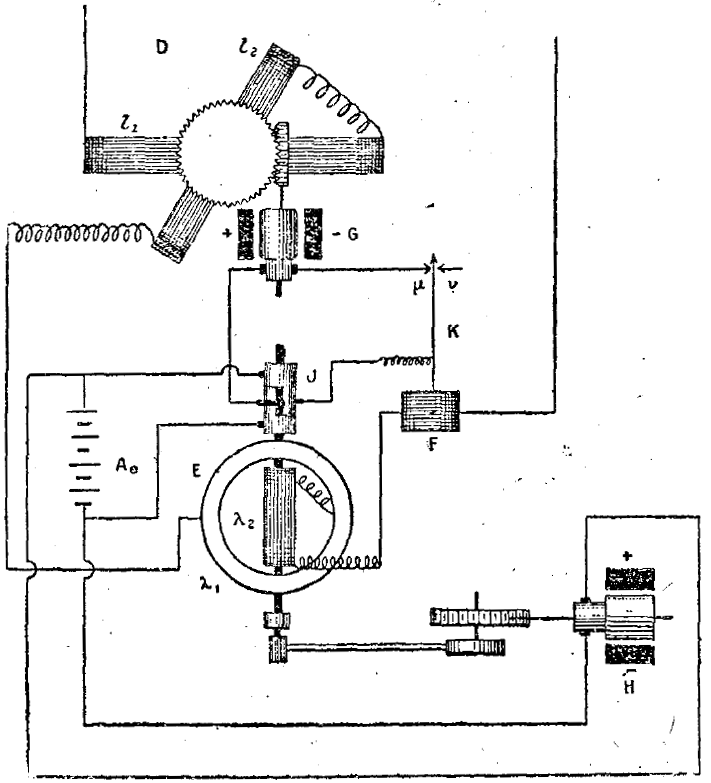
\includegraphics[width=0.9\textwidth]{img/extremum_seeking_controller.png}
\caption[Schematics of one of the first adaptive
controllers.]{Schematics of one of the first adaptive
controllers in the literature, implemented in
hardware.~\citenum{Leblanc:1922:Electrification}}
\label{fig:extremum-seeking-controller}
\end{marginfigure}

\lettrine{C}{ontrollers} that are able to adjust themselves to different
environmental conditions are usually subsumed under the umbrella term
``adaptive control''. Adaptivity is an important concept because there is
always a discrepancy between assumed models and the real world. In fact, for
many control systems a big proportion of development time is spent in
hand-crafting and tuning models. Adaptive control systems aim at learning
models at runtime, or at adjusting them if the environment is changing.

\margincite{Leblanc:1922:Electrification} The idea of adaptive control is quite
old, and many sources (\eg\cite{Ariyur.Krstic:2003:Real}) report the paper by
\citetext{Leblanc:1922:Electrification} as the first paper on this topic, see
Figure~\ref{fig:extremum-seeking-controller} for an illustration of the hardware
implementation. Since then, adaptive controllers have found many applications in
the automatic control of technical systems.

Unfortunately, the term \emph{adaptive control} has no clear definition and the
meaning often depends on the author. For example, in their textbook on
this topic, \textcite{Astrom.Wittenmark:1994:Adaptive} define ``an adaptive
controller [as] a controller with adjustable parameters and a mechanism for
adjusting the parameters''. The definition of adaptive control now depends on
the definition of a parameter, which also is not always clear.

Usually, the states are expected to change more rapidly and as direct response
to control actions and disturbances. Parameters, on the other hand, are
changing more slowly and are therefore seen on a different time
scale.~\cite[\ts3.1]{Filatov.Unbehauen:2004:Adaptive}\iss For example, while
position, velocity and acceleration are usually states, the physical properties
like weight or length of mechanical components are parameters. But also
slowly-varying states like the angle of attack of a plane can be seen as
parameters, since they change slowly, but govern other parts of the overall
dynamics. In hierarchical control systems, the states of a higher level can be
viewed as parameters of a lower one.

\section{Types of Adaptive Controllers}

Typically, adaptive controllers are classified into four different types of
adaptive control schemes
\margincite{Astrom.Wittenmark:1994:Adaptive}%
\margincite{Sastry.Bodson:2011:Adaptive}%
\citenum{Astrom.Wittenmark:1994:Adaptive, Sastry.Bodson:2011:Adaptive}:
\begin{description}
  \item[Gain Scheduling]
  This is the simplest case of an adaptive control system. Based on a
  pre-defined condition (for example, one of the states or parameters being in a
  certain  range), the control system switches between different setpoints or
  operating  conditions. A static feedback control law is provided for every
  setpoint. The  system is adaptive because the local controllers are tuned for
  each setpoint
  individually.~\cite{Leith.Leithead:2000:Survey}
  \item[Model-Reference Adaptive Control] This is a form of extremum seeking
  control, where a performance criterion based on a reference trajectory is
  optimized by parameter tuning. Usually this is done with a gradient-based
  optimization scheme, where the gradients are evaluated by numeric
  differentiation.~\cite{Landau:1974:Survey}
  \item[Self-Tuning Regulators] This is a model-based control strategy. A model
  of the system dynamics is learned or maintained online (\eg via parameter
  tracking in a parametric model). The model of the system is then used to
  calculate a controller with standard model-based control
  techniques.~\cite{Astrom.Wittenmark:1973:Self}
  \item[Dual Control\footnotemark] \footnotetext[1][3mm]{Dual control is
  an integral part of this thesis and will be covered in depth in
  Part~\ref{par:dual-control}.}This is the theoretically ideal way of performing
  adaptive control. An optimal dual controller would perform nonlinear
  stochastic optimal control on a system state that comprises both the states
  and the belief over the system dynamics. This type of controller is of such
  complexity that it is challenging to apply it in
  practice.~\cite{Wittenmark:1995:Adaptive}
\end{description}

Figure~\ref{fig:methods-classification} shows an overview of adaptive control
methods in relation to time of information acquisition.  While all adaptive
control methods are online methods, only dual control takes future measurements
into account.

\begin{figure}%
  \centering
  \inputTikZ{methods_classification}%
  \caption[Classification of adaptive control methods.]{Classification
of adaptive control methods, based on the time of information acquisition
(left to right) and the use of a model (top and bottom).}
  \label{fig:methods-classification}
\end{figure}

Note the distinction between model-free and model-based adaptive controllers.
From the above classifications, \emph{gain scheduling} and
\emph{model-reference adaptive control} are model-free, which means that they
are tuning a control-law\footnote{A control-law is sometimes also called
``policy'', especially in the reinforcement learning community.} directly. The
other two classes, \emph{self-tuning regulators} and \emph{dual control},
qualify as model-based schemes. This means that the model of the process is
adapted and a controller is synthesized from this model according to some
principle.

\section{Model Identification Adaptive Control}

The definition of adaptive control by \textcite{Astrom.Wittenmark:1994:Adaptive}
is relatively broad and can sometimes lead to confusion. Also, the distinction
between adaptive and non-adaptive is much harder to make for model-free
controllers than for model-based ones.\footnote{Essentially all model-free
controllers (except static state-feedback controllers) are adaptive because
they depend on changing parameters. This complicates the discussion quite a
bit.}
In the following, we therefore only consider model-based controllers, where we
assume that the system is governed by a true, but unknown, dynamics function
\begin{equation}
  x_{\tk+1} = f_\tk(x_\tk,u_\tk)
\end{equation}
that depends on the states $x$, the inputs $u$ and the time instance $\tk$. The
adaptive controller builds or updates an estimate $\hat f_\tk$ of the true
dynamics $f_\tk$ and uses it to calculate the control input
\begin{equation}
  u_\tk = c(\hat f_\tk, x_\tk),
\end{equation}
where $c$ is the model-based controller.\footnote{In the case of optimal
control, also a cost function $l_\tk$ would be necessary.}
Consequently, the controllers in this thesis can all be seen as model
identification adaptive controllers in the broader context of adaptive control.

\begin{figure}
  \center%
  \inputTikZ{MIAC_structure}%
  \caption[Structure of a model identification adaptive controller.]{
  Structure of a model identification adaptive controller.
  The estimator maintains a model $\hat f$ of the dynamics which is used by the
  controller together with the state $x$ to generate the control signal $u$.}
\end{figure}

\begin{definition}
  A model identification adaptive controller generates control inputs using
  an continually estimated model of the uncertain and possibly time-varying
  system dynamics.
\end{definition}

Henceforth, we use \emph{adaptive control} as a synonym for \emph{model
identification adaptive control} to simplify reading.

\pagebreak[4]

\section{System Identification and Adaptive Control}

Sometimes there is confusion between system identification
\cite{Ljung:1999:System} (in combination with a regular controller) and adaptive
control. This comes from the fact that both techniques use similar mathematical
methods. The difference lies in the time of information acquisition: While
system identification is done offline and provides a model for a controller,
adaptive control is an online method. While some types of adaptive control even
try to predict the process of information acquisition to the future, all
adaptive methods use the measurements during runtime to adjust the controller
(see also Figure~\ref{fig:methods-classification}).

It is clear that both system identification as well as adaptive control can
``adapt'' to different systems, but while an adaptive controller does the
learning online while controlling, system identification is separate from the
controller. Once the system identification is done, a controller is synthesized
and subsequently used in the control problem. Usually parameters that do not
change between the identification and the use of the control system are
identified with system identification. Other parameters can only be identified
online, either because they are subject to change or because the specific
problem instance can not be identified in advance.

\section{Adaptivity and Robustness}

Adaptivity is not the only way to deal with uncertainties in the model or the
environment. Another possible option is robust control
\cite{Zhou.Doyle:1998:Essentials}. In robust control systems, the controller is
designed to be resilient against uncertainties. This means that deviations in
the nominal parameters and disturbances do not endanger the system's stability.
This is usually done by considering worst case examples and controlling the
system in a way that all worst case examples are still stable.

If a control system is robust to parameter changes, one could argue that
adaptivity is not necessary. But there are still reasons to design adaptive
systems as well. Because robust control systems need to be compatible with
multiple worst case instances of a given problem, in many situations
infeasibility can arise: Not for all scenario distributions or combinations of
worst cases a robust controller does
exist.~\cite{Calafiore.Campi:2006:Scenario}\iss But also when feasibility is
given for the uncertain system, robust control trades performance for worst case
stability. If the control system is adaptive, the performance level can be much
higher after the system is learned because many of the unlikely examples can be
ruled out by the learning process.

Of course, adaptivity and robustness are not exclusive. A robust control system
can be designed relative to the current state of an adaptive control system,
combining the features of both.~\cite{Ioannou.Sun:1996:Robust}


\cleardoublepage
\phantomsection
\part{Nonparametric Disturbance Correction}
\label{par:predictive-disturbance-control}

\chapter{Gaussian Processes for Periodic Error Correction}
\label{ch:periodic-error-correction}

\lettrine{S}{crews and gears} are not the only source of periodically
recurring errors in dynamical systems. Every system that is tied to the
ubiquitous day-night cycle (like building control or energy systems) or to
recurring movements (like a beating heart or a satellite) suffers from
periodic errors. Since these effects are often small relative to the
required control precision, they are in practice usually neglected in the
controller design. For high-precision control systems, however, such errors can
be the dominant source of problems.

Correcting errors only after they are measured leads to a delay in the error
correction. If the errors can be anticipated, the control performance can be
significantly improved. While stochastically arising errors can not be
preempted systematically, periodic effects are amenable for prediction: Since
their future resembles their past, extrapolation is easier and more structured.
Based on this idea, we present a framework for identification and control of
periodic effects. Our framework continually performs identification at runtime,
\margincite{Kalman:1960:New}%
\margincite{Erm.Sandrock:2003:Adaptive}%
\margincite{Crassidis.Markley:1997:Predictive}%
\margincite{Sarkka:2013:Bayesian}%
\margincite{Yuen.Novotny.ea:2008:Quasiperiodic}%
\margincite{Kocijan.Murray-Smith.ea:2004:Gaussian}%
\margincite{Aswani.Gonzalez.ea:2013:Provably}%
\margincite{Tanaskovic.Fagiano.ea:2013:Adaptive}%
\margincite{Hennig:2011:Optimal}%
\margincite{Ko.Fox:2009:GP-BayesFilters}%
and is thus applicable to stochastic time varying systems.

The correction of periodic errors has repeatedly been studied. The ``Very Large
Telescope'' uses an internal parametric model for the known error sources, and
a Kalman filter \citenum{Kalman:1960:New}
as an estimator for the model
parameters.~\citenum{Erm.Sandrock:2003:Adaptive} High-precision tracking of
spacecrafts on periodic trajectories was addressed by
\citeauthor{Crassidis.Markley:1997:Predictive}
\citenum{Crassidis.Markley:1997:Predictive}, based on predictive filtering using
an extended Kalman filter. To predict the beating motion of a human heart,
extended Kalman filtering for state estimation was used by
\citeauthor{Yuen.Novotny.ea:2008:Quasiperiodic}
\citenum{Yuen.Novotny.ea:2008:Quasiperiodic}, allowing the nonlinear model to
change over time. Concerning the use of learning based models for control, there
is a wide range of literature available in the context of adaptive control. For
methods based on model predictive control see, \eg the recent works
\citenum{Kocijan.Murray-Smith.ea:2004:Gaussian},
\citenum{Aswani.Gonzalez.ea:2013:Provably},
\citenum{Tanaskovic.Fagiano.ea:2013:Adaptive}.

In contrast to previous methods for periodic error correction, the approach
presented here does not rely on a pre-specified finite-di\-men\-sion\-al model
class. Instead, we propose a nonparametric framework based on Gaussian process
(GP) regression that is frequently used for system identification. It is closely
related to least-squares regression, which is the most commonly employed
technique in system identification, but is based on a probabilistic
interpretation, which can be used to guide exploration during identification
\citenum{Hennig:2011:Optimal}. There is recent work on using GPs for state
filtering \citenum{Ko.Fox:2009:GP-BayesFilters} and on modeling and control of
nonlinear systems \cite{Pillonetto.Dinuzzo.ea:2014:Kernel},
\cite{Hall.Rasmussen.ea:2012:Modelling}. The idea of using the learned model in
predictive control is conceptually similar to
\cite{Kocijan.Murray-Smith.ea:2004:Gaussian},
\cite{Aswani.Gonzalez.ea:2013:Provably}, \cite{Maciejowski.Yang:2013:Fault},
with the key difference that we use a GP to predict time varying effects.

A Gaussian process model is parametrized
by two objects: mean and covariance function.  When used in system
identification, in particular the choice of covariance function has a strong
effect on performance, and requires consideration of the dynamics to
be identified. Although the literature knows ``universal'' covariance functions
that can technically approximate any continuous function
\margincite{Steinwart:2002:On}\margincite{Micchelli.Xu.ea:2006:Universal}%
\citenum{Steinwart:2002:On,Micchelli.Xu.ea:2006:Universal}, this notion only
applies in the infinite limit, and can be subject to extremely slow convergence
\margincite{van-der-Vaart.van-Zanten:2008:Rates}%
\margincite{van-der-Vaart.van-Zanten:2011:Information}%
\citenum{van-der-Vaart.van-Zanten:2008:Rates,
van-der-Vaart.van-Zanten:2011:Information}. Hence, the choice of covariance
function is often critical in practice.

In this chapter, the focus lies on the identification of quasiperiodic systems
(Section~\ref{sec:problem_statement}) by using a specific model class involving
periodicity (Section~\ref{sec:quasiperiodic_covariance_function}). The
identification of hyperparameters is performed by exploiting the structure of
the problem at hand (Section~\ref{sec:custom-optimisation}). We focus on the
case where the only nonlinearity is the periodic effect, and use model
predictive control to achieve optimal closed-loop performance
(Section~\ref{sec:standard_mpc}). A reformulation in the form of a tracking
problem is proposed, which offers simple implementation and facilitates
analysis of the control performance (Section~\ref{sec:tracking_mpc}). To show
the qualitative properties of this framework, we apply it to a simulated,
educational problem (Section~\ref{sec:gp-pec-experiments}). While GPs and MPC
are well studied techniques, the main contribution of this work is a
combination that is tailored to quasiperiodic functions, allowing for
extrapolation and efficient computation, which is crucial for online
identification and control.

\section{Problem Statement}
\label{sec:problem_statement}

Consider the continuous dynamical system
\begin{align}
\label{eq:problem}
  \dot x(t) &= A_c x(t) + B_c u(t) + g(t),
\end{align}
composed of a linear system with continuous dynamics matrices $A_c$ and $B_c$,
and a nonlinear time varying function $g:\Re_+ \to \Re^\ns$, where $x\in\Re^\ns$
denotes the state and $u\in\Re^\ni$ the input. For simplicity, full state
measurement is assumed. The structure of \eqref{eq:problem} could be chosen more
generally---Gaussian process models can also learn nonlinear functions of the
state and input. We opt for this linear formulation with nonlinear external
reference here to keep the resulting control problem conceptually clear and
\margincite{Allgower.Badgwell.ea:1999:Nonlinear}%
computationally simple. If needed, the definition can also be adapted to a
nonlinear system using a nonlinear model predictive control technique
\citenum{Allgower.Badgwell.ea:1999:Nonlinear}.

The disturbance function $g(t)$ captures nonlinear time dependent effects, in
particular we focus on systems exhibiting some form of periodic behavior.
Systems with time dependent errors of periodic characteristic appear in
different application areas, such as building temperature control
\cite{Gondhalekar.Oldewurtel.ea:2010:Least-restrictive}, beating-heart surgery
\cite{Yuen.Novotny.ea:2008:Quasiperiodic} or electrical power grids
\cite{Taylor.McSharry:2007:Short}.
For strictly periodic functions, there exists a constant period $\lambda$, such
that $g(t+n\lambda)=g(t)$ for $n\in\Nat$. However, error sources in real systems
are often not perfectly periodic in this sense, they show various forms of
phase-shift, deformation and desynchronization. To address this issue, we
generalize to consider locally periodic functions. These are functions for which
$g(t) \approx g(t+n\lambda)$ for $n\lambda \ll \ell$ and $g(t) \not\approx
g(t+n\lambda)$ for $n\lambda\gg\ell$, where $\ell$ is some measure of temporal
locality. Intuitively speaking, local periodicity means that the periodicity is
not strict, \ie variations are allowed. In particular, this covers functions
that vary on a slower time-scale, \eg a decaying oscillation or an oscillation
with long-term change in shape.

We consider the case where a linear model (matrices $A_c$ and $B_c$) is
available and the goal is to infer the disturbance function $g(t)$ online from
measurements. This is motivated by the fact that often a nominal model is
derived either from physical considerations or an offline system identification
step.

At every measurement time $t_k$, the system goes
through the following process:
\begin{enumerate}
  \item Measure $x(t_k), \dot x(t_k)$
  \item Construct observation for $g(t_k)$, update model for $g(t)$
  \item Compute control input $u(x(t_k),g(t_k))$ and apply to the system
\end{enumerate}

\section{GPs for Quasiperiodic Functions}
\label{sec:gps_for_quasiperiodic_functions}

GP regression is a general framework for nonlinear regression, see
Chapter~\ref{ch:gaussian-processes} for an introduction. Note that in the
current chapter we use the time $t$ as the function argument, since this
chapter is concerned with time-series forecasting.

As mentioned above, in the context of our particular setup, the GP framework
may in fact also be used to construct probabilistic models for fully nonlinear
systems $g(x,u,t)$, without major changes. However, we focus on
the simpler case of $g(t)$, allowing for direct incorporation in stochastic
predictive control techniques.

This section proposes a covariance function suitable for the identification
of quasiperiodic functions and presents an efficient technique for
hyperparameter optimization.

\subsection{Quasiperiodic Covariance Functions}
\label{sec:quasiperiodic_covariance_function}

The way to construct a periodic hypothesis class, and the central idea of this
chapter, is to construct a covariance function that focuses prior probability
mass on locally periodic functions. Among the most popular kernels for
regression purposes is the square exponential\footnote{The square exponential
kernel is also known as \emph{squared exponential kernel}, \emph{Gaussian
kernel}, or \emph{radial basis function}.} kernel
\vspace{-\baselineskip}
\begin{equation}
\label{eq:square-exp}
k_{\mathsc{se}}(t,t';\ell_\mathsc{se}) =
\exp\left(-\frac{|t-t'|^2}{2\ell_\mathsc{se}^{2}}\right),
\end{equation}
with length-scale $\ell_\mathsc{se}$. This kernel gives a stationary model
which does not allow for structured extrapolation.
\citeauthor{MacKay:1998:Introduction} proposed a periodic covariance function,
based on a sine-transformation of the input \cite{MacKay:1998:Introduction}
\begin{equation}
\label{eq:periodic}
k_\mathsc{p}(t,t';\ell_\mathsc{p},\lambda) =
\exp\left(-\frac{2\sin^2\left(\frac{\pi}{\lambda}
(t-t')\right)}{\ell_\mathsc{p}^2}\right),
\end{equation}
with length-scale $\ell_\mathsc{p}$ and period-length $\lambda$.
Function values $g(t), g(t')$ jointly sampled from Gaussian process
priors with this covariance function are perfectly correlated  if $|t-t'| =
\lambda$, resulting in identical function values for points that are one period
length apart. Thus, sampled functions are perfectly periodic with period
$\lambda$. Within this period length, samples vary on a typical regularity
length scale of $\delta = \sin^{-1}(\ell_\mathsc{p} /2)\lambda/\pi$, over a
range with standard deviation $\theta=1$ (Figure~\ref{fig:covariance}).

\begin{figure}
\setlength\figurewidth{0.9\textwidth}%
\setlength\figureheight{0.309\figurewidth}%
\centering%
\footnotesize%
\subfloat[Covariance functions]{\inputTikZ{covariance_functions}
\label{fig:covariance_functions}}\\
\subfloat[Samples from GPs with these covariance
functions]{\inputTikZ{covariance_samples} \label{fig:covariance_samples}}
\caption[Kernel combination, covariance function and samples.]{Kernel
combination, covariance function and samples. {\bfseries Top:} The compound
kernel $k_\mathsc{c}$ (\ref*{p:pec-cov-comb},\eqref{eq:comp-kernel}) is the
product of $k_\mathsc{se}$ (\ref*{p:pec-cov-se}, \eqref{eq:square-exp}) and
$k_\mathsc{p}$ (\ref*{p:pec-cov-per}, \eqref{eq:periodic}). {\bfseries Bottom:}
Samples drawn from Gaussian process priors using these covariance functions
(same colors). Samples using the periodic kernel are perfectly periodic, while
samples using the compound kernel are only periodically similar on a scale
controlled by the parameter $\ell_\mathsc{se}$ of (\ref{eq:comp-kernel}). This
local periodicity can be used to increase modeling flexibility.}
\label{fig:covariance}
\end{figure}

For many systems, strict periodicity is too strong an assumption. For example,
the weather is periodic, but also stochastic, which has an effect on the
periodic temperature in a building. Therefore, modeling external errors with
perfect periodicity can lead to severe overfitting and low extrapolation
performance. To weaken the perfect correlation, we use the fact that the kernel
property is closed under multiplication and addition (\ie kernels form a
semi\-ring \cite[\ts4.2.4]{Rasmussen.Williams:2006:Gaussian}): Although the
product of two Gaussian processes is not a Gaussian process, the product of two
kernel functions is also a kernel and therefore a valid covariance function for
a Gaussian process.

This property of covariance functions is useful to construct composite
covariance functions, either automatically from data
\cite{Duvenaud.Lloyd.ea:2013:Structure} or manually. Since we assume access to
physical knowledge about the system, we constructed a suitable kernel in a
qualitative manner. Multiplying the periodic kernel with a broad
square exponential gives another kernel whose corresponding Gaussian process
condenses mass at periodic functions that change over time
\begin{equation}
\label{eq:comp-kernel}
k_\mathsc{c}(t,t';\theta^2,\ell_\mathsc{se},\ell_\mathsc{p},\lambda) = \theta^2
\cdot
k_{\mathsc{se}}(t,t';\ell_\mathsc{se})
\cdot k_\mathsc{p}(t,t';\ell_\mathsc{p},\lambda),
\end{equation}
with signal variance $\theta^2$ and the other parameters as stated above. This
kernel considers two input times similar if they are similar under both the
square exponential \emph{and} the periodic kernel. If $\ell_\mathsc{se} \gg
\lambda$, this allows encoding a decay in the covariance over several
oscillations. The different covariance functions are shown in
Figure~\ref{fig:covariance} (a), exemplary randomly sampled functions from
Gaussian processes with those covariance functions are shown in
Figure~\ref{fig:covariance} (b). The posteriors of GPs with aperiodic and
periodic covariance, trained on periodic data, are shown in
Figure~\ref{fig:kernels}. In the region far away from data points the
predictions are equal, whereas close predictions show significantly more
structure with the locally periodic kernel.

\begin{figure}
\centering%
\footnotesize%
\subfloat[SE kernel]{\inputTikZ{bad_kernel}}\\
\subfloat[Locally periodic kernel]{\inputTikZ{good_kernel}}
\caption[Comparison of Gaussian process posteriors for structured
extrapolation.]{Comparison of Gaussian process posteriors (posterior mean
function as thick line, shaded region covers two marginal standard deviations)
arising from the same periodic data (\refpoints{p:bad-kernel-data}) for the
square exponential kernel (\ref*{p:bad-kernel-mean}/\ref*{p:bad-kernel-sd}) and
a product of periodic and square exponential kernel
(\ref*{p:good-kernel-mean}/\ref*{p:good-kernel-sd}). The locally periodic kernel
provides a richer extrapolation, which can be used for improved predictive
control.}
\label{fig:kernels}
\end{figure}

Figure~\ref{fig:kernels} (b) illustrates the key benefit of this approach: With
increasing distance from data, the prediction degrades gracefully back to the
zero mean. If a not perfectly periodic function would be predicted with a
purely periodic kernel, prediction and reality could run out of phase over
time, leading to bad predictive behavior. The proposed locally periodic
covariance function circumvents this problem.

\subsection{Custom Parameter Optimization}
\label{sec:custom-optimisation}

The combined kernel (\ref{eq:comp-kernel}) has four hyperparameters,
which will henceforth be subsumed in the vector $\boldsymbol{\eta}
\ce
(\theta^2,\ell_\mathsc{se},\ell_\mathsc{p},\lambda)$. This includes the
period length $\lambda$ of the periodicity. Inferring good values for
$\boldsymbol{\eta}$ is
important for good modeling performance. The parameter optimization is done
by type-II maximum likelihood / maximum a-posteriori, as described in
Section~\ref{sec:parameter-fitting}. However, using this optimization scheme in
a non-modified (``vanilla'') fashion usually does not work in periodic or
quasiperiodic settings.

The log-likelihood surface for $\boldsymbol{\eta}$ is, especially
for periodic likelihoods,
not convex. Figure~\ref{fig:maximum_likelihood} shows a slice through this
surface along the periodicity parameter $\lambda$ for a quasiperiodic dataset.
Standard numerical optimizers will, thus, usually return suboptimal local
extrema of this function. An interesting observation in our specific context is
that the periodic structure of the covariance function and the data is reflected
in this hyperparameter likelihood as well. The reason for this is a harmonic
effect: If the data has a true period of $\lambda$, then periodic functions
whose periodicity is an integer multiple of $\lambda$ also fit the data well,
resulting in low values in the log likelihood
\begin{equation}
\label{eq:gp-pec-log-likelihood}
  \log p(\mathbf{y} | \mathbf{t},\boldsymbol{\eta}) = - \frac{1}{2} \mathbf{y}\T
K(\boldsymbol{\eta})\inv
  \mathbf{y} - \frac{1}{2} \log \left|K(\boldsymbol{\eta})\right| -\frac{N}{2}
\log 2\pi.
\end{equation}

Intuitively, this can be compared to a function with periodicity $\lambda$,
which could also be considered as a function with period length $2\lambda$. To
see this, recall from Figure~\ref{fig:covariance} that the periodic
functions can have an arbitrary recurring pattern in each repetition. By
inspecting Equation~\eqref{eq:gp-pec-log-likelihood}, we can gain intuition and
notice that the likelihood is a nonlinear function of terms of the form
\eqref{eq:periodic}. Since each of these terms is periodic in $\lambda^{-1}$,
the overall function will show periodicity in that term.

This harmonic structure can be exploited by means of a heuristic to increase
numerical stability of the optimizer. We designed a customization of a
numerical optimizer, outlined in Algorithm~\ref{alg:custom-optimisation}, that,
after convergence to a local minimum
$\boldsymbol{\eta}=(\theta^2,\ell_\mathsc{se},\ell_\mathsc{p},\lambda)$, also
evaluates the
function value at
$\boldsymbol{\eta}'=(\theta^2,\ell_\mathsc{se},\ell_\mathsc{p},\frac{\lambda}{2}
)$. If the
negative log likelihood at this location is lower, the optimal value and its
location is updated, and the bisection is repeated. The locations that are
iteratively proposed during the loop (Line 4 of
Algorithm~\ref{alg:custom-optimisation}) are shown as
vertical lines (\ref*{p:log-search}) in Figure~\ref{fig:maximum_likelihood}.
This approach uses the otherwise problematic harmonic structure in the
hyperparameter optimization to find better optima.

\begin{figure}%
\centering%
\footnotesize%
\inputTikZ{log_posterior}%
\caption[Slice through the likelihood surface.]{Slice through the
likelihood surface along the dimension of the hyperparameter $\lambda$, defining
the period length of $g$. Shown are the logarithm of the type-II marginal
likelihood (\ref*{p:log-likelihood}) and the logarithm of the posterior
distribution (\ref*{p:log-posterior}). The shape of the log posterior is
dominated by the likelihood, indicating that most prior assumptions are
dominated by the observed data. The meaning of the vertical lines is explained
in Section~\ref{sec:custom-optimisation}.}
  \label{fig:maximum_likelihood}
\end{figure}

\vspace{1.1cm}
\begin{algorithm}
\vspace{-1.1cm}
\hrule
\vspace{2mm}
\begin{algorithmic}[1]%
\State $\boldsymbol{\eta} \ce
(\theta^2,\ell_\mathsc{se},\ell_\mathsc{p},\lambda)$
\Comment{initial guess}
  \State $\boldsymbol{\eta} \gets$
\Call{Locally\_Optimize}{$\boldsymbol{\eta}$} \Comment{use std.
optimizer}
    \Loop
      \State $\boldsymbol{\eta}' \gets
(\theta^2,\ell_\mathsc{se},\ell_\mathsc{p},\frac{1}{2}\lambda)$ \Comment{make
proposal}

      \If{$\text{nll}(\boldsymbol{\eta}') > \text{nll}(\boldsymbol{\eta})$}
\Comment{compare neg. log
lik.}
        \State \textbf{break} \Comment{reject and leave loop}
      \Else
        \State $\boldsymbol{\eta} \gets \boldsymbol{\eta}'$
\Comment{accept proposal}
      \EndIf
    \EndLoop
    \State \textbf{return} $\boldsymbol{\eta}$
% \EndProcedure
\end{algorithmic}%
\caption[Customized parameter optimization.]{Customized parameter
optimization. After the convergence of the standard optimizer, the
likelihoods for halved period lengths are evaluated. The period length with the
lowest negative log likelihood is accepted.}%
\label{alg:custom-optimisation}%
\vspace{1mm}
\hrule
\end{algorithm}

\subsection{Sampling Methods for Parameter Identification}

Instead of using only a maximum likelihood or maximum a-posteriori point
estimate, theoretically the goal would be to compute the marginal
\vspace{-\baselineskip}
\begin{equation}
  p(g) = \int p(g|\boldsymbol{\eta}) p(\boldsymbol{\eta}) d\boldsymbol{\eta}
\end{equation}
using a prior density $p(\boldsymbol{\eta})$
\cite[\ts5.2]{Rasmussen.Williams:2006:Gaussian},
which can only be performed approximately at high computational expense. One
comparably elaborate and precise way to approximate the posterior distribution
over $\boldsymbol{\eta}$ and to marginalize over the unknown
parameters $\boldsymbol{\eta}$ is sampling,
using a Markov chain Monte Carlo (MCMC) method. We found \emph{shrinking-rank
slice sampling} \cite{Thompson.Neal:2010:Slice} to be particularly well-suited
for this task and implemented the method for a comparison between the MAP
point-estimate and MCMC sampling.

The left column of Figure~\ref{fig:ml_vs_sampling} shows the resulting marginals
on the function $g$ at two different points in the learning process for a
quasiperiodic system. As expected, the posterior uncertainty is high after
only a few observations, in particular after less than one full period, but
collapses to a highly confident distribution after several periods of
observations have been collected.

The right column of Figure~\ref{fig:ml_vs_sampling} shows the Gaussian process
point estimates for $g$ resulting from MAP inference. From the figure, it is
clear that point estimation leads to a more limited, and generally overly
confident extrapolation model, especially in early phases of learning, when the
dataset does not yet cover several periods. However, MAP offers two advantages
that make it attractive from an applied perspective: The first one is
computational cost---MCMC sampling can be orders of magnitude more expensive
than optimization for a MAP estimate. The second one is an algebraic one: MCMC
estimates are mixtures of Gaussian process models (see
Figure~\ref{fig:ml_vs_sampling}). This means the overall model for the
regression function defined by these models is an object challenging to work
with. Therefore, applications often use the computationally much less taxing MAP
inference.

\begin{figure*}
\setlength{\figurewidth}{0.45\columnwidth}%
\setlength{\figureheight}{0.25\columnwidth}%
\centering%
\footnotesize%
\subfloat{\inputTikZ{ml_vs_sampling_2}\hspace{5mm}}%
\subfloat{\inputTikZ{ml_vs_sampling_1}\hspace{5mm}}\\%
\subfloat{\inputTikZ{ml_vs_sampling_4}\hspace{5mm}}%
\subfloat{\inputTikZ{ml_vs_sampling_3}\hspace{5mm}}%
\caption[Comparison of MCMC inference to MAP inference.]{Comparison of Markov
chain Monte Carlo inference (left column) with the maximum a-posteriori point
estimate (right column) on hyperparameters of the Gaussian process model.
{\bfseries Top:} Initial phase of learning, after only a few observations.
{\bfseries Bottom:} Convergence after observation of several periods.}
\label{fig:ml_vs_sampling}
\end{figure*}

\section{GP Predictions in Model Predictive Control}
\label{sec:control}
Popular control frameworks supporting the incorporation of feed-forward model
predictions include linear quadratic regulator (LQR)
\clearpage \noindent
techniques \cite[\ts8.3]{Ogata:1995:Discrete}, or model predictive control (MPC)
\cite{Rawlings.Mayne:2009:Model}. See
Chapter~\ref{ch:discrete-time-optimal-control} for an introduction to these
methods.

For periodic error correction, we employ an online MPC framework, computing
the optimal control input by solving an optimization problem for each measured
state. This allows for direct incorporation and updating of the GP model
as well as system constraints, such as input constraints.

\subsection{Discrete-time MPC formulation}
\label{sec:standard_mpc}

A discrete-time MPC approach is used based on the discretization of the model
\eqref{eq:problem}
\begin{equation}
  \label{eq:pec-discrete-system}
  x_{k+1} = A x_k + B u_k + a_k,
\end{equation}
where $A$ and $B$ are obtained from a zero-order-hold discretization and
$a_k$ is a discretization of choice of $g(t)$ at time $t_k$.

Since the optimal control input is computed at each sampling time based on the
current measured state, the model can be updated online. An important aspect
and advantage of combining online learning of a continuous time function with
MPC is the possibility to decouple the discretization from the sampling time.
While in a standard MPC setup, unmodeled effects only become apparent through
state measurements and therefore require fast sampling rates, the GP model
captures these effects and provides a continuous prediction of their evolution
in the future. As a result, the sampling time can be chosen as a multiple of
the discretization or prediction interval without sacrificing performance by
using the sequence of control inputs in between state measurements. It is clear
that an upper bound on the sampling time is imposed by the prediction horizon.

Since the prediction from the Gaussian process model is stochastic and provides
a distribution over future function values rather than one particular sequence,
stochastic MPC methods offer a natural framework to incorporate the GP model
and make use of the posterior model uncertainty. For an overview of recent
stochastic MPC methods, see \eg \cite{Kouvaritakis.Cannon:2014:Stochastic},
\cite{Mayne:2014:Model} and the references therein. The model uncertainty is an
important advantage over other nonparametric methods like kernel ridge
regression or regularized least squares, which do not provide posterior
uncertainty.

A common cost function in stochastic MPC for regulating the system state to the
origin is the expected value of the sum of stage costs
\vspace{-\baselineskip}
\begin{equation}
J(x_0,p(g),\mathbf{u}) \ce \mathbb{E}\left[\sum_{i=0}^{\HL}
l(x_i(p(g)), u_i) \right]
\end{equation}
where $p(g) = \GP(g;m^{|\mathbf{t},\mathbf{y}},k^{|\mathbf{t}})$ denotes the
posterior distribution over the function $g$. If the stage cost $l$ is chosen to
be quadratic (which is the case for many practical MPC problems) and since the
inputs are deterministic and the GP posterior is Gaussian, the expected value is
equivalent to using the mean of the state evolution, i.e.\ the mean GP
prediction of $g(t)$ in dynamics \eqref{eq:problem}. The most common stochastic
MPC problem hence results in a deterministic formulation by using the GP
posterior mean $\tilde g(t) = m^{|\mathbf{t},\mathbf{y}}(t)$, and reduces to the
certainty equivalent controller.

We consider the case of quadratic stage cost in the following. Since the true
function $g(t)$ is unknown, a discrete-time system describing the mean of the
state trajectory is approximated by replacing $a_k$ in
\eqref{eq:pec-discrete-system} with $\tilde a_k$, obtained by discretizing the
mean of the GP prediction $\tilde g(t)$. $\tilde{\cdot}$
denotes the estimate of the true function inferred from data, and emphasizes
that these are generally not the same. The resulting discrete-time system can
directly be used in a standard MPC formulation.

\subsection{Tracking MPC}
\label{sec:tracking_mpc}

We propose a different formulation in the following, which simplifies
implementation by transforming the regulation problem into a linear tracking
problem. The state of the mean discrete-time system at prediction time step
$k+n$, starting from state $x_k$ at time step $k$ is given by:
\begin{equation}
\label{eq:state-evolution}
  \tilde x_{k+n} = A^n x_k + \sum_{m=1}^{n} A^{m-1} B u_{k+n-m} +
\sum_{m=1}^{n} A^{m-1} \tilde a_{k+n-m},
\end{equation}
where $\tilde a_k$ is the discretization of the GP prediction
$\tilde g$. This is the sum of the linear system and a system driven by
$\tilde a_k$. The MPC problem for regulating system
\eqref{eq:pec-discrete-system} to the origin can be reformulated as a tracking
problem for the linear system, tracking a nonlinear reference.

The reference signal is generated from the GP prediction according to
\eqref{eq:state-evolution}:
\begin{equation}
\label{eq:reference-generation}
  \mathbf{x}^\text{ref} = \left[\tilde a_{k+1}\quad
\cdots\quad \sum_{m=1}^{n} A^{m-1} \tilde a_{k+n-m}\right].
\end{equation}
The resulting MPC problem is given by
\begin{subequations}
\begin{align}
  (\mathbf{x}^*, \mathbf{u}^*)=\underset{\mathbf{x,u}}{\argmin} \quad
&\sum_{n=0}^{\HL} l(x_n - x^\text{ref}_n, u_n)  \\
\text{s.t.}\quad
& x_{n=0} = x(t_k) \\
& x_{n+1} = A x_n + B u_n \\
& u \in \mathbb{U}
\end{align}
\end{subequations}
where $\mathbb{U} \subseteq \mathbb{R}^\ni$ is a polytopic set defining the
input constraints, $\mathbf{x}\ce[x_0,\dots,x_\HL]$ is the state trajectory and
similarly for $\mathbf{u}$. The resulting problem is a quadratic program that
can be solved efficiently using available optimization software (\eg
\cite{Grant.Boyd:2014:CVX}) or fast MPC techniques proposed in recent years,
such as code generation (\eg \cite{Domahidi:2012:FORCES}). Because this is an
instance of a basic MPC technique, the standard properties of MPC apply. It also
allows for a more principled analysis of the closed-loop properties: Extensions
in the field of tracking MPC can be applied to ensure stability, such as
reference governors, or the periodic MPC approach in
\cite{Limon.Alamo.ea:2012:MPC}. Applying the modified tracking formulation in
\citenum{Limon.Alamo.ea:2012:MPC}, convergence can be guaranteed if the model
$\tilde g(t)$ converges to a periodic function.

\begin{remark}
The discrete-time model \eqref{eq:pec-discrete-system} with the predicted
nonlinear term $\tilde a_k$ can in principle be used in any linear or linearized
state estimation or control method based on state prediction. One example is the
Kalman filter. The nonlinear prediction from the GP can be incorporated into the
state prediction without complicating the Kalman filter equations. The
measurement update of the Kalman filter remains unchanged. The GP predictions
increase the performance by providing a better state estimate. This leads to
smaller correction terms and smaller posterior variance.
\end{remark}

\begin{remark}
Because the point-wise posterior of a Gaussian process is a Gaussian
distribution, state constraints can be included in the form of soft constraints,
penalizing the amount of constraint violation, or chance constraints, ensuring
constraint satisfaction with a certain probability
\margincite{Schwarm.Nikolaou:1999:Chance-constrained}%
\margincite{Ono.Williams:2008:Iterative}%
\citenum{Schwarm.Nikolaou:1999:Chance-constrained, Ono.Williams:2008:Iterative}.
\end{remark}

\begin{remark}
The approach can also be applied to stage cost functions and constraints that
do not allow for a deterministic representation using the GP model, \eg a
value-at-risk formulation involving the variance of the cost by using
sample-based methods to approximate the stochastic MPC problem
\margincite{Campi.Garatti.ea:2009:scenario}%
\margincite{Schildbach.Fagiano.ea:2014:Scenario}%
\citenum{Campi.Garatti.ea:2009:scenario, Schildbach.Fagiano.ea:2014:Scenario}.
GPs fit well in this framework by being generative models from which sample
trajectories can be easily drawn.
\end{remark}

\begin{remark}
Depending on the discretization, a trade-off between the mean and variance
of a quadratic cost function can be formulated as a deterministic optimization
problem using the posterior GP prediction:
\begin{subequations}
\begin{align}
  \Exp\left[ \frac{1}{2} x_n\Trans \SC_n x_n\right] &= \mu_n\Trans \SC_n \mu_n +
  \tr(\SC_n\Sigma_n),\\
  \Var\left[ \frac{1}{2} x_n\Trans \SC_n x_n\right] &= \mu_n\Trans \SC_n
\Sigma_n \SC_n
  \mu_n + \frac{1}{2} \tr(\SC_n\Sigma_n \SC_n\Sigma_n).
\end{align}
\end{subequations}
This is the case whenever the distribution $\N(\mu_n,\Sigma_n)$ of $a_k$ can be
directly obtained from the distribution of $g(t)$, \eg in the case of Euler
discretization.
\end{remark}

\section{Numerical Results}
\label{sec:gp-pec-experiments}

The presented method was implemented for a simple problem and evaluated in
simulation to show how the state evolution is anticipated by the use of the GP
prediction. In Chapter~\ref{ch:predictive-error-correction-for-telescopes},
this method will also be evaluated on an experimental application in hardware.

\subsection{Implementation Details}
\label{sec:implementation_details}

Since in practice the state and derivative can not be measured directly, they
have to be approximated from potentially noisy measurements. A Kalman filter
\cite{Kalman:1960:New} can be used to estimate the state, which increases the
performance, especially when the measurement noise is high.

Since the function to be inferred acts as additional input to the dynamics,
observations of the disturbance are constructed from observations of the
\emph{change} in state, $\Delta x = x_{k+1} - x_k $. We therefore assume
$g(t)$ to be piece-wise constant, here a zero-order-hold linearization is used,
chosen to be at $t+\frac{1}{2}\Delta t$
\begin{equation}
  a_k = G g(t+\frac{1}{2}\Delta t), \qquad G = \int_0^{\Delta
t}e^{A\tau}d\tau,
\end{equation}
where $\Delta t$ is the sampling time. Note that this is only used to generate
the data point, the resulting GP model is still a continuous function.
The value $g(t+\nicefrac{1}{2}\Delta t)$ is obtained as solution of the linear
system
\begin{equation}
  G g(t+\frac{1}{2}\Delta t) \approx \left(x_{k+1} - A x_k - B u_k\right),
\end{equation}
which is the data point used to train the GP.

In the experiments presented in the following, the discretization of the
mean prediction $\tilde g(t)$ is obtained from the exact
discretization
\begin{equation}
\label{eq:affine_convolution}
 \tilde a_k = \intl_{0}^{\Delta t} e^{A_c\tau} \tilde g({(k+1)\Delta
t}-\tau)d\tau ,
\end{equation}
evaluated with a standard ODE-solver \cite{Dormand.Prince:1980:family}.

\subsection{A Simple Example}
\label{sec:toy_problem}

As a simple problem for providing intuition, consider the following linear
double integrator system with an additive time-periodic component $g(t)$:
\begin{fullwidth}\vspace{-\baselineskip}
\begin{equation}
\label{eq:toy-dynamics}
  \dot x(t) = \begin{bmatrix}0 & 1 \\ 0 & 0 \end{bmatrix}
  x(t) + \begin{bmatrix}0 \\ 1 \end{bmatrix} u(t) + g(t),
\qq
 g(t) = \begin{bmatrix}\sin(t) \\ \cos(1.3 t) \end{bmatrix}.
\end{equation}
\end{fullwidth}
The goal is to control the first state of the system to the origin. We use the
quadratic cost
\begin{equation}
  l(x_n,u_n) = \frac{1}{2} x_{n}\Trans \SC x_{n} + \frac{1}{2} u_n\Trans
  \CC u_n
\end{equation}
with diagonal state weight $\SC = \diag(100, 0)$.
The weight on the control input is set to $\CC=1$, allowing for
aggressive control behavior. The horizon length of the MPC is set to $\HL = 15$.
State and input constraints are omitted for simplicity.

The system was simulated numerically with a sampling rate of 1\unit{Hz}.
Figure~\ref{fig:toy_example} shows control inputs and resulting state
trajectories for a model predictive controller without information about the
disturbance $g$, and a model predictive controller using the posterior mean
functions of two periodic Gaussian process regressors as a model for $g$. One
GP is trained for each dimension of the disturbance.

After an identification phase in the first 5\unit{s} of the experiment, the GP
based controller shows a drastic performance improvement. Omitting this
identification phase, the root-mean-square (RMS) error, measured with respect
to the origin, drops by 90\unit{\%}, from 0.94 for the linear model to 0.097
for the GP based controller. Speaking more qualitatively,
Figure~\ref{fig:toy_example} also shows less residual structure in the
controlled state $x_1$. It is visible that control signals are applied earlier
when the prediction is used.

While the GP based controller is effective at reducing the periodic structure
from the first controlled state, the regression model itself remains able to
predict the periodic error correctly into the future, even when trained
exclusively on controlled states. This is possible because the regression model
is obtained from the controlled dynamics, so it can account for the shift of
periodicity from the states to the control input. This feature of the framework
is crucial for identifying controlled systems.

\begin{figure}
\centering
\footnotesize
\inputTikZ{toy_example}
\caption[Closed-loop input and output trajectories with MPC
control.]{Closed-loop input and output trajectories with MPC control.
MPC using a linear model (\ref*{p:toy-x-plain}) is compared to the GP based MPC
controller (\ref*{p:toy-x-gp}).}
\label{fig:toy_example}
\end{figure}

\section{Conclusion}

High-precision control of dynamical systems requires precise models, even of
minor external error sources. Where analytic models are not available, they can
only be constructed numerically from measurements of the system. Periodic error
sources are an especially promising domain in this regard, as they can be
extrapolated well into the future. We have studied a nonparametric modeling
framework based on a carefully crafted Gaussian process prior exhibiting a
weak, localized form of periodicity. Because Gaussian regression returns models
in the form of stochastic differential equations, they can be combined directly
with existing control frameworks. Integration into a model predictive control
scheme was investigated, which can evaluate the prediction at a desired temporal
resolution.

\chapter{Periodic Error Correction for Telescope Tracking}
\label{ch:predictive-error-correction-for-telescopes}

\begin{marginfigure}[1.9\baselineskip]
\centering%
\footnotesize%
  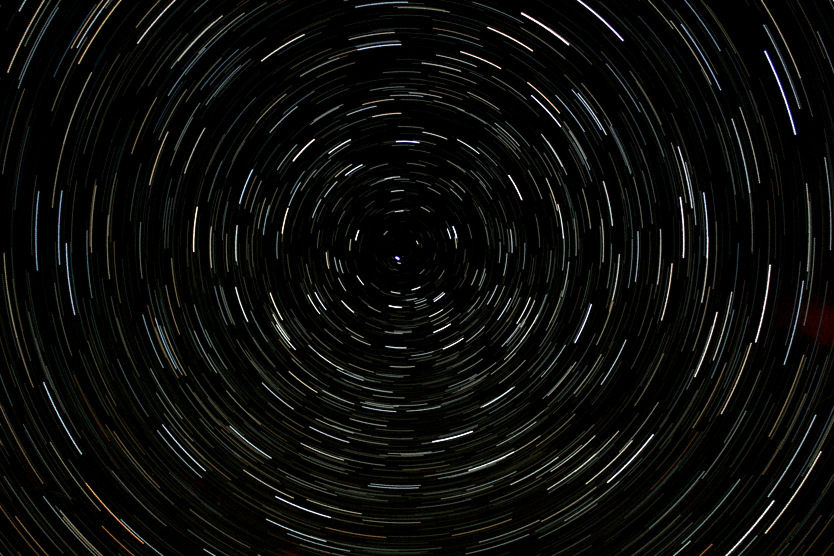
\includegraphics[width=\columnwidth]{img/star_trails_small.jpg}%
  \caption[Star motion around the northern celestial pole.]{Star motion
around the northern celestial pole. The image is com\-po\-sed of se\-ve\-ral
sub-frames, the total exposure time is about half an hour. Image by Robert
Vanderbei \citenum{Vanderbei:2012:LaPalma}.}
  \label{fig:star-trails}
\end{marginfigure}
\margincite{Vanderbei:2012:LaPalma}

\lettrine{O}{ur planet} is rotating, performing one full turn relative to the
sky in a stellar day of about 23 hours and 56 minutes
\cite[\ts12.2]{Allen:2000:Allen}. This poses a problem to photographers: Due to
the low light intensity of most astronomical objects, the exposure times for
astronomical images range from seconds to several hours. Without counteracting
the Earth's rotation, the stars travel long distances across a camera's image
sensor during exposure. Figure~\ref{fig:star-trails} shows an intentional
example of this effect.

Efforts to tackle this problem have lead to the development of specialized
mechanical devices, actuated \emph{telescope mounts}, that follow the stars'
motion. However, mechanical devices are never perfect. A slight imperfection in
the shape of a cog or a worm in the gear of a telescope mount leads to pointing
errors of usually several arcseconds\footnote[][3mm]{One arcsecond (\as) is the
3600$^\text{th}$ fraction of a degree.}. Taking into account the fine angular
resolution of typical imaging setups, this means several pixels of blur during a
long-exposure image.

The periodic error correction method based on Gaussian processes
(Chapter~\ref{ch:periodic-error-correction}) is suitable to address periodic
errors in telescope tracking. In this chapter we first describe the telescope
guiding problem (Section~\ref{sec:problem-statement}), and then apply the method
on both simulation and hardware experiments (Section~\ref{sec:pec-experiments}).

\section{The Telescope Problem}
\label{sec:problem-statement}

\begin{marginfigure}
\centering%
\footnotesize%
  \begin{tikzpicture}%
    \node [draw=none, inner sep=0] (t)
{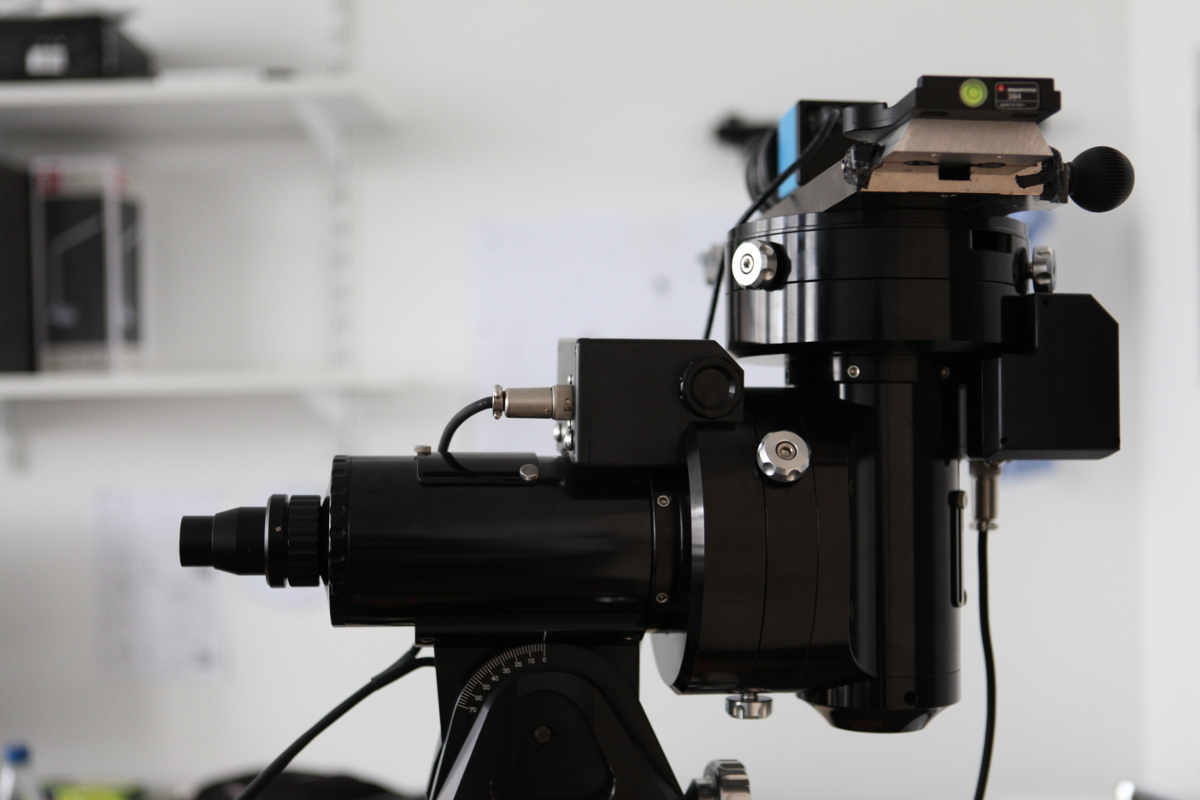
\includegraphics[width=\columnwidth]{img/equatorial_mount.jpg}};
    \draw [dgr, line width=1pt, transform canvas={yshift=-5.8mm}]
    (t.west) -- node[above, text=white]{RA} (t.east);
    \draw [dgr, dashed, line width=1pt, transform canvas={xshift=11.5mm}]
    (t.north) -- node[right, text=white]{Dec} (t.south);
  \end{tikzpicture}%
  \caption[Typical German equatorial mount.]{Typical German equatorial
mount. When used for astronomical imaging, the right ascension (RA) axis is
aligned with the Earth's rotational axis. The declination axis (Dec) is
necessary to be able to point at arbitrary
positions.}
  \label{fig:equatorial-mount}
\end{marginfigure}

Amateur telescope mounts for astronomical imaging are usually built in
equatorial design \margincite{Parker:2007:Making}%
\margincite{Beish:2001:Design}\citenum{Parker:2007:Making, Beish:2001:Design},
one such mount is shown in Figure~\ref{fig:equatorial-mount}. The mechanics is
designed in a way that the right ascension (RA) axis of the telescope mount is
aligned with the Earth's rotational axis when set up properly. This way, only
this axis has to be constantly in motion to follow the stars, which simplifies
the control problem. The telescope can now be modeled in the form of a linear
scalar model
\begin{align}
\label{eq:telescope-problem}
  \dot x(t) &= a_cx(t) + b_cu(t) + g(t),
\end{align}
where $a_c$ is the scalar dynamics, $b_c$ the scalar input gain and $g(t)$ a
scalar disturbance. As described in detail in
Chapter~\ref{ch:periodic-error-correction}, the disturbance is modeled with a
quasiperiodic Gaussian process regression model. It should be noted that in
practice, measurements of $\dot x(t)$ are generally not available and will be
approximated numerically, see also the experimental details in
Section~\ref{sec:pec-experiments}.

Existing \emph{periodic error correction} systems require careful system
identification by the user of the telescope, and still regularly lead to
unsatisfactory performance.

A challenge specific to this astronomical application is that state
measurements are performed by taking images of guiding stars
\margincite{Parker:2007:Making}\citenum[\ts1]{Parker:2007:Making}, which
requires relatively long exposure times, resulting in the measurement interval
reaching the order of magnitude of the error periodicity. This is precisely the
domain in which we expect to see utility from a periodic model.

The performance gain one can expect from the use of a periodic model for
feed-forward compensation depends on the sampling rate of the control system:
If the external error is slow compared to the measurement rate, a locally
linear model is sufficient. But if the external error is on the same time scale
as the measurement, it helps to use feed-forward control based on GP
predictions. With the presented approach it is even possible to choose the
control interval smaller than the actual measurement interval. See
Section~\ref{sec:pec-simulation} for a more detailed discussion.

\section{Experiments}
\label{sec:pec-experiments}

The presented method  was implemented for the telescope problem and evaluated
on different problems. After testing on a simulated telescope system, where the
performance under different measurement frequencies and under sensor failure was
analyzed, the proposed method was evaluated in an experiment on a real
telescope system, showing substantial improvements in control performance.

\subsection{Simulated System}
\label{sec:pec-simulation}

The period length of the periodic error in telescopes is relatively long. To
allow rapid prototyping, we designed a simulation system with dynamics similar
to a real telescope. Experiments have shown that the model can be simplified by
considering only the angular pointing error as state, measured relative to the
desired state. The pointing error can be influenced by an input velocity.
The resulting model is
\begin{equation}
  \dot x(t) = u(t) + g(t),
\end{equation}
with an unknown function $g(t)$ that is observed to be quasiperiodic.

Figure~\ref{fig:error_vs_dt} shows simulation results that empirically confirm
the intuition from Section~\ref{sec:problem-statement} that the benefit of
periodic prediction in control depends on the sampling rate. Using the numerical
simulation, we compare, for various sampling rates of the state,
\begin{itemize}
\item an MPC controller using the linear model
\eqref{eq:problem} with \mbox{$g(t) = 0\quad \forall t$}
\item two MPC controllers, both using a nonparametric, but fully stationary
(i.e.\ not periodic) GP model for $g$ with the square exponential covariance
function \eqref{eq:square-exp}; one of these models uses a length scale smaller
than the periodicity (\ie it can extrapolate periodic swings locally, but not
beyond one period); the other a length scale longer than the periodicity (\ie it
averages over the periodic variations)
\item two MPC controllers using instances of the periodic model for $g$; one in
which the hyperparameters are fixed to a good value a priori (amounting to the
assumption that the period of $g$ is known), the other using the full setup
described in Section~\ref{sec:gps_for_quasiperiodic_functions}, in which the
periodicity hyperparameter is learned by type-II maximum likelihood during
identification
\end{itemize}
Since we are only interested in the performance in the limit in this experiment,
all the controllers were run for an identification phase of 10 period lengths
to avoid artifacts from identification.
Figure~\ref{fig:error_vs_dt} shows RMS error, i.e.\ deviation of the state from
the origin, as a function of the sampling time. The RMS error is measured over
10 period lengths, starting after the identification phase. The discretization
time for the MPC is always set to \nicefrac{1}{100} of the period length, \ie to
1\unit{s}. Between measurements, the MPC controllers are operated in open-loop
mode, i.e. the control actions are obtained from the sequence of the last MPC
optimization.

\begin{figure}
\centering%
\footnotesize%
\inputTikZ{error_vs_dt_fine}%
\caption[Comparison of the RMS error at different sampling times.]{Comparison
of the RMS error at different sampling times (in simulation), for five different
prediction models: linear (\ref*{p:edt-lin}), square exponential with $\ell \ll
\lambda$ (\ref*{p:edt-se-short}), square exponential with $\ell \gg \lambda$
(\ref*{p:edt-se-long}), periodic with inferred $\lambda$ (\ref*{p:edt-per-inf})
and periodic with optimal $\lambda$ (\ref*{p:edt-per-opt}).
MPC control inputs are computed at the indicated sampling times, shown as a
fraction of the period length. The control rate is 1\unit{Hz} for every plot.
The MPC parameters were set to $\SC=10^2$ and $\CC=10^1$. The horizon length was
chosen such that the horizon covers the time until the next measurement.
Between measurements, the MPCs are operated in open-loop mode. $g(t)$ is set to
be a sine with fixed period $\lambda = 100\unit{s}$. }
\label{fig:error_vs_dt}
\end{figure}

The results demonstrate the intuition: For sampling times much smaller than
$\lambda$, the dynamics are locally linear, and all models achieve an error
close to zero. Their performance difference is only marginal (lower left in
Figure~\ref{fig:error_vs_dt}). For sampling times between about 10\unit{\%} and
80\unit{\%} of $\lambda$, the periodic model offers considerable benefits. When
the sampling times are close to, or larger than, the periodicity, the Nyquist
rate imposes limits on identifiability of the system, which adversely affects
the performance of the periodic nonparametric model. This shows that a broad
prior can lead to bad performance if only little data is available. On the
other hand, if $\lambda$ is known precisely, very good control is possible even
for sampling rates lower than $\lambda$. The parameter-inferring model
(\ref*{p:edt-per-inf}) in Figure~\ref{fig:error_vs_dt} represents the
performance of a system almost ignorant of $\lambda$ in the beginning: the
prior is very broad. One can expect prior information about $\lambda$ of
varying vagueness to give performance somewhere in the region between the
parameter-inferring model (\ref*{p:edt-per-inf}) and the optimal-parameter
model (\ref*{p:edt-per-opt}) in Figure~\ref{fig:error_vs_dt}.

The case where sampling rate and $\lambda$ are equal is special, since then $g$
appears to be constant in the measurements, and even the informed periodic
model can not learn the behavior of $g$. A weaker version of this effect is also
visible in the plot at a sampling rate of $\nicefrac{\lambda}{2}$. This
``selection bias'' affects all regression models, including the aperiodic ones.

\subsection{Evaluation of Fault Tolerance}
\label{sec:fault_tolerance}

A similar experiment was conducted to investigate the effect of missing
measurements on the performance of the controlled system.
Figure~\ref{fig:error_vs_darkness} shows the empirical results. The setup is the
same as in the experiment described before, but now the sampling time is fixed
to a value of $5\unit{s}$, while the period length is $100\unit{s}$. The length
of the horizon is set to $41$ time steps (\ie 205\unit{s}), covering more than
two full periods of the periodic effect, which is a realistic setting for a real
telescope.

After giving the system enough time to learn under regular output measurements,
no new data is used to update the GP model of $g(t)$, and no new state estimate
is available to the controller. This corresponds to a fault in the sensor (or
clouds in front of the camera in the telescope setting). The sensor does not
recover within the simulation time. Figure~\ref{fig:error_vs_darkness} shows
the performance of the different controllers, measured in terms of the RMS
error since the beginning of the fault, here at time $0$. In all controller
setups, the MPC control sequence can not be updated as there is no state
estimate available. For the following time steps without measurement, the MPC
therefore is operated in open-loop mode, \ie the control actions from the
control sequence computed at the time before the fault are used.

At the beginning of the failure (lower left of
Figure~\ref{fig:error_vs_darkness}), the performance of all methods is good,
since the effect of the periodic disturbance is still small. Over time, we see
the simple controller without prediction (\ref*{p:edt-lin}) slowly degrading.
Interestingly, the performance of the GP with square exponential kernel with
too long a length scale (\ref*{p:edt-se-long}) performs even worse than not
predicting $g(t)$ at all. This illustrates how critical the choice of the
hyperparameters is and that a wrong choice can even degrade the performance.
The model with sensible length scale (\ref*{p:edt-se-short}) performs
significantly better initially, but the extrapolation of the SE kernel degrades
quickly (see also Figure~\ref{fig:kernels} (a)) resulting in an overall
performance that is only slightly better than for the linear model.

With periodic predictions, in contrast, the controllers perform significantly
better during the fault. The periodic GP (\ref*{p:edt-per-inf}) is better than
the SE with short length scale, even if the period length is inferred and not
fixed at a good value. The RMS error for the GP with optimal parameter
$\lambda$ (\ref*{p:edt-per-opt}) is virtually zero and even a controller having
access to the true function $g(t)$ would therefore only show marginal
improvement. This analysis shows that the proposed combination of a periodic GP
model and MPC control is able to compensate temporary sensor failures and
maintain high control performance for locally periodic dynamic effects.

\begin{figure}%
\centering%
\footnotesize%
\inputTikZ{error_vs_darkness}%
\caption[Comparison of the RMS error after sensor failure.]{Comparison of the
RMS error after sensor failure (in simulation), for five different prediction
models: linear (\ref*{p:edt-lin}), square exponential with $\ell \ll \lambda$
(\ref*{p:edt-se-short}), square exponential with $\ell \gg \lambda$
(\ref*{p:edt-se-long}), periodic with inferred $\lambda$ (\ref*{p:edt-per-inf})
and periodic with optimal $\lambda$ (\ref*{p:edt-per-opt}). Sampling time and
discretization time of the MPC are both 5\unit{s}. The MPC parameters are set to
$\HL=41$, $\SC=10^2$ and $\CC=10^1$. After a training period, no new
measurements are available (``dark phase''). The MPC is operated in open-loop
mode. $g(t)$ is set to be a sine with fixed period $\lambda=100\unit{s}$.}
\label{fig:error_vs_darkness}
\end{figure}

\subsection{Hardware Experiment}
\label{sec:hardware}

We have tested our implementation on a physical system, a commercially
available \emph{Vixen} Sphinx telescope mount (Figure~\ref{fig:hardware}).
Without closed-loop control, this mount shows about 7\as~of RMS error after
correction for static drift. The error arises from the imperfect shape of the
cogs in the gear of this mount (Figure~\ref{fig:gearbox}). The imperfect shape
is not visible to the naked eye, see Figure~\ref{fig:hardware_measurement} (a)
for an uncontrolled measurement.

Because outdoor measurements are subject to random, time-varying effects like
weather conditions, we constructed a more reproducible experimental setup using
a second, high-precision gearless \emph{ASA} DDM60
\clearpage

\begin{figure}
\centering%
\footnotesize%
  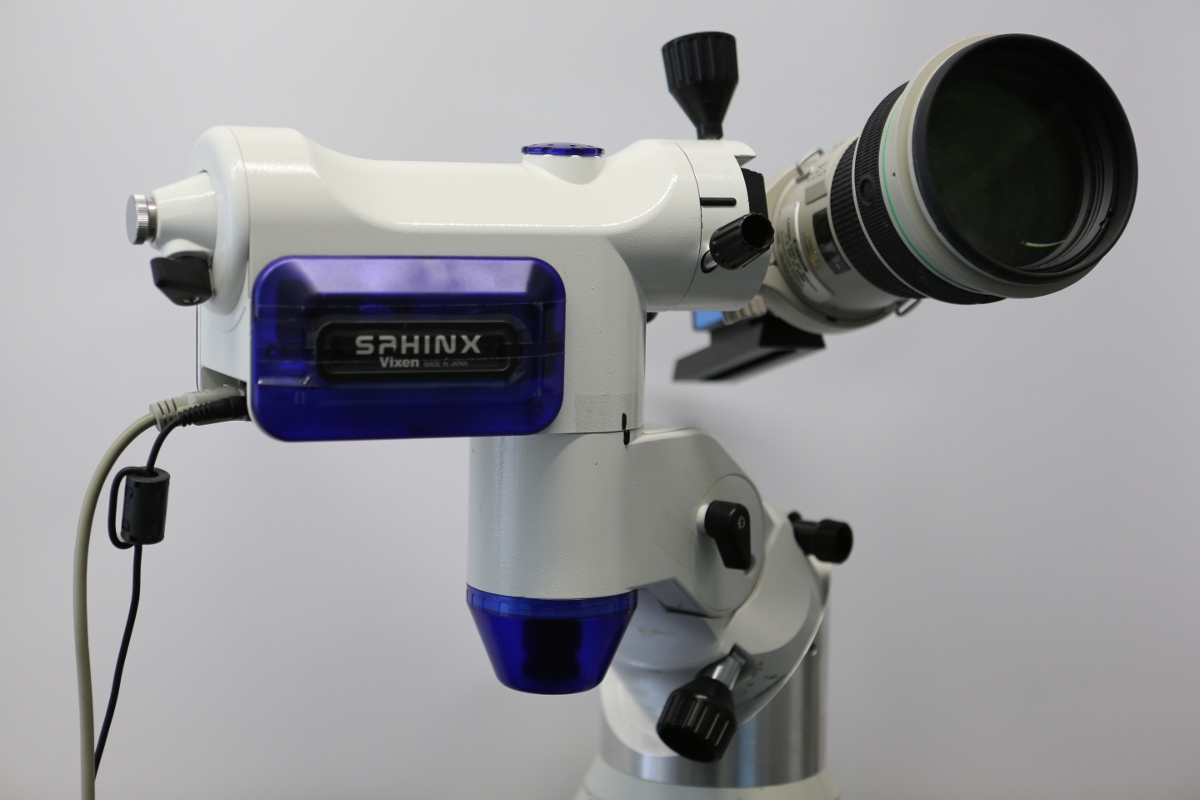
\includegraphics[width=\columnwidth]{img/mount_1200.jpg}%
  \caption[The telescope mount used for the tracking experiments.]{The telescope
mount used for the tracking experiments. On the right side is the camera lens
used as guiding telescope. A main telescope is not used for the tests.}%
  \label{fig:hardware}%
\end{figure}

\begin{figure}
\centering%
\footnotesize%
  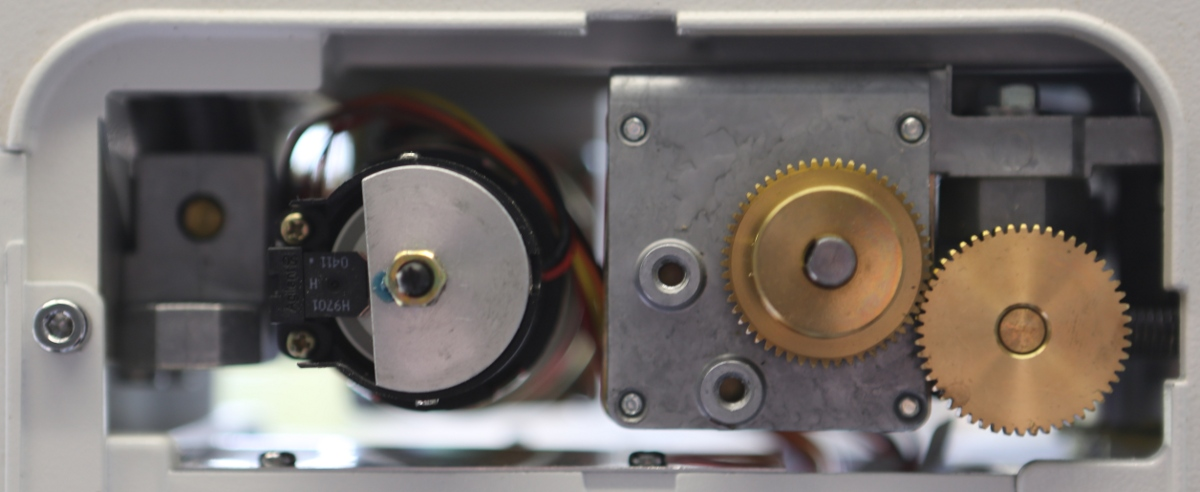
\includegraphics[width=\columnwidth]{img/gearbox_1200.jpg}%
  \caption[The gearbox of the telescope mount.]{The gearbox of the telescope
mount. One of the motors is visible on the left. The two cogs on the right
transmit the motor's rotation to a worm gear (not visible), which sits on the
same axis and thus has the same period. These cogs and the worm gear are the
likely
source of the periodic error.}%
  \label{fig:gearbox}%
\end{figure}

\noindent Pro telescope mount equipped
with a laser ``star'' as tracking reference (Figure~\ref{fig:gearless-mount}).
It has a typical tracking RMS error of about 0.4\as. The measurement is done
with a \emph{Canon} EF400DO lens on a \emph{The Imaging Source} DMK
41AU02.AS camera.

\begin{marginfigure}[3cm]
\centering%
\footnotesize%
  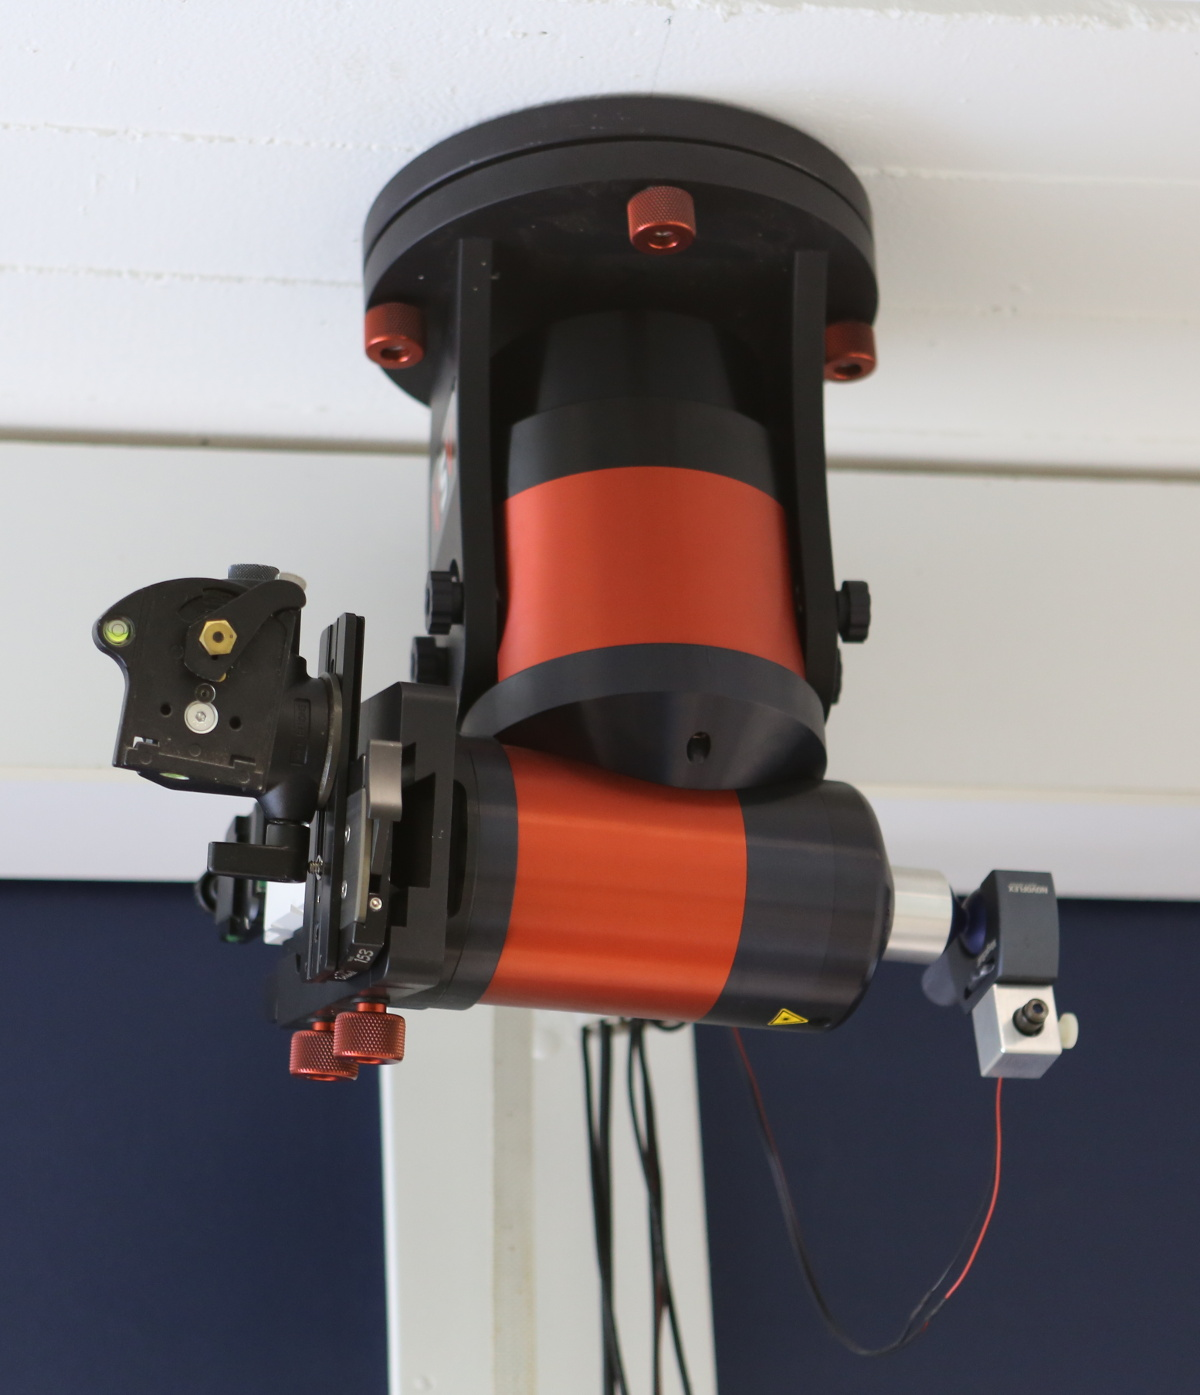
\includegraphics[width=\columnwidth]{img/mount_ceiling_1200.jpg}%
  \caption[The gearless \emph{ASA} DDM60 Pro telescope mount.]{The gearless
\emph{ASA} DDM60 Pro telescope mount, attached to the ceiling of our
laboratory.}%
  \label{fig:gearless-mount}%
\end{marginfigure}

For the hardware interaction, the open source ``PHD Guiding'' software package
is used. In the original implementation this software uses a proportional
controller with hysteresis to prevent direction switching. The telescope is
connected to the computer with a \emph{Shoestring Astronomy} GPUSB, a
device that sends pulse-width modulated signals to telescopes over a commonly
used 6-wire interface.

We altered the software to gain access to the measured displacement of the
camera image. The value is sent through a network socket to \textsc{Matlab},
with which the proposed controller was implemented to calculate the optimal
control signal. The control signal is sent back to the guiding software, which
\footnotetext[2]{The pixel resolution of our lens and camera
combination was determined with \texttt{nova.astrometry.net}
\citenum{Hogg.ea:2008:Automated}.}%
\margincite{Hogg.ea:2008:Automated}%
then passes it on to the telescope hardware. For plotting and
calculation of the RMS error, the measured displacement is converted from
pixels into arcseconds (\as) with an empirically determined conversion
factor\footnotemark.

For real-time implementation, algorithmic complexity is relevant. The
computational cost of the GP prediction scales cubically in the number of
data points. To bound computational cost, we limit the number of used data
points to 90 in a moving window fashion. This gives a sufficient coverage of
270\unit{s}, or about 3 periods of the short periodic component. Since
inference continuously runs in an extrapolation setting (see also
Figure~\ref{fig:kernels} (b)), this is sufficient for precise inference and
control.

For the prediction of the dynamics in the MPC framework, an ODE-solver is
employed to predict the tracking reference from the mean of the GP prediction.
This has manageable computational cost because the inference of a Gaussian
process is dominated by the initial one-time operation of inverting the Gram
matrix $K$ in $\mathcal{O}(\ND^3)$ time, while evaluating the mean function at
$M$ times only has cost $\mathcal{O}(M\ND)$.

The optimization of the hyperparameters is also an expensive part of this
algorithm. As the kernel Gram matrix has to be filled and inverted at every
evaluation of the objective function, the number of evaluations has to be kept
small at every sampling time. We use a numerical optimizer based on the BFGS
update
\margincite{Broyden:1969:new}%
\margincite{Fletcher:1970:new}%
\margincite{Goldfarb:1970:family}%
\margincite{Shanno:1970:Conditioning}%
\citenum{Broyden:1969:new, Fletcher:1970:new, Goldfarb:1970:family,
Shanno:1970:Conditioning}, a quasi-Newton algorithm that updates an
estimate of the inverse Hessian in each iteration. In the standard
implementation, the estimate of the Hessian obtained at one time step is
discarded after each individual call to the optimizer. For the use in the
control setting, we altered the algorithm so that the estimate of the inverse
Hessian is stored and used to initialize the optimizer's estimate at the next
sampling time. This makes it possible to do one iteration per sampling interval
(in a sense, threading the optimization algorithm into the learning algorithm).
This significantly reduces computation time.

The presented method was tested on two different setups, one with an MPC based
on the linear model only and one with the GP prediction for the periodic error
g(t). The test was run 3 times for 25\unit{min} each. Both the sampling and the
discretization time were set to 3\unit{s}. The horizon length was $\HL=10$; the
state and control weights were set to $\SC=10^2$ and $\CC=10^3$. The results of
these runs are shown in Table~\ref{tab:results-hardware}.

\begin{table}[ht]
{\centering
\footnotesize
\begin{tabular}{@{} r *4{r} @{}}
\toprule
          & Run 1  & Run 2  & Run 3  & {\bfseries Mean}   \\
\midrule
Plain MPC & 0.9839 & 1.0234 & 0.9353 & {\bfseries 0.9809} \\
GP-MPC    & 0.7365 & 0.7792 & 0.7605 & {\bfseries 0.7587} \\
\bottomrule
\end{tabular}
\vskip 0.1in
\caption[Experimental results from indoor telescope tracking.]{Experimental
results from indoor telescope tracking (RMS error, \as).}
\label{tab:results-hardware}
}
\end{table}

The RMS error drops by 22.64\unit{\%} through the use of GP predictions in this
hardware setup. Baseline measurements without movement showed about 0.25 to
0.35\as~of noise. The noise introduced by the stepper motor could not be
quantified with the current measurement system. Overall, the presented method
eliminated at least a third of the controllable error, after subtracting
baseline noise but without taking the stepper motor into account. This is a
good result in this domain, but could probably be further improved, which is
also visible through the weak residual structure visible in
Figure~\ref{fig:hardware_measurement} (c).

\begin{figure}
\centering
\footnotesize
\subfloat[Uncontrolled, RMS(e) =
6.533\as]{\inputTikZ{measurement_raw}
\label{fig:raw_measurement}}\\
\subfloat[Plain MPC, RMS(e) =
1.023\as]{\inputTikZ{measurement_plain_mpc}
\label{fig:plain_mpc_measurement}}\\
\subfloat[GP-MPC, RMS(e) = 0.779\as]{\inputTikZ{measurement_gp_mpc}
\label{fig:gp_mpc_measurement}}
\caption[State measurements from the indoor tracking experiment.]{State
measurements from the indoor tracking experiment: Without controller
(\refpoints{p:meas-raw}), where the highlighted
area (\ref*{p:meas-zoom}) shows the vertical range of the two other plots; for
plain MPC using only a linear model (\refpoints{p:meas-plain}); and for the
periodic Gaussian process based MPC (\refpoints{p:meas-gp}). The controlled
measurements' data are from run 2 of our experiments, which resulted in the
highest (worst) RMS error for both models (Table~\ref{tab:results-hardware}). }
\label{fig:hardware_measurement}
\end{figure}

Figure~\ref{fig:spectra} shows the power spectra of the measurements,
obtained from the Fourier transform. It is noticeable that the strong periodic
components near 100\unit{s} and near 500\unit{s}, as well as the constant
component are highly damped with the presented method.

\begin{figure}
\centering
\footnotesize
\subfloat[Plain MPC]{\inputTikZ{spectrum_plain_mpc}
\label{fig:spectrum_plain_mpc}}\\
\subfloat[GP-MPC]{\inputTikZ{spectrum_gp_mpc}
\label{fig:spectrum_gp_mpc}}
\caption[Power spectra from the indoor tracking experiment.]{Power spectra of
the measurements of Figure~\ref{fig:hardware_measurement}, plain MPC using only
a linear model (\ref*{p:spec-plain}), and periodic Gaussian process model based
MPC (\ref*{p:spec-gp}).} \label{fig:spectra}
\end{figure}


\section{Conclusion}

Telescope tracking requires high precision with low sampling rates. Therefore,
Gaussian process regression with a quasiperiodic prior is a well-suited
prediction framework for this application.

Numerical and hardware experiments confirm the intuitive result that the benefit
of periodic models depends on the relative size of state sampling and
disturbance frequencies. We showed that, even in cases where the gain of a
periodic prediction is only marginal during normal operation, these models are
beneficial when sensors fail temporarily. The presented method also shows
considerable increases in control performance, confirming the practical utility
of this framework.

\chapter{Software Implementation: PHD2 Guiding}
\label{ch:software-implementation-phd-guiding}

\lettrine{T}{he method} described in Chapters~\ref{ch:periodic-error-correction}
and \ref{ch:predictive-error-correction-for-telescopes} was implemented as part
of the telescope guiding software \emph{PHD2 Guiding} \cite{Stark.ea:2016:PHD2}.
PHD2 Guiding is an open-source telescope guiding software used by many amateur
astronomers. Developing the adaptive periodic error correction algorithm as a
part of PHD2 Guiding makes it possible to reach the astronomers that
already use this software. Also, by using the mature and well-engineered PHD2
Guiding platform, we do not need to take care of hardware interactions and can
instead focus on the guiding algorithm itself.

After introducing the PHD2 Guiding framework
(Section~\ref{sec:phd2-guiding-framework}), we describe several modifications
to the algorithm (Section~\ref{sec:algorithm-changes}). These changes were
necessary to increase robustness for the use by unexperienced users.
We then briefly present a guiding method for the second telescope axis
(Section~\ref{sec:the-dec-axis}) before discussing the results of experiments
with this predictive telescope guiding framework
(Section~\ref{sec:phd-guiding-experiments}).

\section{The PHD2 Guiding Framework}
\label{sec:phd2-guiding-framework}

PHD2 Guiding is a GUI-based software for telescope guiding optimized for
easy usage. Figure~\ref{fig:PHD2} shows the main window of the software with
star display and residual error curves. The software includes drivers for many
guiding cameras as well as telescope mounts, and handles the hardware
interactions. PHD2 Guiding is open-source software, so it is possible to
integrate additional features. It is under active development and is downloaded
several thousand times per month.

The current state-of-the-art guiding algorithm in PHD2 Guiding is a
proportional controller with hysteresis to prevent changes in the control
direction. This algorithm does not make use of extrapolation. The lack of a
predictive control scheme results in residual structure in the pointing error
when the sampling frequency is low. It is also not robust, \eg when a cloud
occludes the guide star for some time. In such a case the guide star is
usually lost because it moved too far away from its original position during the
period without measurements.

These two issues can be tackled with the GP framework: Structured extrapolation
together with predictive control reduces residual error and residual structure.
Also, since extrapolation and predictive control still offer a control input
even when no measurements are available, it is possible to issue control actions
in those cases. This results not only in a decrease in pointing error, but also
increases robustness because the guide star remains closer to the target
position.

\begin{figure}
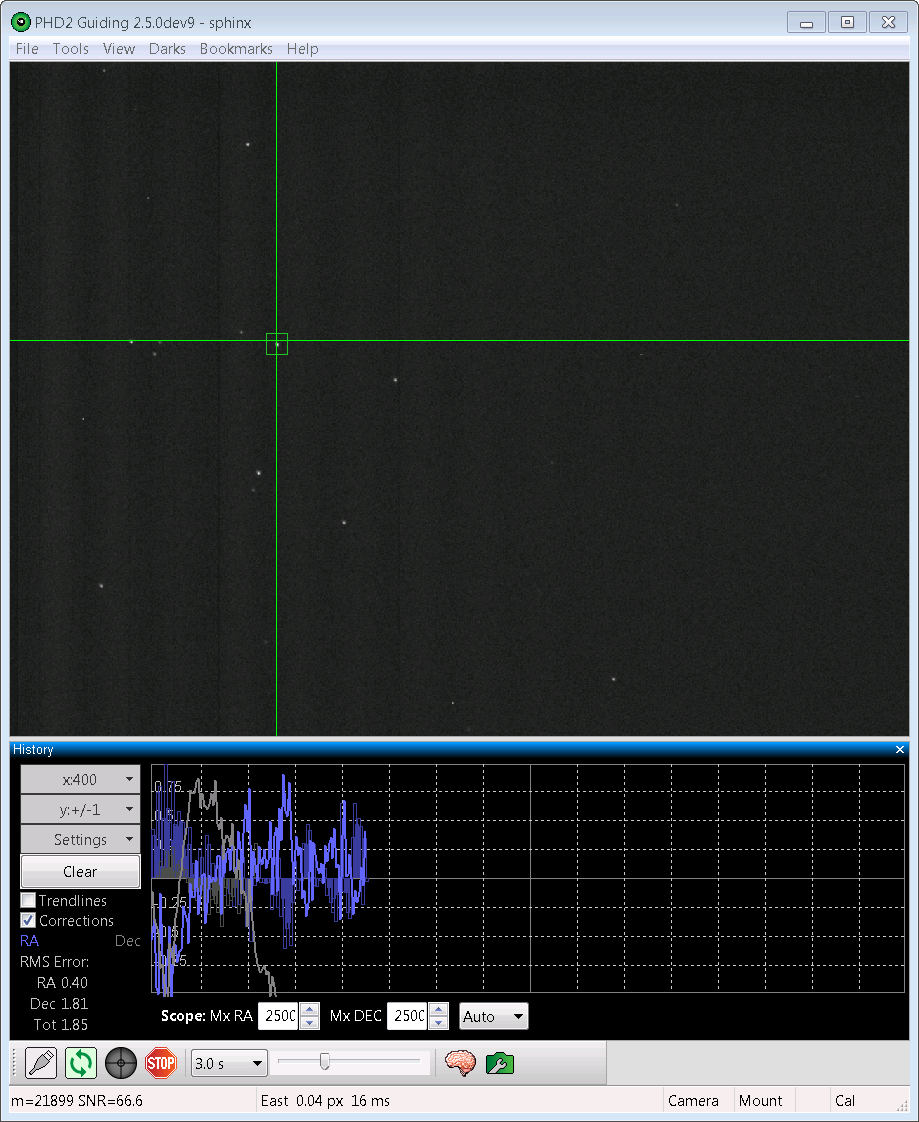
\includegraphics[width=\textwidth]{img/PHD2_screenshot_crop.png}
\caption[GUI of PHD2 Guiding in version 2.5.0.]{GUI of PHD2 Guiding in
version 2.5.0. The upper part is the star display with the guide star
highlighted by the crosshair. The search region for the guide star is the small
box. The lower part shows the residual error curves and the controls.}
\label{fig:PHD2}
\end{figure}

\section{Periodic Error Correction for PHD2 Guiding}
\label{sec:algorithm-changes}

Despite the fact that there are libraries for Gaussian processes in C++, we
chose to implement the GP algorithm ourselves. This decision was made because
some crucial features, such as the conditioning on a subset of the kernel
combination, are missing in the readily available libraries.

Much of the GP infrastructure is based on linear algebra. Thus, we selected to
use the Eigen matrix library \cite{Guennebaud.Jacobs.ea:2010:Eigen} to make
use of fast and well-tested linear algebra code. Using the Eigen library also
increases the readability of the overall implementation. The Eigen library
itself has no external dependencies and is therefore relatively easy to include
in the existing project.

\subsection{Data Acquisition}

Instead of retaining all collected data, it is necessary to limit the number
of data points to keep the computational effort bounded and the runtime
predictable. We use a FIFO buffer to store data points, where, once the buffer
is full, the oldest entry is dropped whenever a new data point is added. This
amounts to a windowing of the dataset.

Using the measured pointing error directly to identify the dynamics function
turned out to be not robust enough during our intensive testing. Therefore, we
model the \emph{accumulated} gear error
\begin{equation}
  \label{eq:accumulation-model}
 a_{k} = e_k + \sum_{i=0}^{k-1} u_i
\end{equation}
where $e_k$ is the measured pointing error at time step $k$ and $u_i$ are the
control signals at time $i$. This model is more robust because the error
introduced by the gear accumulates, while random effects caused by, \eg
the stepper motor, average out. Overall, this leads to a better
signal-to-noise ratio for the accumulated gear error compared to the absolute
pointing error.

Additionally, the measurement process does not have uniform noise. Since the
location of the guide star is determined from pixel intensities via a weighted
centroid of the star's pixels, the accuracy of the centroid calculation depends
on the signal-to-noise ratio (SNR) of the image. In PHD2 Guiding, the SNR is
calculated according to the method described by
\textcite{Simonetti:2004:Measuring}; the relation between the SNR and the
measurement noise variance was determined empirically and modeled by the linear
regression model
\begin{equation}
  \sigma(\rho) = w_{\sigma,1}(\rho - \rho_0)^{-1} + w_{\sigma,0},
\end{equation}
where $\rho$ is the SNR, $\rho_0$ is an input offset and $w_{\sigma}$ are the
parameters for the regression model. Figure~\ref{fig:snr-vs-sigma} shows this
relationship and the data used to determine it.

\begin{marginfigure}
\footnotesize
\setlength{\figurewidth}{0.8\textwidth}%
\setlength{\figureheight}{0.6\textwidth}%
\inputTikZ{snr_vs_sigma}
\caption[Relationship between the signal-to-noise ratio and measurement
variance.]{Relationship between the signal-to-noise ratio and measurement
variance. Shown are RMS errors from simulated exposures for different SNRs
(\ref*{p:snr-sig}) and the regression line (\ref*{p:snr-sig-reg}).}
\label{fig:snr-vs-sigma}
\end{marginfigure}

The value of the estimated noise variance is stored along with the measurements
of the signal. It is then used in a heteroscedastic noise model, as described in
Section~\ref{sec:heteroscedastic-noise}.

\subsection{Modeling}

\begin{figure}
\footnotesize
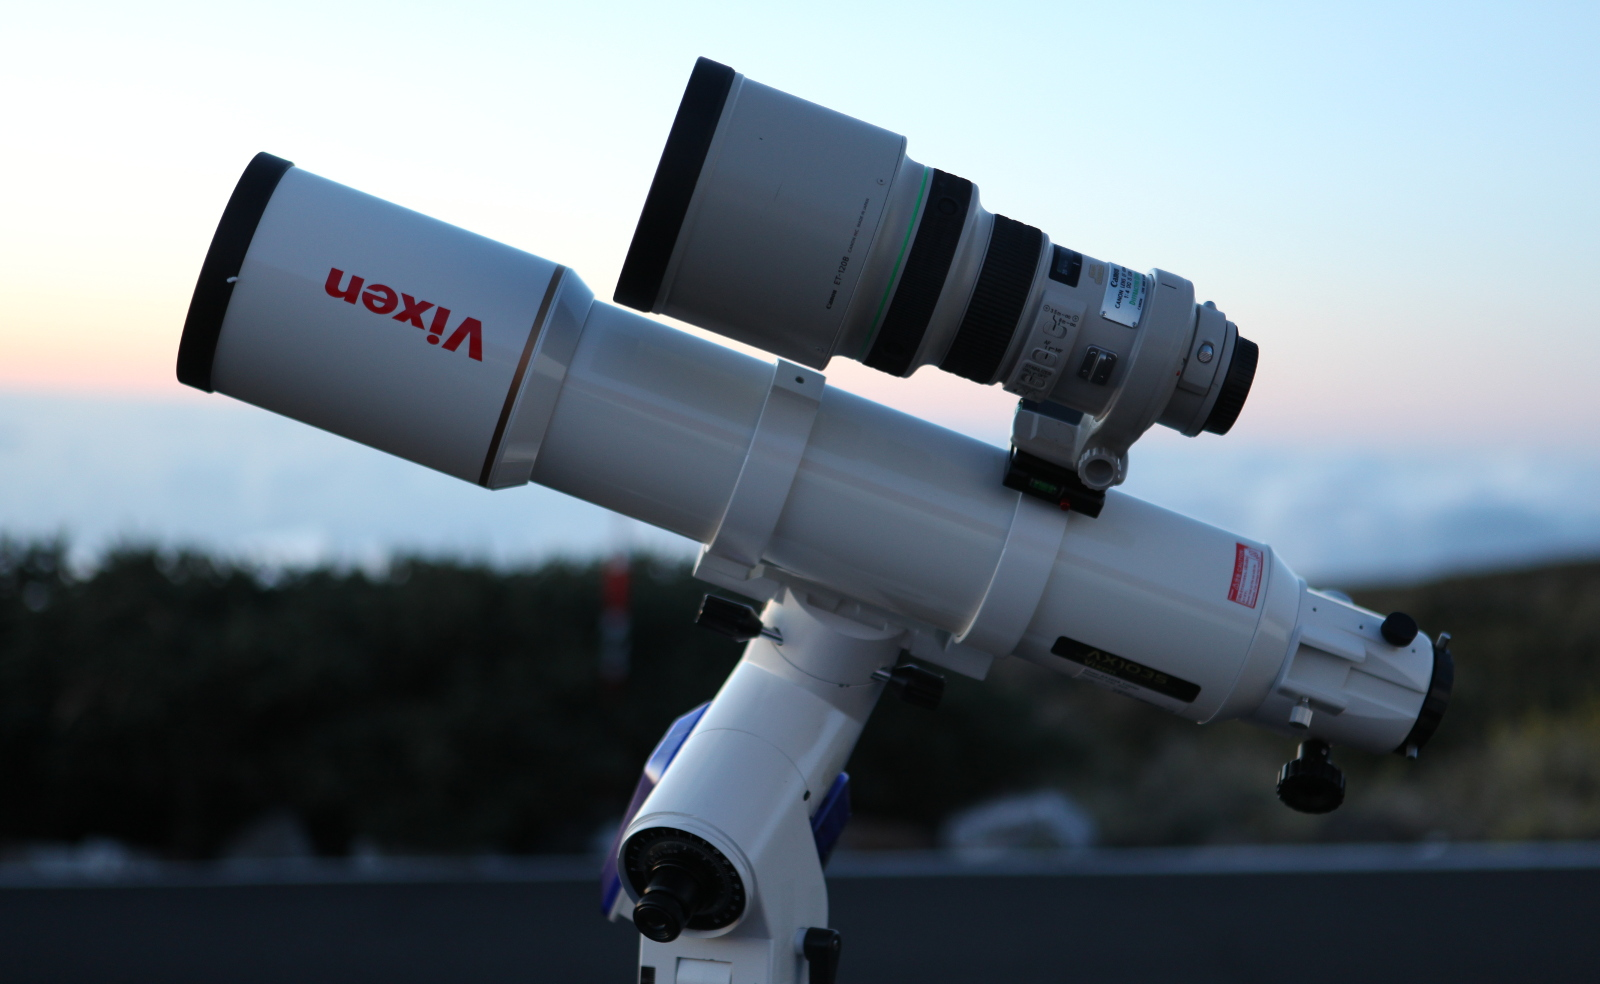
\includegraphics[width=\textwidth]{img/telescope_small.jpg}
\caption[Telescope setup with main and guiding telescope.]{Telescope setup with
main and guiding telescope. The guiding telescope is mounted ``piggyback'' on
the main imaging telescope. The cameras are not yet attached.}
\label{fig:typical-setup}
\end{figure}

In real astronomical imaging setups (see Figure~\ref{fig:typical-setup}
for an example), it is almost impossible to align the axis of the telescope
mount with the Earth's rotational axis perfectly. Thus, in most cases there will
be a moderate drift that needs to be modeled and predicted in addition to the
periodic component. As it is hard to find the linear drift component
independently of the periodic gear error, we employ a joint model as described
in Section~\ref{sec:explicit-feature-functions}, consisting of fixed features
for constant and linear components and a Gaussian process to model the nonlinear
part:
\begin{equation}
 a(t) = [\beta_0\q \beta_1]
  \begin{bmatrix}1\\t\end{bmatrix} + f(t)
\end{equation}
with $f(t)\sim\GP$. We assume an uninformative prior where $\beta\sim\N(0,B)$,
$B\inv\to 0$, as detailed in \cite[\ts2.7]{Rasmussen.Williams:2006:Gaussian}.

The GP itself consists of three different components that were identified
during experimentation. It is also possible to automatically identify kernel
components \cite{Duvenaud.Lloyd.ea:2013:Structure}, but for this application
the hand-crafted kernels were more compact and robust. The different components
are:
\begin{description}
  \item[slowly-varying SE] Not all mechanical effects are periodic.
    In order to allow for mechanical deviations, \eg deformations due to load
    shift in the mechanics, we include a long-length-scale square exponential
    kernel. As a result of the long length scale, this part of the model is
    also amenable to extrapolation.
    \begin{equation}
      \k_{\mathsc{se},0}(t, t'; \theta_0, \ell_0) = \theta^2_0
      \exp\left(- \frac{|t-t'|^2}{2\ell^2_0}\right)
    \end{equation}
  \item[periodic] The periodic component is the important part of the model. It
    captures the recurrent disturbances from the gear. This component was chosen
    to be periodic to enable long-term predictions.
    \begin{equation}
      \k_\mathsc{p}(t,t';\theta_\mathsc{p},\ell_\mathsc{p},\lambda) =
      \theta^2_\mathsc{p}
      \exp\left(-\frac{2\sin^2\left(\frac{\pi}{\lambda}
      (t-t')\right)}{\ell^2_\mathsc{p}}\right)
    \end{equation}
  \item[quickly-varying SE] Since the actual data is not perfectly periodic, we
    allow for fast variations with a square exponential kernel with short
    length-scale. This kernel captures deviations due to mechanical
    roughness.
    \begin{equation}
      \k_{\mathsc{se},1}(t, t'; \theta_1, \ell_1) = \theta^2_1
      \exp\left(-\frac{|t-t'|^2}{2\ell^2_1}\right)
    \end{equation}
\end{description}

The combined kernel function is the sum of the three individual kernel functions
\begin{fullwidth}\vspace{-\baselineskip}
\begin{equation}
  \label{eq:compund-kernel}
  \k_\mathsc{c}(t,t';\boldsymbol{\eta}) =
\k_{\mathsc{se},0}(t,t';\theta_0,\ell_0) +
\k_\mathsc{p}(t,t';\theta_\mathsc{p},\ell_\mathsc{p},\lambda) +
\k_{\mathsc{se},1}(t,t';\theta_1,\ell_1),
\end{equation}
\end{fullwidth}
where we have subsumed parameter dependencies into the parameter vector
$\boldsymbol{\eta}=[\theta_0, \ell_0, \theta_\mathsc{p},\ell_\mathsc{p},
\lambda, \theta_1, \ell_1]$.
A sample from the compound model, combining the linear part and the GP with
kernel function \eqref{eq:compund-kernel} is shown in
Figure~\ref{fig:model-components}.

\begin{figure}
\footnotesize%
\setlength{\figurewidth}{\textwidth}%
\setlength{\figureheight}{0.6\textwidth}%
\inputTikZ{model_components}%
\caption[Combining the components of the model.]{Combining the components
of the model: Linear drift (\ref*{p:mod-lin}), plus long
length-scale SE (\ref*{p:mod-se}), plus periodic (\ref*{p:mod-se-per}), plus
short length-scale SE (\ref*{p:mod-se-per-se}). One sample of the model is
generated from the individual components.}
\label{fig:model-components}
\end{figure}

The overall model is expressive enough to capture the different aspects of
the problem. While linear drift, slowly-varying SE and the periodic
component are features that can be extrapolated, the quickly-varying SE can not.
It regresses back to the mean quickly after the last data point,
which disturbs the controller. Therefore, while inference is done with the
full model, the predictions are conditioned on the model without the
quickly-varying SE. See Section~\ref{sec:output-projections} for the
details on the output conditioning.

\subsection{Hyperparameter Identification}

While many of the hyperparameters included in the model can be estimated by
mechanical considerations without affecting performance too much, one
parameter can not: the period length $\lambda$. It is crucial for the predictive
power that this parameter closely matches the mechanical period length; there
is little robustness regarding the choice of this parameter.

Instead of relying on the maximization of a probabilistic criterion, the
identification of the main periodic component is done with classic spectrum
analysis. After subtraction of a polynomial fit of order 1 to remove the linear
trend, a Hamming window \cite[\ts7.2.1]{Oppenheim.ea:1999:Discrete} is applied
to reduce spectral leakage effects due to the finite-length signal.

In order to obtain the spectral density of the measured signal, the discrete
Fourier transform (DFT) \citenum[\ts8.1]{Oppenheim.ea:1999:Discrete} is
calculated on the preprocessed data
\begin{equation}
  \label{eq:DFT}
  s_k = \sum_{n=0}^{N-1} a_n e^{-\frac{2\pi \imath}{N} nk},
\end{equation}
where $\mathbf{s}=[s_0, \dots, s_{N-1}]$ is the spectrum, $\mathbf{a}=[a_0,
\dots, a_{N-1}]$ is the data and $\imath$ is the imaginary unit. The period
length of the strongest frequency component is subsequently calculated from the
power spectrum $\mathbf{s}$. In order to ensure constant frequency resolution,
the data vector is zero-padded up to the maximum number of data points in the
FIFO buffer.

In the software implementation, we use the fast Fourier transform (FFT)
\margincite{Gauss:1866:Theoria}\margincite{Cooley.Tukey:1965:Algorithm}
\citenum{ Gauss:1866:Theoria, Cooley.Tukey:1965:Algorithm}
for the spectrum analysis, since the na{\"i}ve
implementation of \eqref{eq:DFT} is not viable for the online use.

\subsection{GP Approximation}

It is important to note that in the case of periodic covariance functions, it
is not enough to do a simple windowing because it is necessary to cover
multiple periods with the data for decent predictive performance. Depending on
the choice of sampling frequency, it is often too expensive to use a full
dataset of consecutive measurements to cover multiple periods. Instead, the
FIFO buffer holds multiple periods worth of measurements and we use a
subset-of-data (SD) approximation to keep inference cheap. See
Section~\ref{sec:subset-of-data} for the details of the SD method.

The fact that the extrapolation position is known in advance is beneficial in
this case. In order to obtain a computationally cheap method, we use the
covariance between the prediction point and the data to select the data points
for the approximation:
\begin{equation}
  \mathbf{x}_\mathsc{sd} = \mathtt{sort}\left\{\mathbf{x}; \k(
\mathbf{x},x)\right\}_{0:M-1},
\end{equation}
where $\mathbf{x}_\mathsc{sd}$ is the selected dataset, $\mathtt{sort}$ sorts
the data $\mathbf{x}$ according to the values of the covariance vector $\k(
\mathbf{x},x)$ and $\{\cdot\}_{0:M-1}$ selects the first $M$ elements.

For each control step, we select a new subset from the large dataset in the FIFO
buffer, depending on the current prediction point. This way we make sure that
there is always relevant data from past periods available to the GP, while
keeping the inference cost low.

\subsection{Control}

The control algorithm used in the guiding software was designed to avoid the
problems that arise from the low sampling frequency, while keeping the
complexity of the algorithm low. Ideally, one would implement an optimal
control scheme as introduced in Section~\ref{sec:control}, but for the
simplicity of the algorithm, only a ``deadbeat'' controller\footnote{A deadbeat
controller is a predictive controller that is tuned to eliminate the entire
error in one step, \ie the error-feedback gain is 1.} was considered. Due to
the low sampling frequency and non-uniform sampling intervals, this deadbeat
control often led to overshoots and instabilities. Reducing the control gain, on
the other hand, led to performance loss due to the periodic error.

The implemented algorithm, therefore, is a hybrid controller: Deadbeat control
is applied for the compensation of the periodic error, and proportional control
is used to drive the residual error to zero. The overall control signal at time
$k$ is given by
\begin{equation}
  \label{eq:dead-P}
  u_k = -(\tilde a_{k+1} - \tilde a_{k}) - g_\mathsc{p} e_k,
\end{equation}
where $\tilde a_{k}$ is the mean prediction of the Gaussian process
modeling the accumulated gear error $a_k$, and $g_\mathsc{p}$ is the control
gain for the proportional controller. The structure of this
hybrid control algorithm is shown in Figure~\ref{fig:PEC_controller}.

\begin{figure}%
  \center%
  \inputTikZ{PEC_controller}%
  \caption[Structure of the telescope controller for the RA axis.]{
Structure of the telescope controller for the RA axis. While the residual error
is handled with proportional control, the GP prediction is accounted for in a
deadbeat fashion.}
  \label{fig:PEC_controller}
\end{figure}

\section{The Declination Axis}
\label{sec:the-dec-axis}

When the alignment between the right ascension (RA) axis and the Earth's
rotational axis is not perfect, the offset introduces a linear drift in the
image plane for \emph{both} axes. Therefore, also the declination (Dec) axis
needs to be controlled.

However, since the declination axis is almost still and only needs to
compensate small drift errors, the regression problem is different from the RA
axis: Due to the low signal-to-noise ratio and the small drift, the control
signal of a proportional control often changes its sign. This leads to gear
backlash effects, disrupting even usual robust regression models, such as
$\ell_1$-regression or Huber-regression \cite{Huber:1964:Robust}.

Since the underlying dynamical model is simple, and the estimation only needs to
find a linear drift, we implemented a trimmed mean estimator for the linear
drift:
\begin{equation}
  \Delta \tilde a^\text{Dec}_{k+1} = \frac{1}{k-2n_T}
    \sum_{i=n_T}^{k-n_T-1} \mathtt{sort}\left\{\mathbf{\Delta
a}^\text{Dec}_{1:k}
  \right\}_i,
\end{equation}
where $\mathbf{\Delta a}_{1:k}^\text{Dec}$ is the collection of finite
differences of the accumulated gear errors $a_k^\text{Dec}$ and $n_T$ is the
number of elements to trim on either side. The $\mathtt{sort}$-operator sorts
the collection according to the values, and $\{\cdot\}_i$ selects the $i$-th
element.

The control structure, which is similar to \eqref{eq:dead-P}, is
shown in Figure~\ref{fig:TM_controller}. The estimated drift
$\Delta \tilde a^\text{Dec}_{k+1}$ is corrected for in a deadbeat
fashion, while the error term is driven to zero with a conservatively-tuned PD
controller \cite{Astrom.Hagglund:1995:Theory}.

\begin{figure}%
  \center%
  \inputTikZ{TM_controller}%
  \caption[Structure of the telescope controller for the Dec axis.]{
Structure of the telescope controller for the Dec axis. While the residual error
is handled with PD control, the prediction from a trimmed-mean estimator is
accounted for in a deadbeat fashion.}
  \label{fig:TM_controller}
\end{figure}

\section{Experiments}
\label{sec:phd-guiding-experiments}

The demonstration of the implemented guiding algorithm was done for the
use-case of tracking stars in the night sky (as opposed to the laboratory setup
of Section~\ref{sec:hardware}). The measurements were made in T{\"u}bingen,
Germany, using a \emph{Vixen} Sphinx telescope mount with a \emph{Canon} EF 400
DO IS USM lens and a \emph{The Imaging Source} DMK 41AU02.AS camera, the same
equipment as in the laboratory setup.

\subsection{Guiding Performance}

The performance of GP guiding is shown in comparison to the state-of-the-art
algorithm\footnote{In PHD2 Guiding, the standard algorithm is ``Hysteresis'',
which is a P-controller with hysteresis to prevent gear backlash effects.} that
is used in PHD2 guiding. Figure~\ref{fig:comparison-sota} shows the exemplary
comparison of the two algorithms under otherwise identical conditions. The
angular pointing error between target position of a guide star and its measured
position is plotted over time. It is visible that the GP guiding shows less
residual structure after the initial learning phase (up to around
1000\unit{s}). Since the GP guider starts with zero information, the effect of
learning is visible in the data by the structural change in the error residuals
after 1000\unit{s}.

\begin{figure}
\setlength{\figurewidth}{0.95\textwidth}%
\setlength{\figureheight}{0.4\textwidth}%
\footnotesize
\inputTikZ{comparison_sota}
\caption[Comparison between state-of-the-art tracking
and GP-based tracking.]{Comparison between state-of-the-art tracking
of PHD2 Guiding 2.5.0 (top, \refpoints{p:comp-sota}) and GP-based tracking
(bottom, \refpoints{p:comp-gpg}).}
\label{fig:comparison-sota}
\end{figure}

When analyzing the guiding performance, the initial learning phase has to be
compared separately. We report the mean, standard deviation and RMS error of the
two different algorithms for the different phases. The GP guiding consistently
outperforms the standard algorithm.

\begin{table}[ht]
{\centering
\footnotesize
    \begin{tabular}{l|rrr|rrr|rrr|}
    & \multicolumn{3}{c|}{overall} & \multicolumn{3}{c|}{for $t<1000$} &
      \multicolumn{3}{c|}{for $t>1000$}\\
    & mean & \mathsc{sd} & \mathsc{rms} & mean & \mathsc{sd} & \mathsc{rms} &
      mean & \mathsc{sd} & \mathsc{rms}\\
    \midrule
Hy & 0.357 & 0.968 & 1.031 & 0.427 & 0.917 & 1.010 & 0.331 & 0.985 &
1.039 \\
GP & 0.122 & 0.751 & 0.761 & 0.088 & 0.893 & 0.895 & 0.136 & 0.685 &
0.697 \\
  \end{tabular}
\vskip 0.1in
\caption[Experimental results from outdoor telescope tracking.]{Experimental
results from outdoor telescope tracking (all numbers
in \as). ``Hy'' is the standard ``Hysteresis'' algorithm and ``GP'' is
the GP guiding algorithm developed in this thesis. In addition to the overall
performance, we report the performance for the initial phase ($t<1000$) and for
the later phase ($t>1000$) separately.}
\label{tab:results-stars}
}
\end{table}

\subsection{Dark Guiding}

In order to show the improved robustness under conditions where the measurement
is unavailable for some time, we implemented a dark guiding mode. When there is
no measurement, the guiding is done with the GP predictions alone. This prevents
the telescope from moving away from the guide star too quickly, increasing
chances of finding the guide star after recovery of the measurement process.

Figure~\ref{fig:cloud-tracking} shows the benefit of the GP guider under
occlusion conditions. With the GP guider the linear and periodic motion is
predicted, keeping the pointing error comparably small. The state-of-the-art
algorithm does not predict the motion of the telescope, leading to larger
pointing errors after an occlusion period.

\begin{figure}
\setlength{\figurewidth}{0.95\textwidth}%
\setlength{\figureheight}{0.5\textwidth}%
\footnotesize
\inputTikZ{cloud_tracking}
\caption[Tracking under cloudy conditions.]{Tracking under cloudy conditions.
After enough time for learning, the measurements were dropped for a few minutes,
simulating the effect of a cloud covering the guide star. The plot shows the
accumulated gear error $a_{k}$ from measurements (\refpoints{p:cloud-gear}), and
the predictive mean (\ref*{p:cloud-prediction}) and uncertainty
(\ref*{p:cloud-unc}) for the time without measurement (indicated by
\ref*{p:cloud-dark}). The ``prediction'' of the state-of-the-art algorithm is
flat (\ref*{p:cloud-flat}).}
\label{fig:cloud-tracking}
\end{figure}

\section{Conclusion}

Making the Gaussian process based periodic error correction algorithm available
to many practitioners in astrophotography was an important goal of this
project. In order to make the algorithm work on a broad range of telescopes,
a number of changes to the algorithm were developed and implemented, such as a
hybrid control strategy and the parameter identification via FFT.

In experiments under realistic conditions we showed that the implemented
algorithm provides improved tracking performance and can even deal with the
case of an unreliable measurement process due to clouds.


\cleardoublepage
\phantomsection
\part{Nonlinear Dual Control}\label{par:dual-control}

\chapter{Introduction to Dual Control}
\label{ch:introduction-to-dual-control}

\lettrine{T}{he idea} of performing simultaneous identification and control by
applying optimal control to both states and parameters of uncertain dynamical
systems is today also known as \emph{Bayesian reinforcement learning}
\cite{Poupart.Vlassis.ea:2006:Analytic} in the machine learning community.
Originally it was termed \emph{dual control} by \textcite{Feldbaum:1960:Dual},
who already noted that dual control algorithms will be computationally expensive
due to the necessary numerical integration and optimization. Both algorithmic
and---by the standards of the time---computational complexity have limited its
widespread application.

While adaptive control only considers past observations, dual control also
takes future observations into account. This approach mitigates a number of
drawbacks of other techniques for dealing with uncertain parameters. Robust
controllers \cite{Zhou.Doyle:1998:Essentials}, for example, may limit
performance due to their worst-case design; adaptive controllers based on
\emph{certainty equivalence} \cite[\ts11.2]{Kumar.Varaiya:1986:Stochastic}
can lead to failure in cases of high uncertainty because the uncertainty of
the parameters is not taken into account but only their mean estimates. One
approach to incorporate the uncertainty is stochastic optimal control
\cite{Astrom:1970:Introduction}, where the uncertain parameters are marginalized
out while calculating the optimal controller. This leads to smaller control
signals when facing uncertainty (``cautious control''), but it can also result
in the so-called ``turn-off phenomenon'' \cite{Hughes.Jacobs:1974:Turn-off} if
the uncertainties are large: The control is scaled down towards zero, and, as a
result, the system never acts or learns.

For many systems, more excitation leads to better estimation, but also to worse
control performance. Dual control attempts to find a compromise between
exploration and exploitation by taking the future effect of current actions
\margincite{Wittenmark:1975:Active}%
\margincite{Chapelle.Li:2011:Empirical}%
\margincite{Dearden.Friedman.ea:1999:Model}%
\margincite{Kolter.Ng:2009:Near-Bayesian}%
\margincite{Srinivas.Krause.ea:2010:Gaussian}%
into account. In episodic settings, where the control problem is
re-instantiated repeatedly with unchanged system dynamics, comparably simple
notions of exploration can succeed. For example, assigning an \emph{exploration
bonus} to uncertain options \citenum{Wittenmark:1975:Active}, or
acting optimally under one sample from the current probabilistic model of the
environment \citenum{Chapelle.Li:2011:Empirical}, can perform well
\citenum{Dearden.Friedman.ea:1999:Model, Kolter.Ng:2009:Near-Bayesian,
Srinivas.Krause.ea:2010:Gaussian}. Such approaches, however, do not model the
effect of actions on future beliefs, which limits the potential for the
balancing of exploration and exploitation. This issue is most drastic in the
non-episodic case, the control of a single trial. Here, the controller can not
hope to start over, and exploration must be carefully controlled to avoid
disaster.

A principled solution to this problem is offered by the dual control framework:
A probabilistic belief over the dynamics and the environment can be used not
\margincite{Poupart.Vlassis.ea:2006:Analytic}%
\margincite{Hennig:2011:Optimal}%
\margincite{Feldbaum:1960:Dual}%
\margincite{Aoki:1967:Optimization}%
\margincite{Sternby:1976:Simple}%
\margincite{Jacobs.Patchell:1972:Caution}%
\margincite{Wittenmark:1975:Active}%
\margincite{Tse.Bar-Shalom.ea:1973:Wide-sense}%
\margincite{Filatov.Unbehauen:2004:Adaptive}%
\margincite{Wittenmark:1995:Adaptive}%
just to simulate and plan trajectories, but also to reason about changes to the
belief from future observations and their influence on future decisions. An
elegant formulation is to combine the physical state with the parameters of the
probabilistic model into an augmented dynamical description, which is then
controlled jointly. Due to the inference, the augmented system invariably has
nonlinear and uncertain dynamics, causing the optimal controller to have
prohibitive computational cost---even for finite state spaces and discrete time
\citenum{Poupart.Vlassis.ea:2006:Analytic}, all the more for continuous space
and time \citenum{Hennig:2011:Optimal}.

When the learning as response to current actions is taken into account, the
turn-off characteristic vanishes in favor of explorative
behavior.~\citenum{Feldbaum:1960:Dual}\iss It was shown that this kind of
problem is intractable \linebreak
\citenum[\ts III.3]{Aoki:1967:Optimization}, except for a
few comparably simple systems, \eg \citenum{Sternby:1976:Simple}. Therefore, a
variety of approximate formulations of the dual control problem have been
developed. This includes the introduction of perturbation signals
\citenum{Jacobs.Patchell:1972:Caution}, exploration bonuses
\citenum{Wittenmark:1975:Active}, series expansion of the loss
function \citenum{Tse.Bar-Shalom.ea:1973:Wide-sense} or modifications of the
loss function \citenum[\ts4]{Filatov.Unbehauen:2004:Adaptive}. A comprehensive
overview of dual control methods is given by
\citetext{Wittenmark:1995:Adaptive}. A historical side-effect of these numerous
treatments is that the meaning of the term ``dual control'' has evolved over
time, and is now applied both to the fundamental concept of optimal exploration,
and to methods that only approximate this notion to varying degree.

\footnotetext[1]{This feature is sometimes also called
``investigation'' or ``probing'' in the dual control literature.}%
\margincite{Bar-Shalom.Tse:1976:Caution}%
\margincite{Meier:1966:Combined}%
\margincite{Larsson:2014:Application-oriented}%
\margincite{Rathousky.Havlena:2011:MPC-Based}%
\margincite{Genceli.Nikolaou:1996:New}%
\margincite{Marafioti.Bitmead.ea:2014:Persistently}%
\margincite{Tse.Bar-Shalom:1973:Actively}%
However, many approximate methods are too simple to retain all features of dual
control: \emph{caution}, the downscaling of control signals when facing high
uncertainty; \emph{exploration}\footnotemark, the excitation of the system when
cautious control does not learn fast enough; and the \emph{value of
information}, the selective exploration of system parameters that are important
for future performance of the system.~\citenum{Bar-Shalom.Tse:1976:Caution}\iss
An approximation derived by \citeauthor{Tse.Bar-Shalom.ea:1973:Wide-sense}
\citenum{Tse.Bar-Shalom.ea:1973:Wide-sense, Meier:1966:Combined} is conceptually
close to optimal dual control and retains all three of the aforementioned
features of dual control. In the following sections we provide a brief
introduction to this method.

Dual control has regained attention over the past few years, but in many cases
exploration bonuses are used and explicitly added to the control cost.
Other methods include constraining the minimal information gain
\citenum{Larsson:2014:Application-oriented, Rathousky.Havlena:2011:MPC-Based}
and persistent excitation
\citenum{Genceli.Nikolaou:1996:New, Marafioti.Bitmead.ea:2014:Persistently}
to maintain the parameter knowledge.
The approach that will be proposed in the following chapter focuses on
maintaining the value of information, which can not be expressed through
exploration bonuses or excitation signals, but is one of the key benefits of
dual controllers.

In this chapter, we review the algorithm for approximate dual control
introduced by \citetext{Tse.Bar-Shalom:1973:Actively} in a mildly simplified
fashion: While the original algorithm is based on differential dynamic
programming (DDP) \cite{Mayne:1966:Second-order}, we view the algorithm in the
light of the more recent iterative linear quadratic Gaussian (iLQG) framework
\cite{Todorov.Li:2005:Generalized}, where applicable. We first introduce the
general stochastic optimal control problem
(Section~\ref{sec:stochastic-optimal-control}), present the dual control
approach and show how the algorithm works (Section~\ref{sec:appr-dual-contr}).
Finally, we show the effect of the dual control approach on the cost function
(Section~\ref{sec:toy-experiment}).

\section{Model and Notation}
\label{sec:stochastic-optimal-control}

In this chapter, we consider the discrete-time, finite-horizon stochastic
optimal control problem of the form
\begin{subequations}
\begin{alignat}{3} \label{eq:system}
  x_{\tk+1} &= A_\tk x_\tk + B_\tk u_\tk + \dist_\tk \q&&\text{(state
    dynamics)}\\
  y_\tk   &= Cx_\tk + \noise_\tk       \q&&\text{(observation model)},
\end{alignat}
\end{subequations}
with dynamics matrices $A_\tk\in\Re^{\ns\times \ns}$ and $ B_\tk\in
\Re^{\ns\times 1}$. At time $\tk\in\{0,\dots,T\}$, $x_\tk\in\Re^\ns$ is the
state and $\dist_\tk \sim \N(0,\DC)$ is a Gaussian disturbance. The control
input is denoted $u_\tk$; for simplicity we assume scalar $u_\tk\in\Re$
throughout. Measurements $y_\tk\in\Re^\no$ are observations of $x_\tk$,
corrupted by Gaussian noise $\noise_\tk\sim\N(0,\NC)$. The generative model thus
reads $p(x_{\tk+1}\g x_\tk,u_\tk) = \N(x_{\tk+1};A_\tk x_\tk + B_\tk u_\tk,\DC)$
and $p(y_\tk\g x_\tk)=\N(y_\tk;Cx_\tk,\NC)$, with a linear map
$C\in\Re^{\no\times \ns}$. Trajectories are vectors
$\mathbf{x}=[x_0,\dots,x_T]$, and analogously for $\mathbf{u},\mathbf{y}$. We
occasionally use the subset notation
$\mathbf{y}_{\i_1:\i_2}=[y_{\i_1},\dots,y_{\i_2}]$.

We further assume that dynamics matrices $A_\tk$, $B_\tk$ are not known, but
are described by a Gaussian distribution over their elements. To simplify
notation, we reshape the elements of $A_\tk$ and $B_\tk$ into a parameter
vector $\t_\tk=[\operatorname{vec}(A_\tk);
\operatorname{vec}(B_\tk)]\in\Re^{(\np+1)\ns}$,
and define the reshaping transformations $A(\t_\tk): \t_\tk \mapsto A_\tk$ and
$B(\t_\tk): \t_\tk \mapsto B_\tk$.

The key observation in dual control is that both the states $x$ and the
parameters $\t$ are subject to uncertainty and can therefore be subsumed in an
\emph{augmented state} $z_\tk\T = [ x_\tk\T, \t_\tk\T] \in\Re^{n_x+n_\t}$
\citenum{Feldbaum:1960:Dual}. Even though the source of uncertainty is different
for states and parameters (the states are uncertain due to stochasticity, while
the parameters are uncertain due to ignorance), both can then be dealt with in
the form of a joint probability density $p(z)=\N(z;\hat z,\Sigma)$. In this
framework, the dual control problem reduces to stochastic optimal control of the
augmented system. In this notation, the optimal exploration-exploitation
trade-off---relative to the probabilistic priors defined above---can be written
compactly as optimal control of the augmented system with a new observation
model $p(y_\tk\g z_\tk)=\N(y_\tk;\tilde{C}z_\tk,\NC)$ using $\tilde{C}=[C,0]$
and a cost analogous to Equation~(\ref{eq:1}).

Even for the linear and deterministic case, including the augmented state $z$
results in a nonlinear system because $\theta$ and $x$ interact
multiplicatively
\begin{fullwidth}\vspace{-\baselineskip}
\begin{equation}
  \label{eq:augmented-system}
  z_{\tk+1} =
  \begin{pmatrix}
    x_{\tk+1}\\\theta_{\tk+1}
  \end{pmatrix} =
  \begin{pmatrix}
    A(\theta_\tk) & 0 \\ 0 & I
  \end{pmatrix}z_\tk +
  \begin{pmatrix}
    B(\theta_\tk) \\ 0
  \end{pmatrix}u_\tk
  \eqqcolon
  \tilde f(z_\tk, u_\tk).
\end{equation}
\end{fullwidth}
The parameters $\t$ are assumed to be deterministic, but not known to the
controller. This uncertainty is captured by the distribution $p(\t)$
representing the lack of knowledge.

At initialization, $\tk=0$, the belief over
states and parameters is assumed to be Gaussian
\begin{equation}
\label{eq:13}
  p\left(\begin{bmatrix}x_0\\ \t_0 \end{bmatrix}\right)
  = \N\left(
  \begin{bmatrix}
    x_0\\ \t_0
  \end{bmatrix}
  ;
  \begin{bmatrix}
    \hat x_0\\ \hat{\t}_0
  \end{bmatrix}
  ,
  \begin{bmatrix}
    \Sigma^{xx} _0 & \Sigma^{x\t} _0 \\ \Sigma^{\t x} _0 & \Sigma^{\t\t} _0
  \end{bmatrix} \right).
\end{equation}

For simplicity, we also assume that the dynamics do not change over time:
$p(\t_{\tk+1}\g\t_\tk)=\delta(\t_{\tk+1}-\t_\tk)$. This could be relaxed to an
autoregressive model $p(\t_{\tk+1}\g\t_\tk)=\N(\t_{\tk+1};\Theta\t_\tk,\Xi)$,
which would give additive terms in the derivations below. Throughout, we assume
a finite horizon with terminal time $T$ and a quadratic cost function in states
and control inputs
\begin{equation}
  \label{eq:cost}
  \cL(\mathbf{x},\mathbf{u}) = \sum_{\tk=0}^{T} (x_\tk - \xref_\tk)\T
  \SC_\tk (x_\tk - \xref_\tk) + \sum_{\tk=0}^{T-1} u_\tk\T \CC_\tk u_\tk
  ,
\end{equation}
where $\mathbf{x}^\text{ref} = [\xref_0,\dots,\xref_T]$ is a
target trajectory. $\SC_\tk$ and $\CC_\tk$
define state and control cost, they can be time-varying. The goal, in line with
the standard in both optimal control and reinforcement learning, is to find the
control sequence $\mathbf{u}$ that, at each $\tk$, minimizes the \emph{expected
cost} to the horizon
\begin{fullwidth}\vspace{-\baselineskip}
\begin{equation}
  \label{eq:1}
  J_\tk(\mathbf{u}_{\tk:T-1},p(z_\tk)) = \Exp_{z_\tk}\left[ (x_\tk -
  \xref_\tk)\T \SC_\tk
  (x_\tk - \xref_\tk) + u_\tk\T \CC_\tk u_\tk +
  J_{\tk+1}(\mathbf{u}_{\tk+1:T-1},p(z_{\tk+1}))\g p(z_\tk)\right],
\end{equation}
\end{fullwidth}
where past measurements $\mathbf{y}_{1:t}$, controls $\mathbf{u}_{1:t-1}$ and
prior information $p(z_0)$ are incorporated into the belief $p(z_\tk)$, relative
to which the expectation is calculated. Effectively, $p(z_\tk)$ serves as a
bounded rationality approximation to the true information state
\cite[\ts6.5]{Kumar.Varaiya:1986:Stochastic}. Since the equation above is
recursive, the final element of the cost is
\begin{equation}
    J_{T}(p(z_T)) = \Exp_{z_{T}}\left[ (x_T -\xref _T)\T \SC_T (x_T -
    \xref_T) \g p(z_T) \right].
\end{equation}
The optimal control sequence
minimizing this cost will be denoted $\mathbf{u}^*$, with associated cost
\begin{fullwidth}\vspace{-\baselineskip}
\begin{equation}
  \label{eq:optimal-cost}
  J^*_\tk(p(z_\tk)) = \min_{u_\tk}\Exp_{z_\tk}\left[ (x_\tk -
\xref_\tk)\T \SC_\tk
(x_\tk - \xref_\tk) +
    u_\tk\T \CC_\tk u_\tk + J_{\tk+1} ^*(p(z_{\tk+1}))\g p(z_\tk) \right].
\end{equation}
\end{fullwidth}
This recursive formulation, if written out, amounts to alternating minimization
and expectation steps. As $u_\tk$ influences $x_{\tk+1}$ and $y_{\tk+1}$, it
enters the latter expectation nonlinearly. Classic optimal control is the base
case with known $\t$, where $\mathbf{u}^*$ can be found by dynamic programming
\margincite{Bellman:1957:Dynamic}%
\margincite{Bertsekas:2005:Dynamic}%
\citenum{Bellman:1957:Dynamic, Bertsekas:2005:Dynamic}.

Unfortunately, the dynamics for the augmented system are nonlinear, even if the
original physical system is linear. This is because inference is always
nonlinear and future states influence future parameter beliefs, and vice versa.
A first problem, not unique to dual control, is thus that inference is not
analytically tractable, even under the Gaussian assumptions
\margincite{Feldbaum:1960:Dual}\margincite{Aoki:1967:Optimization}%
above.~\citenum{Feldbaum:1960:Dual, Aoki:1967:Optimization}\iss The standard
remedy is to use approximations, most popularly the linearization of the
extended Kalman filter \cite[\ts5.2]{Sarkka:2013:Bayesian}. This gives a
sequence of approximate Gaussian likelihood terms. But even incorporating these
Gaussian likelihood terms into future dynamics is still intractable because it
involves expectations over rational polynomial functions, whose degree increases
with the length of the prediction horizon. The following section provides an
intuition for this complexity, but also the descriptive power of the augmented
state space.

\begin{remark}
Several authors have previously pointed out another
possible construction of an augmented state: incorporating not the actual
\emph{value} of the parameters $\theta_\tk$ in the state, but the parameters
$\hat\t_\tk$, $\Sigma^{\t\t}_\tk$ of a Gaussian belief $p(\theta_\tk\g
\hat\t_\tk,\Sigma^{\t\t}_\tk) =
\N(\theta_\tk;\hat\t_\tk,\Sigma^{\t\t}_\tk)$ over
\margincite{Kappen:2011:Optimal}\margincite{Hennig:2011:Optimal}%
them.~\citenum{Kappen:2011:Optimal, Hennig:2011:Optimal}\iss The advantage of
this is that, if the state $x_\tk$ is observed without noise, these belief
parameters follow stochastic differential equations---more precisely,
$\Sigma^{\t\t}_\tk$ follows an ordinary (deterministic) differential equation,
while $\hat\t_\tk$ follows a stochastic differential equation---and it can then
be attempted to solve the control problem for these differential equations more
directly.

While it can be a numerical advantage, this formulation of the augmented state
also has some drawbacks, which is why we have here decided not to adopt it:
First, the simplicity of the directly formalizable SDE vanishes in the POMDP
setting, \ie if the state is observed with noise. If the state
observations are corrupted, the exact belief state is not a Gaussian process,
so that the parameters $\hat\t_\tk$ and $\Sigma^{\t\t}_\tk$ have no natural
meaning. Approximate methods can be used to retain a Gaussian belief (and we
will do so below), but the dynamics of $\hat\t_\tk$, $\Sigma^{\t\t}_\tk$ are
then intertwined with the chosen approximation (\ie changing the approximation
changes their dynamics), which causes additional complication. More generally
speaking, it is not entirely natural to give differing treatment to the state
$x_\tk$ and parameters $\theta_\tk$: Both state and parameters should thus be
treated within the same framework; this also allows extending the framework to
the case where also the parameters do follow an SDE.
\end{remark}

\subsection{An Educational Problem}
\label{sec:toy-problem}
To provide intuition for the sheer complexity of optimal dual control, consider
the perhaps simplest possible example: the linear, scalar system
\begin{equation}
  \label{eq:toy-example}
  x_{\tk+1} = a x_\tk + b u_\tk + \dist_\tk,
\end{equation}
with target $\xref_\tk=0$ and noise-free observations ($\NC=0$). If $a$ and $b$
are known, the optimal $u_\tk$ for a one-step horizon is
\begin{equation}
  u_{\tk,\text{oracle}}^* = -\frac{a b x_\tk}{\CC + b^2}.
\end{equation}

Let now parameter $b$ be uncertain, with current belief $p(b) = \N(b; \mbk,
\sbk)$ at time $\tk$. The na\"ive option of simply replacing the parameter with
the current mean estimate is known as \emph{certainty equivalence} (CE)
control\footnote{Sometimes this is also called \emph{enforced} certainty
equivalence.} in the dual control literature \cite{Bar-Shalom.Tse:1974:Dual}.
The resulting control law is
\begin{equation}
  u_{\tk,\CE}^* = -\frac{a\mbk x_\tk}{\CC + \mbk^2}.
\end{equation}
CE control is used in many adaptive control settings in practice, but has
substantial
deficiencies: If the uncertainty is large, the mean is not a good estimate, and
the CE controller might apply completely useless control signals. This often
results in large overshoots at the beginning.

A more elaborate solution is to compute the expected cost $\Exp_{b}[ x_{\tk+1}^2
+ \CC u_\tk ^2 \g \mbk, \sbk]$ and then optimize for $u_\tk$. This gives
\emph{optimal feedback} (OF) or ``cautious'' control
\cite{Dreyfus:1964:Some}\footnote[][3mm]{Dreyfus
used the term ``open loop optimal feedback'' for his approach, a term that is
misleading to modern readers because it is in fact a closed-loop algorithm.}:
\begin{equation}\label{eq:2}
  u_{\tk,\OF}^* = -\frac{a\mbk x_\tk}{\CC + \sbk + \mbk^2}.
\end{equation}
This control law reduces control actions in cases of high parameter
uncertainty. This mitigates the main drawback of the CE controller, but leads to
another problem: Since the OF controller decreases control with rising
uncertainty, it can entirely prevent learning. Consider the posterior on
$b$ after observing $x_{\tk+1}$, which is a closed-form Gaussian because
$u_\tk$ is chosen by the controller and has no uncertainty
\begin{fullwidth}\vspace{-\baselineskip}
\begin{equation}\label{eq:belief-update}
  p(b\g \mbkp, \sbkp) = \N(b; \mbkp, \sbkp) = \N\left(b;
  \frac{\sbk \uk (b \uk + \dist_\tk) + \mbk \DC}{\uk^2 \sbk + \DC}, \frac{\sbk
  \DC}{\uk^2\sbk + \DC}\right)
\end{equation}
\end{fullwidth}
($b$ shows up in the fully observed $x_{\tk+1}=ax_\tk + bu_\tk+\dist_\tk$). The
dual effect here is that the updated $\sbkp$ depends on $\uk$. For large values
of $\sigma_\tk ^2$, according to \eqref{eq:2},  $u_{\tk,\OF}^*\to 0$, and thus
the
uncertainty does not change  ($\sigma_{\tk+1} ^2 \approx \sigma_\tk ^2$). The
system will never learn or act, even for large $x_\tk$. This is known as the
``turn-off phenomenon'' \cite{Bar-Shalom:1981:Stochastic}.

However, the derivation for OF control above amounts to minimizing
Equation~\eqref{eq:1} for the myopic controller, where the horizon is only a
single step long ($T=1$). Therefore, OF control is indeed optimal for this
case. By the optimality principle \cite[\ts1.3]{Bertsekas:2005:Dynamic}, this
means that Equation~\eqref{eq:2} is the optimal solution for the last step of
\emph{every} controller. But since it does not show any form of exploration or
``probing'' \cite{Bar-Shalom.Tse:1976:Caution}, a myopic controller is not
enough to show the dual properties.

In order to expose the dual features, the horizon has to be at least of length
$T=2$. Since the optimal controller follows Bellman's principle, the solution
proceeds backwards. The solution for the second control action $u_1$ is
identical to the solution of the myopic controller \eqref{eq:2}; but after
applying the first control action $u_0$, the belief over the unknown parameter
$b$ is updated according to Equation~\eqref{eq:belief-update}, resulting in
\begin{fullwidth}\vspace{-\baselineskip}
\begin{equation}
  \label{eq:preposterior-control}
  u_{1}^* = -\left[\CC +
    \frac{\sigma_0 ^2 \DC}{u_0 ^2\sigma_0 ^2
      +  \DC} + \left(\frac{\sigma_0 ^2 u_0 (b u_0 + \dist_0) + \hat b_0
        \DC}{u_0 ^2 \sigma_0 ^2 + \DC}\right)^2\right]^{-1}
    \left[a \frac{\sigma_0 ^2 u_0 (b u_0 +
      \dist_0) + \hat b_0 \DC}{u_0 ^2 \sigma_0 ^2 + \DC} x_{1}\right].
\end{equation}
\end{fullwidth}

Inserting into Equation~(\ref{eq:optimal-cost}) gives
\begin{fullwidth}\vspace{-\baselineskip}
\begin{equation}
  \label{eq:3}
  \begin{split}
    J_0^*(x_0) &= \min_{u_0} \Exp_{x_0}\left[x_0^2 + \CC
      u_0^2 + \min_{u_1} \Exp_{x_1} \left[ x_1^2 + \CC u_1 ^2
        +\Exp_{x_2}[x_2 ^2]\right]\right] \\
    &= \min_{u_0} \left[ x_0^2 + \CC u_0^2 +
      \Exp_{\dist_0,b} \left[ x_1^2 + \CC (u_1 ^*) ^2
        +\Exp_{\dist_1,b}\left[(x_1+b u_1 ^* + \dist_1)^2\g \hat b_1, \sigma^2_1
    \right] \g \hat b_0, \sigma^2_0\right]\right].
  \end{split}
\end{equation}
\end{fullwidth}
Since $u_1 ^*$ from Equation~(\ref{eq:preposterior-control}) is already a
rational function of fourth order in $b$, and shows up quadratically in
Equation~(\ref{eq:3}), the relevant expectations can not be computed in closed
form.~\cite[\ts III.3]{Aoki:1967:Optimization}\iss For this simple case, it
is possible to compute the optimal dual control by performing the expectation
through sampling $b, \dist_0, \dist_1$ from the prior.
Figure~\ref{fig:sampling_uncertain_b} shows such samples of $\cL(u_0)$
(\ref*{p:dc-sam-sample}; one sample highlighted \ref*{p:dc-sam-highlight}), and
the empirical expectation $J(u_0)$ (\ref*{p:dc-sam-average}). Each sample
is a rational function of even leading order. The average dual cost has its
minima not at zero, but to either side of it, reflecting the optimal amount of
exploration in this particular belief state.

While it is not out of the question that the Monte Carlo solution can remain
feasible for larger horizons, we are not aware of successful solutions for
continuous state spaces (however, see the paper by
\textcite{Poupart.Vlassis.ea:2006:Analytic} for a sampling solution to Bayesian
reinforcement learning in discrete spaces, including notes on the considerable
computational complexity of this approach). The next section describes a
tractable \emph{analytic} approximation that does not involve samples.

\begin{figure}
  \setlength\figurewidth{0.95\columnwidth}
  \setlength\figureheight{0.618\figurewidth}
  \footnotesize
    \inputTikZ{dual_control_sampled_b}
  \caption[Computing the $T=2$ dual cost for the simple
    system.]{Computing the $T=2$ dual cost for the simple
    system of Equation~\eqref{eq:toy-example}. Costs $\cL(u_0)$ under
    optimal control on $u_1$ for sampled parameter $b$ (\ref*{p:dc-sam-sample};
    one sample highlighted \ref*{p:dc-sam-highlight}) and the expected dual cost
    $J(u_0)$ (\ref*{p:dc-sam-average}). The optimal $u_0 ^*$
    lies at the minimum of the dashed green line.}
  \label{fig:sampling_uncertain_b}
\end{figure}

\section{Approximate Dual Control for Linear Systems}
\label{sec:appr-dual-contr}

In \citeyear{Tse.Bar-Shalom.ea:1973:Wide-sense},
\citeauthor{Tse.Bar-Shalom.ea:1973:Wide-sense} proposed a method
\cite{Tse.Bar-Shalom.ea:1973:Wide-sense} and an
algorithm \cite{Tse.Bar-Shalom:1973:Actively} for approximate dual (AD) control,
based on the series expansion of the cost-to-go. This is related to differential
dynamic programming for the control of nonlinear dynamic systems
\cite{Mayne:1966:Second-order}. It separates into three conceptual steps, where
the first step represents the outer loop of the algorithm. Together they
yield what, from a contemporary perspective, amounts to a structured
Gaussian approximation to Bayesian RL:
\begin{dingautolist}{172}
\item Perform a one-step prediction for an arbitrary control input $u_\tk$ (as
  opposed to the analytically computed control inputs for later steps). Optimize
  $u_\tk$ numerically by repeated computation of steps \ding{173} and \ding{174}
  at varying $u_\tk$ to minimize the approximate cost.
\item Find an optimal trajectory for the deterministic part of the system under
  the mean model: the \emph{nominal} trajectory under certainty equivalent
  control. For linear systems this is easy (see details below), for nonlinear
  ones it poses a nontrivial, but feasible nonlinear model predictive control
  problem
  \margincite{Allgower.Badgwell.ea:1999:Nonlinear}%
  \margincite{Diehl.Ferreau.ea:2009:Efficient}%
  \citenum{Allgower.Badgwell.ea:1999:Nonlinear,
  Diehl.Ferreau.ea:2009:Efficient}.
\item Around the nominal trajectory obtained in step \ding{173}, construct a
  local \emph{quadratic expansion} that approximates the effects of future
  observations. Because the expansion is quadratic, an optimal control law
  relative to the deterministic system---the \emph{perturbation control}---can
  be constructed by dynamic programming. Plugging this perturbation control into
  the residual dynamics of the approximate quadratic system gives an
  approximation for the cost-to-go. This step adds the cost of uncertainty to
  the deterministic control cost.
\end{dingautolist}
These three steps will be explained in detail in the subsequent sections.
The interplay between the different parts of the algorithm is shown in
Figure~\ref{fig:the-algorithm}.

\begin{figure*}
  \begin{center}
  \inputTikZ{the_algorithm}
  \end{center}
  \caption[Flowchart of the approximate dual control algorithm.]{Flowchart of
the approximate dual control algorithm to show the overall structure. Adapted
from \citenum{Tse.Bar-Shalom:1973:Actively}. The left cycle is the outer loop
of the algorithm, performing the nonlinear optimization.}
  \label{fig:the-algorithm}
\end{figure*}

The main purpose of this algorithm is to reduce the highly nonlinear
optimization algorithm in multiple dimensions (control inputs over the horizon)
to nonlinear optimization of only the first control input, by approximating the
cost-to go, in an iterative fashion. While retaining the possibility to
explore, this approach alleviates the curse of dimensionality. This procedure
also circumvents the difficulties of the receding horizon approach in the dual
control setting, as noted by \textcite{Marafioti.Bitmead.ea:2014:Persistently}:
If the excitation is planned for future time steps, in closed-loop the
excitation can be delayed at every time instance, leading to non-explorative
behavior. Forcing the excitation to occur in the first step, this problem
does not arise.

\subsection{The Nominal Reference Trajectory}
\label{sec:cert-equiv-contr}

The certainty equivalent model uses the assumption that the uncertain parameters
$\theta$ coincide with their most likely value, the mean $\hat\t$ of
$p(\theta)$, and that the system propagates deterministically without noise.
This means that the nominal parameters $\bar\t$ are the current mean values
$\hat\t$, which decouples $\theta$ entirely from $x$ in
Equation~(\ref{eq:augmented-system}), and the optimal control for the finite
horizon problem can be computed by dynamic programming (DP)
\cite{Bertsekas:2005:Dynamic}, yielding an optimal linear control law
\begin{equation}
  \un_\i^* = -\left(\Bn\T \bar\VM_{\i+1} \Bn +
    \CC_\i\right)\inv \Bn\T \left[ \bar\VM_{\i+1} \An \bar{x}_\i +
\bar\vv_{\i+1}
\right],
\end{equation}
where we have momentarily simplified notation to
$\An=A(\bar{\theta}_\i),\Bn=B(\bar{\theta}_\i),\,\forall \i$ because the
$\bar{\theta}_\i$  are constant. The $\bar\VM_{\i}$ and $\bar\vv_{\i}$ for
$\i=t+2,\dots,T$ are defined and computed recursively by the Riccati
equation
\begin{fullwidth}\vspace{-\baselineskip}
\begin{subequations}
  \label{eq:dp-nominal}
  \begin{xalignat}{2}
    \bar\VM_\i &= \An\T\left(\bar\VM_{\i+1}-\bar\VM_{\i+1}\Bn\left(\Bn\T
        \bar\VM_{\i+1} \Bn
        + \CC_\i\right)\inv \Bn\T \bar\VM_{\i+1} \right) \An + \SC_\i &
\bar\VM_T &= \SC_T\\
    \bar\vv_\i &= \An\T\left(\bar\vv_{\i+1}-\bar\VM_{\i+1}\Bn\left(\Bn\T
        \bar\VM_{\i+1} \Bn + \CC_\i\right)\inv \Bn\T
    \bar\vv_{\i+1} \right) - \SC_\i \xref_\i & \bar\vv_T &= -\SC_T \xref_T,
  \end{xalignat}
\end{subequations}
\end{fullwidth}
where $\mathbf{\xref}$ is the reference trajectory to be followed. This CE
controller gives the \emph{nominal trajectory} of inputs
$\bar{\mathbf{u}}_{\tk+1:T-1}$ and states $\bar{\mathbf{x}}_{\tk+2:T}$, from the
time after the first prediction until the end of the horizon. The true future
trajectory is subject to stochasticity and uncertainty, but the deterministic
nominal trajectory $\bar{\mathbf{x}}$, with its optimal control
$\bar{\mathbf{u}}^*$ and associated nominal cost $\bar{J}^*_\tk =
\cL(\bar{\mathbf{x}}_{\tk:T},\bar{\mathbf{u}}^* _{\tk:T-1})$ provides a base,
relative to which an approximation will be constructed.

\subsection{Quadratic Expansion Around the Nominal Trajectory}
\label{sec:quadr-expans-around}

The central idea of AD control is to project the nonlinear objective
$J_\tk(\mathbf{u}_{\tk:T-1}, p(z_\tk))$ of Equation~(\ref{eq:1}) onto a
quadratic, by locally linearizing around the nominal trajectory
$\bar{\mathbf{x}}$ and maintaining a joint Gaussian belief.

To do so, we introduce small perturbations around nominal cost, states, and
control: $\dJ_\i = J_\i - \Jn_\i, \dz_\i = z_\i - \zn_\i,$ and $\du_\i = u_\i -
\un_\i$.
These perturbations arise from both the stochasticity of the state and the
parameter uncertainty. Note that a change in the state results in a change of
the control signal because the optimal control signal in each step depends on
the state. Even though the origin of the uncertainties is different ($\dx$
arises from stochasticity and $\dt$ from the lack of knowledge), both can be
modeled in a joint probability distribution.

Approximate Gaussian filtering ensures that beliefs over $\dz$ remain Gaussian:
\begin{equation}
  \label{eq:6}
  p(\dz_\i) = \N\left[
    \begin{pmatrix}
      \dx_\i\\ \Delta \theta_\i
    \end{pmatrix};
    \begin{pmatrix}
      \Delta \hat{x}_\i \\ 0
    \end{pmatrix},
    \begin{pmatrix}
      \Sigma^{xx} _\i & \Sigma^{x\theta} _\i \\
      \Sigma^{\theta x} _\i & \Sigma^{\theta\theta} _\i \\
    \end{pmatrix} \right].
\end{equation}
Note that shifting the mean to the nominal trajectory does not change the
uncertainty. Note further that the expected perturbation in the parameters is
nil. This is because the parameters are assumed to be deterministic and are not
affected by any state or input.

Calculating the Gaussian filtering updates is in principle not possible for
future measurements, since it violates the causality principle
\cite[\ts1.4]{Glad.Ljung:2000:Control}. Nonetheless, it is possible to use the
\emph{expected} measurements to simulate the effects of the future measurements
on the uncertainty, since these effects are deterministic. This is sometimes
referred to as \emph{preposterior} analysis
\cite[\ts5A.3]{Raiffa.Schlaifer:1961:Applied}.

The cost is approximated,
to second order around the nominal trajectory, by
\begin{equation}
    J_\tk(\mathbf{u}_{\tk:T-1}, p(z_\tk)) = \Jn_\tk^* + \dJ_\tk
    \approx \Jn_\tk^* + \Delta \tilde J_\tk,
\end{equation}
where $\bar J^*_\tk$ is the optimal cost for the nominal system and
$\Delta\tilde{J}_\tk$ is the approximate additional cost from the perturbation:
\begin{fullwidth}\vspace{-\baselineskip}
\begin{equation}
  \label{eq:5}
    \Delta \tilde J_\tk \ce \Exp_{\mathbf{z}_{\tk:T}}\left[ \sum_{\i=\tk}^{T}
\left\{ (\bar{x}_\i - \xref_\i)\T \SC_\i \dx_\i + \frac{1}{2}\dx_\i\T \SC_\i
\dx_\i
    \right\} + \sum_{\i=\tk}^{T-1} \left\{ \bar{u}_\i\T
      \CC_\i \du_\i + \frac{1}{2}\du_\i\T \CC_\i \du_\i\right\}\right].
\end{equation}
\end{fullwidth}
Although the uncertain parameters $\theta$ do not show up explicitly in the
above equation, this step captures dual effects: The uncertainty of the
trajectory $\Delta \mathbf{x}$ depends on $\theta$ via the dynamics. Higher
uncertainty over $\theta$ at time $\i-1$ causes higher predictive uncertainty
over $\Delta x_\i$ (for each $\i$), and thus increases the expectation of the
quadratic term $\Delta x_\i\T \SC_\i \Delta x_\i$. Control that decreases
uncertainty in $\theta$ can lower this approximate cost, modeling the benefit of
exploration. For the same reason, Equation~\eqref{eq:5} is in fact still not a
quadratic function and has no closed form solution. To make it tractable,
\textcite{Tse.Bar-Shalom:1973:Actively} make the ansatz that all terms in the
expectation of Equation~(\ref{eq:5}) can be written as $\nu_\i + \vv_\i\T \Delta
z_\i + \nicefrac{1}{2}\Delta z_\i\T \VM_\i \Delta z_\i$. This amounts to
applying dynamic programming on the perturbed system. Expectations over the cost
under Gaussian beliefs on $\Delta z$ can then be computed analytically. Because
all $\Delta\theta$ have zero mean, linear terms in these quantities vanish in
the expectation.
% \begin{equation}
%   \label{eq:quadratic-ansatz}
%   \Delta\tilde J_{\i+1}^*(\mathbf{y}_{1:j+1}) \approx g_{\i+1} + p_{\i+1}\T
% \dhx_{j+1|j+1}
%   + \frac{1}{2} \dhx_{j+1|j+1}\T K^{xx} _{\i+1} \dhx_{j+1|j+1} +
%   \tr(\Sigma_{\i+1}K_{\i+1}).
% \end{equation}
This allows analytic minimization of the approximate optimal cost for each
time step
\begin{fullwidth}\vspace{-\baselineskip}
\begin{multline}
  \label{eq:optimal-perturbation-cost}
  \Delta \tilde J_\i^*(p(z_\i)) = \underset{\du_\i}{\min} \left\{ (x_\i -
  \xref_\i)\T \SC_\i
  \dhx_{i|i} + \frac{1}{2}\dhx_{i|i}\T \SC_\i \dhx_{i|i} + u_\i\T \CC_\i \du_\i
  + \frac{1}{2}\du_\i\T \CC_\i \du_\i
    \right. \\ \left.
    + \frac{1}{2} \tr\left[\SC_\i \Sigma^{xx}_{i|i}\right]
    + \underset{\Delta z_{\i+1}}{\Exp} \left[
  \Delta\tilde J_{\i+1}^*(\mathbf{y}_{1:i+1}) \g
  p(z_\i) \right] \right\},
\end{multline}
\end{fullwidth}
which is feasible given an explicit description of the Gaussian filtering
update. It is important to note that, assuming extended Kalman filtering, the
update to the mean from \emph{expected} future observations $y_{\i+1}$ is nil.
This is because we expect to see measurements consistent with the current mean
estimate. Nonetheless, the covariance changes depending on the control input
$u_\i$, which is the dual effect.

Following the dynamic programming equations for the perturbed problem (see
Section~\ref{sec:dp-reference-tracking}), including the additional cost from
uncer-

\pagebreak[4]
\noindent
tainty (see Section~\ref{sec:dp-stochastic}), the resulting cost amounts to
\cite{Tse.Bar-Shalom.ea:1973:Wide-sense}
\begin{fullwidth}\vspace{-\baselineskip}
\begin{multline}
  \Delta\tilde{J}^*_\tk(p(z_\tk)) = \tilde\nu_{\tk+1}
  + \tilde\vv_{\tk+1}\T\Delta\hat z_\tk +
  \frac{1}{2}  \Delta\hat z_\tk\T \tilde\VM_{\tk+1}\Delta\hat z_\tk \\
    + \frac{1}{2} \tr\left\{ \SC_T\Sigma^{xx}_{T|T} +
    \sum_{\i=\tk}^{T-1} \left[\SC_\i
    \Sigma^{xx}_{\i|\i} + (\Sigma_{\i+1|\i}
    - \Sigma_{\i+1|\i+1} ) \tilde\VM_{\i+1}\right]\right\}.
\end{multline}
\end{fullwidth}
Recalling that $\Delta \t=0$ and dropping the constant part, the dual cost can
be approximated to be
\begin{fullwidth}\vspace{-\baselineskip}
\begin{equation}
\label{eq:dual-cost}
  J^d_\tk = \frac{1}{2} \tr\left\{ \SC_T\Sigma^{xx}_{T|T} + \sum_{\i=\tk}^{T-1}
    \left[ \SC_\i \Sigma^{xx}_{\i|\i} + (\Sigma_{\i+1|\i} - \Sigma_{\i+1|\i+1} )
\tilde\VM_{\i+1} \right] \right\} \qq \left(=\Delta\tilde J_\tk^* -
\const\right)
\end{equation}
\end{fullwidth}
where the recursive equation
\begin{fullwidth}\vspace{-\baselineskip}
\begin{equation}
  \label{eq:dp-perturbed}
    \tilde\VM_\i =
\Ap_\i\T\left(\tilde\VM_{\i+1}-\tilde\VM_{\i+1}\Bp_\i\left(B_\i\T
\tilde\VM^{xx}_{\i+1} B_\i
        + U_\i\right)\inv \Bp_\i\T \tilde\VM_{\i+1} \right) \Ap_\i +
\tilde\SC_\i
\qqqq \tilde\VM_T =
      \tilde\SC_T
\end{equation}
\end{fullwidth}
is defined for the augmented system \eqref{eq:augmented-system}, with $\Ap_\i =
\frac{\de}{\de z}\left.\tilde f\right|_{\bar z_i}$, $\Bp_\i = \frac{\de}{\de
u}\left.\tilde f\right|_{\bar z_i}$ and $\tilde\SC_\i
=\blkdiag(\SC_\i,0)$. The approximation to the overall cost is then $\Jn^*_\tk
+ J^d_\tk$, which is used as a cost function in the subsequent optimization
procedure.

\subsection{The Value of Information}
\label{sec:value-of-information}

The value of information refers to the fact that not all parameters of an
uncertain model are equally important. If a certain parameter is important for
the future control performance, it can be beneficial to identify this parameter
and it might pay off to invest some energy in its identification. If a
parameter does not have an important impact on the future cost, its
identification can be neglected.

The second-order approximation defines a quadratic reference
tracking problem based on the CE trajectory. The resulting cost-to-go contains
the dual term \eqref{eq:dual-cost}, which adds a cost that results from the
uncertainty. The term $\SC_{\i+1} \Sigma^{xx}_{\i+1}$ represents the cost of the
state uncertainty in future time steps. Since the source of this uncertainty is
mostly control actions with uncertain outcome (such as an unknown gain),
adding this term results in cautious behavior of the control system. The final
term $\left[\Sigma_{\i+1|\i} - \Sigma_{\i+1}\right] \VM_{\i+1}$ is the most
interesting part, as it represents an approximate measure for the value of
information: It introduces a cost that weighs the covariance update
$\left[\Sigma_{\i+1|\i} - \Sigma_{\i+1}\right]$ by the value matrix
$\VM_{\i+1}$. This results in high cost for important parameters, indicated by
large values in $\VM_{\i+1}$, that are learned during the process, indicated by
large values in the covariance update. If the parameters are either
unimportant, precisely known, or can not be learned, this additional cost term
vanishes. Thus, this term in the dual cost is an approximation to the value of
information.

\subsection{Approximate Dual Control by Optimizing the Next Input}
\label{sec:optim-curr-contr}

The first step \ding{172} amounts to the outer loop of the overall algorithm. A
gradient-free black-box optimization algorithm\footnote{We use \textsc{Matlab}'s
\texttt{fminsearch} in our implementation.} is used to find the minimum of the
overall cost function, including the dual cost. In every step, this algorithm
proposes a control input $u_\tk$ for which the cost is evaluated.

Depending on $u_\tk$, approximate filtering is carried out until the end of the
horizon. The perturbation control is plugged into
Equation~\eqref{eq:optimal-perturbation-cost} to give an analytic, recursive
definition for $\tilde \VM_\i$, and an approximation for the dual cost
$J_\tk^d$, as a function of the current control input $u_\tk$.

Nonlinear optimization---through repetitions of steps \ding{173} and \ding{174}
for proposed locations $u_\tk$---then yields an approximation to the optimal
dual control $u_\tk^*$. Conceptually the simplest part of the algorithm, this
outer loop dominates computational cost because for every location $u_\tk$ the
whole machinery of \ding{173} and \ding{174} has to be evaluated.

\section{A Simplistic Experiment}
\label{sec:toy-experiment}

The educational example from Section~\ref{sec:toy-problem} can be used to show
qualitative differences between cost functions for different approximation
techniques, highlighting some of the dual control features. We compare the
approximate dual controller introduced in Section~\ref{sec:appr-dual-contr} and
two other controllers: The certainty equivalent (CE) controller and a
controller minimizing the sum of CE cost and a Bayesian exploration bonus (EB)
\cite{Wittenmark:1975:Active}, which in this particular example amounts to
\begin{equation}
  l_\EB =  \tau \sigma^2,
\end{equation}
where $\tau$ is a scalar exploration weight and $\sigma$ is the uncertainty
of the parameter $b$. The additional cost term $l_\EB$ is evaluated for
the predicted parameter covariance. This type of controller is sometimes also
counted towards dual control, while being referred to as \emph{explicit dual
control}, where the dual features are obtained by a modified cost function
\cite{Filatov.Unbehauen:2000:Survey}.

For the noise-free linear system of Section~\ref{sec:toy-problem}, ($a = 1$
(known), $b = 2$, $p(b)=\N(b; 1, 10)$, $\DC = 10^{-1}$, $\NC = 0$, $\SC = 1$,
$\CC = 1$, $\HL=2$), Figure~\ref{fig:dc_uncertain_b} compares the cost
functions of the different controllers and the sampling solution, which is
close to the exact one, but only available for this very simple setup. All cost
functions are shifted by an irrelevant constant. The CE cost is quadratic and
indifferent about zero, \ie the location of zero has no influence on the shape
of this cost. The EB ($\tau = 0.1$) gives additional structure near zero that
encourages learning. While qualitatively similar to the dual cost, its global
minimum is almost at the same location as that of CE. The dual control
approximates the sampling solution much closer.

\begin{figure}
  \setlength\figurewidth{0.95\columnwidth}
  \setlength\figureheight{0.618\figurewidth}
  \footnotesize
  \inputTikZ{dual_control_uncertain_b}
  \caption[Comparison of sampling to three approximations.]{Comparison
    of sampling (\ref*{p:dc-unc-sam}) to three approximations: CE
    (\ref*{p:dc-unc-ce}), CE with Bayesian exploration bonus
    (\ref*{p:dc-unc-beb}), and the approximate dual
    control constructed in Section~\ref{sec:appr-dual-contr}
    (\ref*{p:dc-unc-adc}).}
  \label{fig:dc_uncertain_b}
\end{figure}

\section{Conclusion}

In this chapter, we discussed the basic idea of dual control and the
fundamental problem of intractability arising from nested expectations and
minimizations. We presented an existing dual control approximation that is
based on series-expansion of the cost-to-go function, and we analyzed the
resulting cost function to highlight the value of information. In a simple
experiment, we showed the effect of the approximate dual control algorithm on
the cost function and compared it to other approaches as well as an almost
exact sampling solution.

The presented approximation to dual control is promising, but the original
method only was applied to linear systems. This motivates the extension
to nonlinear systems in the following chapter.

\chapter{Nonlinear Dual Control}
\label{ch:nonlinear-extensions-to-dual-control}

\lettrine{O}{ptimal identification and control} of uncertain dynamical systems
can only be achieved approximately. The preceding chapter gave an introduction
to the topic of dual control and the approximation originally used by
\textcite{Tse.Bar-Shalom.ea:1973:Wide-sense}. While this introductory work is
relatively general, the explicit formulation \cite{Tse.Bar-Shalom:1973:Actively}
only applies to linear systems.

In this chapter, we extend the framework with ideas from contemporary machine
learning. Specifically, we show the necessary changes to apply dual control to
parametric linear regression in nonlinear feature spaces
(Section~\ref{sec:param-nonl-syst}), and how this idea can be carried further to
work non-parametrically in a Gaussian process context
(Section~\ref{sec:nonp-gauss-proc}). We also give a simple, small-scale example
for the use of this algorithm if the environment model is constructed with a
feed-forward neural network rather than a Gaussian process
(Section~\ref{sec:dual-control-of-feedforward-neural-networks}). Finally, we
show experimental results from simulations to visualize the important features
of the dual control framework (Section~\ref{sec:nonlinear-experiments}).

\section{Extension to Nonlinear Models}
\label{sec:extension-nonlinear-systems}

Again, we consider a discrete-time, finite-horizon stochastic optimal control
problem. In contrast to Section~\ref{sec:stochastic-optimal-control}, we
consider a nonlinear system of the form
\begin{subequations}
\begin{alignat}{3}
  x_{\tk+1} &= f_\tk(x_\tk, u_\tk; \t_\tk) + \dist_\tk \q&&\text{(state
  dynamics)}\\
  y_\tk   &= Cx_\tk + \noise_\tk       \q&&\text{(observation model)},
\end{alignat}
\end{subequations}
with state $x_\tk\in\Re^\ns$ and input $u_\tk\in\Re$. The state is disturbed by
zero-mean Gaussian noise $\dist_\tk$ of covariance $\DC$ and the measurement by
$\noise_\tk$ of covariance $\NC$. The generative model is $p(x_{\tk+1}\g
x_\tk,u_\tk) = \N(x_{\tk+1};f_\tk(x_\tk,u_\tk; \t_\tk),\DC)$ and $p(y_\tk\g
x_\tk)=\N(y_\tk;Cx_\tk,\NC)$, with a linear map $C\in\Re^{\no\times\ns}$.

The extension to nonlinear models is guided by the desire to use a number of
regression frameworks popular in machine learning, such as, parametric general
least-squares regression, nonparametric Gaussian process regression, or
feed-forward neural networks (including the base case of logistic regression).

\subsection{Parametric Nonlinear Models}
\label{sec:param-nonl-syst}

We begin with a generalized linear regression model of the form
\begin{equation}\label{eq:linear-regression-system}
  x_{\tk+1} = A(\t_\tk) \phi(x_\tk) + B(\t_\tk) u_\tk + \dist_\tk,
\end{equation}
where we use the same definition for the dynamics matrices $A(\t_\tk)$ and
$B(\t_\tk)$ as for the linear system in
Section~\ref{sec:stochastic-optimal-control}. The difference is that the states
$x_\tk$ are now mapped into a nonlinear feature space. The nonlinear features
$\phi(x)$ can in principle be any function (popular choices include sines and
cosines, radial basis functions, sigmoids, polynomials and others), with the
caveat that their structure crucially influences the properties of the model.
From a modeling perspective, this approach is quite standard for machine
learning. However, the dynamical learning setting requires an adaptation: To
allow the modeling of higher-order dynamical systems, the original states must
be included. This results in feature vectors of the form $\phi(x)\T = [ x\T,
\varphi(x)\T]$, consisting of the linear representation, augmented by general
features $\varphi(x)$. While we chose to model the input response linearly, it
can of course also be included in the nonlinear feature space as $\phi(x,u)$,
which complicates the equations below but otherwise will work as expected.

The main challenge to apply the approximate dual control scheme introduced in
Section~\ref{sec:appr-dual-contr} is that the optimal control for nonlinear
dynamical systems can not be optimized in closed form using dynamic programming,
not even for the deterministic nominal system. Instead, we find the nominal
reference trajectory using nonlinear model predictive control
\margincite{Allgower.Badgwell.ea:1999:Nonlinear}%
\margincite{Diehl.Ferreau.ea:2009:Efficient}%
\citenum{Allgower.Badgwell.ea:1999:Nonlinear, Diehl.Ferreau.ea:2009:Efficient}.
This adds computational cost, and requires some care to achieve stable
optimization performance for specific system setups.

State filtering from observations is also more involved in the case of nonlinear
dynamics. In the experiments reported below, we stayed within the extended
Kalman filtering framework \cite[\ts5.2]{Sarkka:2013:Bayesian} to retain
Gaussian beliefs over states and parameters. Other methods with this
property will work similarly, this includes relatively standard options like
unscented Kalman filtering \cite{Uhlmann:1995:Dynamic}, but also more recent
developments in machine learning and probabilistic control, such as analytic
moment propagation if the features $\varphi$ are selected accordingly
\cite{Deisenroth.Rasmussen:2011:PILCO}.

The final problem is the generalization of the dual cost formulation to the
nonlinear dynamics. We take a relatively simplistic approach, which nevertheless
turns out to work well. A linearization gives locally linear dynamics whose
structure closely matches Equation~(\ref{eq:augmented-system}):
\begin{fullwidth}\vspace{-\baselineskip}
\begin{equation}
  \begin{split}
    z_{\tk+1} &=
    \begin{pmatrix}
      \bar{x}_{\tk+1} + \Delta x_{\tk+1} \\\bar{\theta}_{\tk+1} +
\Delta\theta_{\tk+1}
    \end{pmatrix} =
    \begin{pmatrix}
      A(\theta_\tk) & 0 \\ 0 & I
    \end{pmatrix}
    \begin{pmatrix}
      \phi(\bar{x}_\tk+\Delta x_\tk)\\ \bar{\theta}_\tk + \Delta\theta_\tk
    \end{pmatrix}
    +
    \begin{pmatrix}
      B(\theta_\tk) \\ 0
    \end{pmatrix}u_\tk +
    \begin{pmatrix}
      \xi_\tk \\ 0
    \end{pmatrix}\\
    &\approx
    \begin{pmatrix}
      A(\bar\theta_\tk) & 0 \\ 0 & I
    \end{pmatrix}
    \begin{pmatrix}
      \phi(\bar x_\tk)\\ \bar{\theta}_\tk
    \end{pmatrix} +
    \begin{pmatrix}
      B(\bar\t_\tk) \\ 0
    \end{pmatrix}u_\tk +
    \begin{pmatrix}
      \xi_\tk \\ 0
    \end{pmatrix}
    \\
    &\qqqq+
    \begin{pmatrix}
      A(\bar{\theta}_\tk)\frac{\de}{\de x_\tk}\phi(\bar x_\tk) &
      \frac{\de}{\de \t_\tk}\left( A(\bar \t_\tk) \phi(\bar x_\tk)
      + B(\bar\t_\tk)u_\tk\right)\\
      0 & I
    \end{pmatrix}
    \begin{pmatrix}
      \Delta x_\tk \\ \Delta \theta_\tk
    \end{pmatrix}.
  \end{split}
\end{equation}
\end{fullwidth}
This essentially amounts to extended Kalman filtering on the augmented
state. Using this linearization, the approximation described in
Section~\ref{sec:appr-dual-contr} can be applied analogously, which results in
an approximation for the dual cost.

\subsection{Nonparametric Gaussian Process Models}
\label{sec:nonp-gauss-proc}

The above treatment of parametric nonlinear models makes it comparably easy to
extend the description from finitely many feature functions to an
infinite-dimensional feature space defining a Gaussian process (GP) dynamics
model:
\begin{equation}\label{eq:gp-system}
  x_{\tk+1} = f(x_\tk) + B(\t_\tk) u_\tk + \dist_\tk\\
\end{equation}
Assume that the true dynamics function $f$ is a draw from a Gaussian
process prior $p(f) = \GP(f;\bar m,\bar\k)$ with prior mean function
$\bar m:\Re^\ns \to \Re^\ns$, and prior covariance function (kernel)
$\bar{\k}:\Re^\ns\times \Re^\ns\to \Re^{\ns\times\ns}$. This is using the widely
used notion of ``multi-output regression''
\cite[\textsection~9.1]{Rasmussen.Williams:2006:Gaussian}, \ie
formulating the covariance as
\begin{equation}
  \label{eq:9}
  \cov(f_i(x),f_j(x')) = \bar\k_{ij}(x,x').
\end{equation}
To simplify the treatment, we assume that the covariance factorizes between
inputs and outputs, \ie $\bar\k_{ij}(x,x') = U_{ij}\k(x,x')$ with a
univariate kernel $\k:\Re^\ns\times \Re^\ns \to \Re$ and a positive
semidefinite matrix $U\in\Re^{\ns\times \ns}$ of output covariances.

Using Mercer's theorem \cite[\ts3.a]{Konig:1986:Eigenvalue},
we can decompose the kernel into a converging series over eigenfunctions
$\phi_l(x)$, as
\begin{equation}
  \label{eq:infinite-sum}
  \k(x,x') = \sum_{l=1} ^\infty \lambda_l \phi _l(x) \phi_l ^*
(x') \ce \Phi \L \Phi\T,
\end{equation}
where we have defined the infinite-dimensional inner product $\Phi \L
\Phi\T$ for the feature vectors $\Phi$ and the infinite-dimensional diagonal
matrix $\L$ with elements $\L_{ll} = \lambda_l$.

Using this notation, we can use the suggestive notation $f_\tk(x_\tk) =
L\Omega\Phi(x_\tk)$ for the generative model
\begin{equation}
  \label{eq:generative-model}
  f^i(x_\tk) = \sum_{j=1} ^n L_{ij}  \sum_{l=1} ^\infty
\Omega^{jl} \phi_l(x_\tk),
\end{equation}
where $L$ is a matrix satisfying $LL\T=U$ (\eg the Cholesky decomposition), and
the elements of $\Omega$ are draws from the ``white'' Gaussian process
$\Omega^{jl} \sim \N(0,\lambda_l)$. Because of Mercer's theorem above,
Equation~(\ref{eq:generative-model}) exists in mean-square expectation, and is
well-defined in this sense.~\citenum{Adler:1981:Geometry,
Rasmussen.Williams:2006:Gaussian}\iss
\margincite{Adler:1981:Geometry}%
\margincite{Rasmussen.Williams:2006:Gaussian}%
This notation allows writing the current GP
belief as a nonparametric prior with mean $\hat{\theta}_0$ and covariance
$\Sigma_0 ^{\theta\theta} = U\otimes (\Phi\Lambda\Phi \T)$.

Using this notation, a tedious but straightforward linear algebra derivation
(see Appendix~\ref{sec:appendix-a}) shows that the posterior over
$z\T=[x\T, \theta\T]$ after a number $\tk$ of EKF-linearized Gaussian
observations is a tractable Gaussian process, for which the Gram matrix
\begin{equation}
  \cG = \cP + \cQ + \cK + \cF\inv\cR\cF^{-\intercal}
\end{equation}
consists of the parts
\begin{fullwidth}\vspace{-\baselineskip}
\begin{equation}
    \cP = \begin{bmatrix} A_0 \Sigma^{xx}_0 A_0\T& 0 \\ 0 & 0 \end{bmatrix} \qq
    \cQ = \left(\DC\otimes I\right) \qq
    \cK = \k(\vec{y}_{0:\tk-1},\vec{y}_{0:\tk-1}) \qq
    \cR = \left(\NC\otimes I\right)
\end{equation}
\end{fullwidth}
of appropriate size, depending on the current time $\tk$.
The multi-step state transition matrix
\begin{equation}
  \cF = \begin{bmatrix}
    I & 0 & 0 & \cdots & 0 \\
    A_1 & I & 0 &  \cdots & 0 \\
    A_2 A_1  & A_2 & I &  \cdots & 0 \\
    \vdots & & & \ddots & \\
    A_{\tk-1} \cdots A_1 & A_{\tk-1} \cdots A_2 & \cdots & & I \\
    \end{bmatrix}
\end{equation}
is needed to account for the effect of the measurement noise $\NC$ over time.
The dynamics matrices $A_\tk$ are the Jacobians $\left.\nabla_x
f(x)\right|_{x_\tk}$.

The posterior mean now evaluates to
\begin{equation}
  \label{eq:np-mean-posterior}
  \begin{bmatrix}
    \hat{x}_\tk\\
    \hat{\theta}_\tk
  \end{bmatrix} =
  \begin{bmatrix}
    \hat x_{\tk-1} \\
    0
  \end{bmatrix}
  +
  \begin{bmatrix}
    \Phi(\hat x_{\tk-1})\Lambda\Phi(\vec{y}_{0:\tk-1})\T \\
    \Lambda\Phi(\vec{y}_{0:\tk-1})\T
  \end{bmatrix}
  \G\inv
  (\vec{y}_{1:t} - \cC\cF_{:,0} A_0 \hat x_0),
\end{equation}
with $\cC = (C\otimes I)$ of appropriate size.

\pagebreak[4]

The posterior covariance is comprised of
\begin{fullwidth}\vspace{-\baselineskip}
\begin{subequations}
\begin{align}
  \bar \Sigma_\tk ^{xx} &= A_{\tk-1} \Sigma_{\tk-1}^{xx} A_{\tk-1}\T + \DC +
  \Phi(\hat x_{\tk-1}) \Sigma^{\t x}_{\tk-1} A_{\tk-1}\T + A_{\tk-1}
  \Sigma^{x\t}_{\tk-1} \Phi(\hat x_{\tk-1})\T +   \Phi(\hat x_{\tk-1})
  \Sigma^{\t\t}_{\tk-1}\Phi(\hat x_{\tk-1})\T \\
  \Sigma_\tk^{xx} &= \bar\Sigma_{\tk} ^{xx} - \bar\Sigma_{\tk} ^{xx}
  \left[ \bar\Sigma_{\tk} ^{xx} + \NC \right]\inv \bar\Sigma_{\tk} ^{xx}\\
  \Sigma_\tk ^{x\theta} &= \cF_{\tk-1,:}\Phi(\vec{y}_{0:\tk-1})\Lambda
   - \cF_{\tk-1,:} \left[ \cP + \cK + \cQ \right] \cG\inv
  \Phi(\vec{y}_{0:\tk-1})  \Lambda
   \label{eq:np-cross-posterior}\\
  \Sigma_\tk ^{\theta x} &= (\Sigma_\tk ^{x\theta})\T\\
  \Sigma_\tk ^{\t\t} &= \Lambda
  - \Lambda \Phi(\vec{y}_{0:\tk-1})\T \cG\inv \Phi(\vec{y}_{0:\tk-1}) \Lambda.
\label{eq:np-theta-posterior}
\end{align}
\end{subequations}
\end{fullwidth}

This formulation, together with the expositions in the preceding
sections, defines a nonparametric dual control algorithm for Gaussian
process priors. It is important to stress that this posterior is indeed
``tractable'' in so far as it depends only on a Gram matrix of size $\ns t\times
\ns t$, and the posterior over any $f(x)$ can be computed in time
$\mathcal{O}((\ns t)^3)$,
despite the infinite-dimensional state space.

\subsubsection{An Approximation of Constant Computational Cost}
\label{sec:an-approximation-of-constant-cost}

In practical control applications, continuously rising inference
cost is rarely acceptable. It is thus necessary to project the GP belief
onto a finite representation, replacing the infinite sum in
Equation~(\ref{eq:infinite-sum}) with a finite one, to bound the computational
cost of the matrix inversion in Equations~\eqref{eq:np-mean-posterior},
\eqref{eq:np-cross-posterior} and~\eqref{eq:np-theta-posterior}.
We use a finite representation to approximate the kernel function, similar to
the ones recently presented by \textcite{Rahimi.Recht:2008:Random}, and by
\textcite{Lazaro.ea:2010:Sparse}. The approximation is described in
Section~\ref{sec:sparse-spectrum-approximation}.

\subsection{Feedforward Neural Network Models}
\label{sec:dual-control-of-feedforward-neural-networks}

Another extension of the parametric linear models of
Section~\ref{sec:param-nonl-syst} is to allow for a nonlinear parametrization
of the dynamics function
\begin{equation}
  \label{eq:7}
  f(x;\boldsymbol{\t}) = \sum_i \theta^\text{lin} _i \phi_i(x;\theta_i
  ^\text{nonlin}).
\end{equation}
A particularly interesting example of this structure are multilayer perceptrons.
Consider a two-layer network with logistic link function $\sigma$, defined for
each state $x^i$
\begin{equation}
  \label{eq:8}
  x^i_{\tk+1}=f^i(x_\tk)= \sum_l {\t}^\text{out}_{il}
      \sigma\left( \sum_{j} {\t}^\text{in}_{lj} x^j_\tk
    + {\t}^\text{bias}_l \right),
\end{equation}
\margincite{Nguyen.Widrow:1990:Neural}%
\margincite{Rumelhart.Hinton.ea:1986:Learning}%
\margincite{Robbins.Monro:1951:Stochastic}%
where $\boldsymbol{\t}^\text{out}$ are the weights from the latent to the
output layer, $\boldsymbol{\t}^\text{in}$ are the weights from input to hidden
units, and $\boldsymbol{\t}^\text{bias}$ are the biases of the hidden units (see
Figure~\ref{fig:NN}). Superscripts denote vector elements.

\begin{figure*}
  \normalsize
  \centering
  \begin{tikzpicture}
    \foreach \x/\i in {2.5/1,4/2,5.5/3,7/4}
    {\node[var] at (\x,0) (f\i) {$x_{\tk+1} ^\i$};}
    \foreach \x/\i in {1/1,2.5/2,4/3,5.5/4,7/5,8.5/6}
    {\node[var] at (\x,-2) (h\i) {$s^\i _\tk$};
     % \node[dirprior] at (\x+0.8,-2) {} edge (h\i);
    \foreach \y in {1,2,3,4}
    {\draw (h\i) -- (f\y); }};
    \node[var] at (8.5,-4) (b) {$\boldsymbol{\t}^\text{bias}$};
    \foreach \i in {1,2,3,4,5,6}
    \draw[dashed] (h\i) -- (b);
    \foreach \x/\i in {2.5/1,4/2,5.5/3,7/4}
    {\node[var] at (\x,-4) (x\i) {$x_\tk ^\i$};
      \foreach \y in {1,2,3,4,5,6}
      {\draw (x\i) -- (h\y);}
    }
    \node at (12,-4) {$x_\tk^i$};
    \node[shape=circle,fill=white] at (4.75,-3) {$\boldsymbol{\t}^\text{in}$};
    \node at (12,-2) {$s_\tk^i = \sigma\left( \sum_{j}
{\t}^\text{in}_{ij} x^j _\tk
    +
    {\t}^\text{bias}_i \right)$};
    \node[shape=circle,fill=white] at (4.75,-1) {$\boldsymbol{\t}^\text{out}$};
    \node at (12,0) {$x_{\tk+1} ^i = f^i(x_\tk)= \sum_j
{\t}^\text{out}_{ij}
      s_\tk ^j$};
  \end{tikzpicture}
  \caption[Two-layer feed-forward neural network.]{Two-layer feed-forward
  neural network. Sketch to illustrate the structure of Equation~\eqref{eq:8}.}
  \label{fig:NN}
\end{figure*}

Neural networks for control applications were proposed multiple times, see \eg
\citenum{Nguyen.Widrow:1990:Neural}. Instead of using backpropagation and
stochastic gradient descent as in most applications of neural networks
\citenum{Rumelhart.Hinton.ea:1986:Learning, Robbins.Monro:1951:Stochastic}, the
EKF inference procedure can be used to train the weights as well
\citenum{Singhal.Wu:1989:Training}. This is possible because the EKF
linearization \margincite{Singhal.Wu:1989:Training} can be applied for the
nonlinear link function, \eg the logistic function. Speaking in terms of feature
functions, not only the weight of each feature but also the shape (steepness)
can be inferred. A limiting factor for this inference is the number of
data points: the more features and parameters are introduced, the more data
points are necessary to learn.

Using the state augmentation $z\T = (x\T \; {{\t}^\text{out}}\T \;
{{\t}^\text{in}}\T \; {{\t}^\text{bias}}\T)$, and linearizing \wrt
all parameters in each step, the EKF inference on the neural network parameters
allows us not only to apply relatively cheap inference on them, but also to use
the dual control framework to plan control signals, accounting for the effect
of future observations and the subsequent change in the belief. This means the
approximate dual controller described in Section~\ref{sec:appr-dual-contr} can
identify those parts of the neural net that are relevant for applying optimal
control to the problem at hand. In Section~\ref{sec:exp-information-importance},
we show an experiment with these properties.

\section{Experiments}
\label{sec:nonlinear-experiments}

We show the features of dual control on a set of different simulated control
problems. Relative to a lower bound (LB), which represents the minimal cost a
fully informed system can obtain, we compare three different controllers: A
simple certainty equivalent (CE) controller, a CE controller with exploration
bonus (EB) and the approximate dual (AD) controller.

The exploration bonus
\cite{Wittenmark:1975:Active}
for multiple parameters is defined as
\begin{equation}
  l_\EB =  \tau \tr\left[\Sigma^{\t\t}\right],
\end{equation}
where $\tau$ is a scalar exploration weight and $\Sigma^{\t\t}$ is the
uncertainty on the parameters. The exploration bonus is evaluated for the
predicted parameter covariance where the prediction time is chosen according to
the order of the system so that the effect of the current control signal shows
up in the belief over the parameters. Every experiment was repeated $50$ times
with different random seeds, which were shared across controllers for better
comparability.

All systems presented below are very simple setups. Their primary point is to
show qualitative differences of the controllers' behaviors. The experiments
were done with different approximations from the preceding section to show
experimental feasibility for each of them.

The feature set used for a specific application is part of the prior
assumptions for that application. Large uncertainty requires flexible models,
which take longer to converge and require more exploration. Feature
selection is important, but since it is independent of the dual
control framework itself and a broad topic on its own, it is beyond the scope
of this thesis. In the following experiments, different feature sets are used
both as examples for the flexibility of the framework, but also to model
different structural knowledge about the problems at hand.

\subsection{Time-dependent Exploration}
\label{sec:exp-pendulum}

A cart on a rail is a simple example for a dynamical system. Combined with
a nonlinearly varying slope, a simple nonlinear system can be constructed.
The dynamics, prior beliefs, and true values for the parameters are chosen to be
\begin{equation}
  \label{eq:pendulum-system}
  x_{\tk+1} = \begin{bmatrix} 1 & 0.4 \\ 0 & 1 \end{bmatrix} x_\tk
  + \begin{bmatrix} 0 & 0 \\ \t^1 & \t^2 \end{bmatrix}
  \begin{bmatrix} \varphi^1(x^1_\tk) \\ \varphi^2(x^1_\tk) \end{bmatrix}
  + \begin{bmatrix} 0 \\ 1 \end{bmatrix} u_\tk,
\end{equation}
with
\begin{equation}
  \t \sim \N\left(\begin{bmatrix} 0 \\ 0 \end{bmatrix},
    \begin{bmatrix}1 & 0 \\ 0 & 1  \end{bmatrix}\right)
  \qq
  \t_\text{true} = \begin{bmatrix} 0.8 \\ 0.4 \end{bmatrix},
\end{equation}
where superscripts denote vector elements. The nonlinear functions $\varphi$
are shifted logistic functions of the form
\begin{equation}
  \label{eq:logistic-nonlinearity}
  \varphi^1(x) = -\frac{1}{1+e^{(x+5)}} \qq
  \varphi^2(x) = \frac{1}{1+e^{-(x-5)}},
\end{equation}
and disturbance/noise is chosen to be $\DC = \NC = 10^{-2} I$. We use this
setup as a testbed for a time-structured exploration problem. The actual system
and its dynamics are relatively irrelevant here, as we focus on a complication
caused by the cost function: The reference to be tracked is
\begin{fullwidth}\vspace{-\baselineskip}
\begin{equation}
  \label{eq:exp2-trajectory}
  \mathbf{x}^\text{ref}_{0:11} = \begin{bmatrix} 0 \\ 0 \end{bmatrix}
  \qquad
  \mathbf{x}^\text{ref}_{12:14} = \begin{bmatrix} 10 \\ 0 \end{bmatrix}
  \qquad
  \mathbf{x}^\text{ref}_{15} = \begin{bmatrix} 0 \\ 0 \end{bmatrix}
  \qquad
  \mathbf{x}^\text{ref}_{16:18} = \begin{bmatrix} -10 \\ 0 \end{bmatrix}
  \qquad
  \mathbf{x}^\text{ref}_{19:20} = \begin{bmatrix} 0 \\ 0 \end{bmatrix},
\end{equation}
\end{fullwidth}
which is also shown in each plot of
Figure~\ref{fig:controller-comparison-pendulum}
(\ref*{p:dc-reference}). The state weighting is time-dependent with
\begin{fullwidth}\vspace{-\baselineskip}
\begin{equation}
  \mathbf{\SC}_{0:4} = \begin{bmatrix} 10 & 0 \\ 0 & 0 \end{bmatrix}
  \qquad
  \mathbf{\SC}_{5:10} = \begin{bmatrix} 0 & 0 \\ 0 & 0 \end{bmatrix}
  \qquad
  \mathbf{\SC}_{11:20} = \begin{bmatrix} 100 & 0 \\ 0 & 0 \end{bmatrix},
\end{equation}
\end{fullwidth}
and control cost is relatively low: $\CC = 10^{-3}$. The task, thus, is to first
keep the cart fixed at the origin, for the first 4 time steps. This is followed
by a ``loose'' period between time steps $5$ and $10$. Then, the cart has to be
moved to one side, back to the center, to the other side, and back again, all at
high cost. A good exploration strategy in this setting is to act cautiously for
the first 4 time steps, then aggressively explore in the ``loose'' phase, to
finally be able to control the motion with high precision.

The inference model is a GP with approximated SE kernel, as described in
Section~\ref{sec:sparse-spectrum-approximation}. We use $30$ alternating
sine and cosine features that are distributed according to the power spectrum
of the full SE kernel. Since the true nonlinearity of
Equation~\eqref{eq:logistic-nonlinearity} is not of this form, the
approximation is out of model and the lower bound controller only represents a
perfectly learned, but still not exact, model.

Figure~\ref{fig:controller-comparison-pendulum} shows a density estimated from
50 state trajectories for the four different controllers. The lower bound
controller (top) controls precisely at times of high cost, and does nothing for
times with zero cost, controlling perfectly up to the measurement and state
disturbances. The certainty equivalent controller (second from top) never
explores actively, it only learns ``accidentally'' from observations arising
during the run. Since the initial trajectory requires little action, it is left
with a bad model when the reference starts to move at time step $12$. The
exploration bonus controller (second from bottom) continuously explores,
because it has no way of knowing about the ``loose'' phase ahead. Of course,
this strategy incurs a higher cost initially. The dual controller (bottom)
effectively holds off exploration until it reaches the ``loose'' phase, where
it explores aggressively.

\begin{figure*}[ht]
  \setlength\figureheight{8cm}
  \setlength\figurewidth{0.96\columnwidth}
  \footnotesize
  \inputTikZ{time_relevance_mod}
  \caption[Controller comparison for time-dependent exploration.]{Controller
comparison for time-dependent exploration. {\bfseries Top four:} Density
estimate for 50 trajectories (second state). From top to bottom: lower bound
(\ref*{p:rel-lb}), certainty equivalent control (\ref*{p:rel-ce}), CE with
Bayesian exploration bonus (\ref*{p:rel-eb}), approximate dual control
(\ref*{p:rel-dc}). Reference trajectory (\ref*{p:rel-ref}). {\bfseries Bottom:}
The mean cost per time step is shown in the bottom plot, with colors matching
the controllers noted above.}\label{fig:controller-comparison-pendulum}
\end{figure*}

\subsection{Relevance-dependent Exploration}
\label{sec:exp-information-importance}

The system, including nonlinearities, for this experiment is the same as before,
although with noise parameters $\DC = \NC = 10^{-3}I$. The reference
trajectory and state weighting are much simpler:
\begin{equation}
  \label{eq:exp3-trajectory}
  \mathbf{x}^\text{ref}_{0:11} = \begin{bmatrix} 0 \\ 0 \end{bmatrix}
  \qquad
  \mathbf{x}^\text{ref}_{12:18} = \begin{bmatrix} 10 \\ 0 \end{bmatrix}
  \qquad
  \mathbf{x}^\text{ref}_{18:20} = \begin{bmatrix} 0 \\ 0 \end{bmatrix},
\end{equation}
with the time-dependent weighting
\begin{equation}
  \mathbf{\SC}_{0:10} = \begin{bmatrix} 0 & 0 \\ 0 & 0 \end{bmatrix}
  \qquad
  \mathbf{\SC}_{11:20} = \begin{bmatrix} 10 & 0 \\ 0 & 0 \end{bmatrix},
\end{equation}
allowing for identification in the beginning, while penalizing deviations of
the first state in later time steps.

Important to note here is that the reference trajectory only passes areas of
the state space where $\varphi^1$ is strong, and $\varphi^2$ is negligible.
Good exploration thus will ignore the second parameter $\theta^2$, but this can
only be found through reasoning about future trajectories.

In this experiment, the learned model is of the neural network form described
in Section~\ref{sec:dual-control-of-feedforward-neural-networks}. We use $4$
logistic features (see Equation~\eqref{eq:8}) with two free parameters each
($\t^\text{in}$ and $\t^\text{out}$) and equally spaced $\t^\text{bias}$
between $-5$ and $5$, the locations of the true nonlinear features. This means
it is possible to learn the perfect model in this case.

Figure~\ref{fig:position-relevance} shows a density estimated from 50 state
trajectories for the four different controllers. Because of symmetry in the
cost function and feature functions, EB (with $\tau=1$) can not ``decide''
between the relevant $\theta^1$ and the irrelevant $\theta^2$, identifying both
under high control cost. It thus reduces the uncertainty on $\t^2$, which does
not help the subsequent control. The AD controller ignores $\t^2$ completely,
and only identifies $\t^1$ in early phases, leading to good control performance.

\begin{figure*}
  \setlength\figureheight{8cm}
  \setlength\figurewidth{0.95\columnwidth}
  \footnotesize
  \inputTikZ{position_relevance_mod}
  \caption[Controller comparison for relevance-dependent
exploration.]{Controller comparison for relevance-dependent exploration.
{\bfseries Top four:} Density estimate for 50 trajectories (second
state). From top to bottom: lower bound (\ref*{p:rel-lb}), certainty equivalent
control (\ref*{p:rel-ce}), CE with Bayesian exploration bonus (\ref*{p:rel-eb}),
approximate dual control (\ref*{p:rel-dc}). Reference trajectory
(\ref*{p:rel-ref}). {\bfseries Bottom:} The mean cost per time step is shown in
the bottom plot, with colors matching the controllers noted above.
  }\label{fig:position-relevance}
\end{figure*}

\subsection{Information Maintenance}
\label{sec:exp-knowledge-maintenance}
The last experiment is again similar to Section~\ref{sec:exp-pendulum}, but uses
a different set of nonlinear functions: shifted, non-normalized Gaussian
functions
\begin{equation}
  \varphi^1(x) = e^{-\frac{(x-2)^2}{2}}
  \qq
  \varphi^2(x) = e^{-\frac{(x+2)^2}{2}}
  \qq
  \t_\text{true} = \begin{bmatrix} 1.0 \\ 0.8 \end{bmatrix}.
\end{equation}
For this experiment, the model is learned with parametric linear regression,
according to Section~\ref{sec:param-nonl-syst}. The fundamental difference to
the other experimental setups is that the model now assumes \emph{parameter
drift}. This results in growing uncertainty for the parameters over time. The
true parameters are kept constant for simplicity.

The reference to be tracked passes through both nonlinear features but then
stays at one of them:
\begin{fullwidth}\vspace{-\baselineskip}
\begin{equation}
  \label{eq:exp4-trajectory}
  \mathbf{x}^\text{ref}_{0:6} = \begin{bmatrix} -5 \\ 0 \end{bmatrix}
  \qquad
  \mathbf{x}^\text{ref}_{7} = \begin{bmatrix} -4 \\ 0 \end{bmatrix}
  \qq
  \mathbf{x}^\text{ref}_{8} = \begin{bmatrix} -2 \\ 0 \end{bmatrix}
  \qq
  \mathbf{x}^\text{ref}_{9} = \begin{bmatrix} 0 \\ 0 \end{bmatrix}
  \qquad
  \mathbf{x}^\text{ref}_{10:20} = \begin{bmatrix} 2 \\ 0 \end{bmatrix}.
\end{equation}
\end{fullwidth}
The cost structure is
\begin{equation}
  \mathbf{\SC}_{0:5} = \begin{bmatrix} 0 & 0 \\ 0 & 0 \end{bmatrix}
  \qquad
  \mathbf{\SC}_{6:20} = \begin{bmatrix} 10 & 0 \\ 0 & 0 \end{bmatrix},
\end{equation}
such that state deviations from the reference are penalized starting from time
instant $6$.

\begin{figure*}
  \setlength\figureheight{6cm}
  \setlength\figurewidth{\columnwidth}
  \footnotesize
  \inputTikZ{information_maintenance}
  \caption[Controller comparison under fading beliefs.]{Controller comparison
under fading beliefs. Parameter knowledge (left, middle) and state trajectory
(right) for different controllers. From top to bottom: certainty equivalent
control (\ref*{p:info-ce}), CE with Bayesian exploration bonus
(\ref*{p:info-eb}), approximate dual control (\ref*{p:info-dc}). The true
parameters are the black lines.}\label{fig:information-maintenance}
\end{figure*}

Figure~\ref{fig:information-maintenance} shows the parameter belief and relevant
state of a single run of this experiment over time. It shows that the in
the beginning necessary parameter $\t^1$ is learned early by EB and the AD
controller, while CE learns only ``accidentally''. The EB controller also
learns the second parameter in the beginning, even though the knowledge will be
lost over time. When the trajectory reaches the zone of the second parameter,
the EB controller tries to lower the growing uncertainty over the first
parameter $\t^1$ every now and then (visible by the change in state $x^1$),
incurring high cost. AD control completely ignores the growing uncertainty on
$\t^1$ after reaching the area of $\t^2$, thus preventing unnecessary
exploration.

\subsection{Quantitative Comparison}

The above experiments aim at emphasizing qualitative strengths of AD control
over simpler approximations. It is desirable for a controller to deal
with flexible models of many parameters, many of which will invariably
be superfluous for a given trajectory. For reference,
Table~\ref{tab:ndc-results} also shows quantitative results: Averages and
standard deviations of the cost, from the 50 runs for each controller. The AD
controller shows good performance overall; interestingly, it also has low
variance. CE and EB were more prone to instabilities.

\begin{table}
\begin{centering}\small
\begin{tabular}{@{} l | r r | r r | r r @{}}
\toprule &
\multicolumn{2}{c|}{Exp.~\ref{sec:exp-pendulum}} &
\multicolumn{2}{c|}{Exp.~\ref{sec:exp-information-importance}} &
\multicolumn{2}{c}{Exp.~\ref{sec:exp-knowledge-maintenance}}
\\       & mean&std  &  mean&std  &  mean&std \\
\midrule
LB   & 7.15&3.85 &  1.75&0.33 &  0.66&0.51 \\
CE       & 15.72&5.20 & 2.49&0.74 &  1.76&0.90 \\
EB   & 20.88&6.74 & 2.64&0.37 & 84.91&6.77 \\
AD       & 14.33&5.40 & 1.96&0.34 &  1.62&0.56 \\
\bottomrule
\end{tabular}\\
\caption[Quantitative comparison of different controllers.]{Quantitative
comparison of different controllers. Average and standard deviation of costs in
the experiments for 50 runs.}
\end{centering}
\label{tab:ndc-results}
\vspace{1mm}
\end{table}

\section{Conclusion}

The dual control framework developed by \textcite{Tse.Bar-Shalom:1973:Actively}
is a promising approach to the intractable dual control problem because the
approximation to the dual cost retains the value of information. In this
chapter, we showed how this method can be applied to contemporary
nonlinear inference methods from machine learning, including approximate
Gaussian process regression and multi-layer networks. The result is a tractable
approximation that captures notions of structured exploration, like the value of
waiting for future exploration opportunities, and distinguishing relevant from
irrelevant model parameters.

On several simulated systems we showed the potential of this framework in the
nonlinear setting. Retaining the value of information is crucial for applying
dual control for rich model classes because simpler approaches---like
exploration bonuses or constant excitation---can show limited performance
in these cases.

\chapter{Dual Control for Buildings}
\label{ch:dual-control-for-buildings}

\lettrine{B}{uilding climate control}
% \margincite{IEA:2008:Energy}%
is a problem that has raised significant attention in recent years, due to its
potential impact on the world-wide energy consumption: A large amount of the
globally consumed energy is used for buildings.~\cite{IEA:2008:Energy}\iss
This has sparked recent interest in model predictive control (MPC) for buildings
\margincite{Gwerder.Todtli:2005:Predictive}%
\margincite{Oldewurtel.Parisio.ea:2010:Energy}%
\margincite{Ma.Matusko.ea:2015:Stochastic}%
\margincite{Aswani.Master.ea:2012:Reducing}%
\citenum{Gwerder.Todtli:2005:Predictive, Oldewurtel.Parisio.ea:2010:Energy,
Ma.Matusko.ea:2015:Stochastic, Aswani.Master.ea:2012:Reducing}, making use of
predictions of the model as well as external error sources, such as weather
conditions and occupancy. However, these techniques require a sufficiently
accurate system model. As the parameters of the model generally vary with the
building and potentially with time, parameter identification has to be performed
individually for each building during operation, which can be expensive.

Adaptive controllers offer the potential to obtain accurate models for a low
energy footprint over the whole lifetime of the building. While passively
learning adaptive control systems can only learn by evaluating past
measurements, dual controllers, as presented in
Chapters~\ref{ch:introduction-to-dual-control} and
\ref{ch:nonlinear-extensions-to-dual-control}, can enhance the learning
procedure by also reasoning about the effect of current actions on the future
control performance. This way, dual control can make use of certain parts of
the problem structure to identify the model more efficiently than purely
passive control systems. For example, a dual controller can identify at times
where the energy cost or demand is low (making use of real-time-pricing or
day/night tariffs) to obtain more precise control at times of high control cost.

Dual control has regained attention over the past few years, not only in
combination with MPC \cite{Cheng.Haghighat.ea:2015:Robust}, but also in the use
for building control \cite{Zacekova.Privara.ea:2013:Dual}. However, most of
these methods are relying on explicit dual control techniques
\cite{Filatov.Unbehauen:2000:Survey}, where the cost function is modified in a
way to enforce exploration. In contrast, we favor an implicit dual control
formulation \cite{Tse.Bar-Shalom:1973:Actively}, where the value of information
emerges from the approximation to optimal dual control on the augmented system
(see Chapter~\ref{ch:introduction-to-dual-control} for an overview of the
overall method).

In its classic form, the framework by \citetext{Tse.Bar-Shalom:1973:Actively}
is not able to address aspects central to many modern control problems:
nonlinear dynamics, constraints, and non-quadratic cost functions.
In Chapter~\ref{ch:nonlinear-extensions-to-dual-control}, we extended the
approximate dual control framework to nonlinear systems. In this chapter, we
additionally address systems with constraints and non-quadratic cost functions.
Dual control is particularly beneficial for systems with economic (linear) cost,
since it can exploit time-varying cost structures to optimally identify the
latent parameters of dynamical systems.

After introducing the problem setting (Section~\ref{sec:building-problem}), we
provide a procedure for using the method for economic cost and constrained
systems using hierarchical tracking MPC and soft constraints
(Section~\ref{sec:linear-systems-soft-constraints}). We apply the proposed
technique to a simple building control problem and analyze the performance with
respect to passively learning methods as well as simplistic dual control
(Section~\ref{sec:building-climate-control}).

\section{Problem Statement}
\label{sec:building-problem}
We consider the continuous-time system
\begin{equation} \label{eq:continuous-system}
  \dot x(t_k) = f(x(t_k), u(t_k), w(t_k)) + \xi(t_k),
\end{equation}
with state $x\in\Re^{n_x}$, input $u\in\Re^{n_u}$, disturbance $w\in\Re^{n_w}$
and white noise $\xi\in\Re^{n_x}$. We assume that the dynamics $f$ are not
known, but can be described up to Gaussian uncertainty by a general linear model
with linear and nonlinear features $\phi$, and an unknown matrix $M$ of
appropriate size:
\begin{equation}
  \label{eq:feature-linear-system}
  \dot x(t_k) = M\phi(x(t_k),u(t_k),w(t_k)) + \xi(t_k).
\end{equation}

The linear part of the system can be discretized in numerous ways, but for
maximal accuracy while retaining the possibility to directly calculate the
Jacobian \wrt the parameters, we use element-wise zero-order-hold linearization:
Each state dynamics is discretized as scalar differential equation,
considering the other states as inputs. Using this method, we arrive at the
discretized system
\begin{equation}
  \label{eq:discrete-system}
  x_{\tk+1} = A_\tk x_\tk + B_\tk u_\tk + E_\tk w_\tk + M_\tk
\phi^n(x_\tk,u_\tk,w_\tk) + \xi_\tk,
\end{equation}
with time index $\tk$, matrices $A_\tk$, $B_\tk$, $E_\tk$ of appropriate sizes
and Gaussian disturbance $\xi_\tk\sim\N(0,\DC)$. The matrix $M_\tk$ is the
result of a first-order Euler forward exponential integrator
\cite{Hochbruck.Ostermann:2010:Exponential} of the nonlinear features $\phi^n$.
For simplicity of notation, we subsume the non-zero elements of $A_\tk$,
$B_\tk$, $E_\tk$ and $M_\tk$ into a parameter vector $\t_\tk$.
The system is subject to possibly time-varying state and input constraints
$x_\tk\in\X_\tk$ and $u_\tk\in\U_\tk$, where $\X_\tk\subset\Re^{n_x}$ and
$\U_\tk\subset\Re^{n_u}$ are polytopes.

\section{Non-Quadratic Cost and Constraints}
\label{sec:linear-systems-soft-constraints}

Classic approximate dual control algorithms were posed in the LQG setting,
assuming linear dynamics, quadratic cost and Gaussian noise. In this setting,
the optimal CE trajectory and the subsequent perturbation control can be
obtained in closed form with dynamic programming because there is a recursive
solution for the optimal controller at each time step.

However, many control problems where dual control may have an important impact
involve economic costs. An example is the considered application to building
control, where the cost is linear (energy prices) and the inputs and states are
constrained (bounds on the temperature, heating/cooling limits). In this
setting, dynamic programming is computationally expensive, since there is no
simple recursive solution to obtain a second-order approximation to the cost.

In order to deal with more general cost structures and constraints, we
therefore propose to use a common hierarchical tracking scheme: 1) An economic
reference satisfying the constraints is computed using the CE system and
standard MPC techniques; 2) the reference is tracked using an approximate dual
controller, where state constraints are considered in the form of soft
constraints. The details of this scheme are outlined in the following sections.

\vskip\baselineskip
\subsection{Economic Reference}

The economic reference for the controller is generated by solving a
discrete-time MPC problem for the CE system
\begin{subequations}
\label{eq:trackMPC}
\begin{align}
(\mathbf{x}^\text{ref},
&\mathbf{u}^\text{ref})\coloneqq\underset{\mathbf{x,u}}{\argmin} \quad
 l_N(x_N) + \sum_{i=0}^{N-1} l_i(x_i,u_i)  \\
\text{s.t.}\quad
& x_{i=0} = x_\tk \\
& x_{i+1} = A_i x_i + B_i u_i + E_i w_i + M_i\phi(x_i,u_i,w_i) \\
& x_i \in \X_i \\
& u_i \in \U_i,
\end{align}
\end{subequations}
where $l_i$ is the stage cost. This nonlinear MPC problem is solved with
standard algorithms, depending on the cost structure, \eg sequential linear
programming\footnote{Originally termed \emph{successive linear programming}, we
use ``sequential'' for consistency.} \cite[\ts10.3]{Bazaraa:2013:Nonlinear}.

\subsection{Soft Constraints and Uncertainty}
\label{sec:soft-constraints}

Assuming Gaussian uncertainty, hard constraint satisfaction can not be
guaranteed. In order to capture the state constraints when tracking the
reference, we introduce soft constraints. For constraints of the form
$\X_\tk\coloneqq\{x_\tk\g P_\tk x_\tk\leq p_\tk\}$, these take the form
\begin{subequations}
\begin{align}
  \label{eq:soft-constraints}
  \ve_\tk(x_\tk) &= \max(P_\tk x_\tk - p_\tk, 0)\\
  l^\text{c}_\tk(x_\tk) &= \ve_\tk(x_\tk)\T \SC_\tk \ve_\tk(x_\tk).
\end{align}
\end{subequations}
With the $\max$-operator defined element-wise, $\ve_\tk$ captures the amount of
constraint violation, while $\SC_\tk$ penalizes the constraint violation in an
cost term that is added to the stage cost considered by the dual controller.

In order to apply the approximate dual control scheme
(Section~\ref{sec:optim-curr-contr}), it would be desirable to marginalize the
Gaussian distributed state against the soft constraint penalty function. This
calculation is of the form
\begin{equation}
  \intl_{-\infty}^\infty \ve_\tk(x_\tk)\T \SC_\tk \ve_\tk(x_\tk)
\cdot \N(x_\tk; \hat x_\tk, \Sigma_\tk) dx_\tk,
\end{equation}
which has generally no closed-form solution because of the $\max$-operator in
the definition of $\ve_\tk(x_\tk)$. Only when the mean $\hat x_\tk$ coincides
with the constraint boundary there is a closed-form solution, amounting to
\begin{fullwidth}\vspace{-\baselineskip}
\begin{equation}
  \intl_{\hat x_\tk}^\infty (P_\tk x_\tk - p_\tk )\T \SC_\tk (P_\tk x_\tk -
  p_\tk ) \cdot \N(x_\tk;
  \hat x_\tk, \Sigma_\tk) d{x_\tk}
  = \frac{1}{2}
  \left[ (P_\tk \hat x_\tk - p_\tk )\T \SC_\tk (P_\tk \hat x_\tk - p_\tk ) +
  \tr\left\{{\SC_\tk
  \Sigma_\tk}\right\} \right].
\end{equation}
\end{fullwidth}
For all states on the constraint boundary, this means that Gaussian
marginalization of the soft constraints is equivalent to an additional quadratic
tracking cost
\begin{equation}
  \label{eq:modified-tracking-cost}
  \tilde l^\text{c}_\tk(x_\tk) = (x_\tk - x_\tk^\text{ref})\T \tilde \SC_\tk
(x_\tk
 - x_\tk^\text{ref})
\end{equation}
with $\tilde \SC_\tk = \frac{1}{2}\SC_\tk$. This can now be used to modify the
second order approximation of the cost-to-go, which is based on the CE reference
trajectory: For states lying on the constraint boundary, the cost term
\eqref{eq:modified-tracking-cost} is added. For states inside of the constraint
boundaries, the additional cost can be reduced to zero, or to a small fraction
of $\SC_\tk$ to keep the cost positive definite if no other state cost is
applied. This procedure essentially amounts to building a quadratic
approximation of the soft constraint function around the deterministic
trajectory.

With this approximation, we can capture some of the nonlinear effects of the
state constraints and add them to the stage cost of the dual tracking
controller
\begin{fullwidth}\vspace{-\baselineskip}
\begin{equation}
 l^\mathsc{dc}_\tk = (x_\tk - x_\tk^\text{ref})\T \SC^\text{d}_\tk (x_\tk
 - x_\tk^\text{ref}) + (u_\tk - u_\tk^\text{ref})\T \CC^\text{d}_\tk (u_\tk -
u_\tk^\text{ref}) + \tilde l^\text{c}_\tk(x_\tk),
\end{equation}
\end{fullwidth}
where $\SC_\tk^\text{d}$ and $\CC_\tk^\text{d}$ are the cost matrices for states
and inputs.

\subsection{Maintaining the Value of Information}

With the aforementioned modifications, the series-expansion based approximate
dual control scheme presented in Chapters~\ref{ch:introduction-to-dual-control}
and \ref{ch:nonlinear-extensions-to-dual-control} can be applied to constrained
linear programming problems. The basic idea is to obtain an approximation of the
cost-to-go by tracking a CE trajectory satisfying constraints and minimizing an
economic cost with a stochastic optimal controller. The rest of the procedure
remains the same. The additional cost induced by parameter uncertainty and the
value of information can thereby be maintained for more general cost functions
and polytopic state constraints.

\section{Experiments}
\label{sec:building-climate-control}

The automatic control of building temperature is a promising application for
adaptive control systems. There is high potential for energy savings, hence
efficient use of control inputs, such as heating and cooling, is desirable.
However, in order to make use of building controllers, a good model is
required. With the changes introduced in
Section~\ref{sec:linear-systems-soft-constraints}, we can apply approximate
dual control to the building climate control problem, which allows for
identifying relevant parts of the model during closed-loop control.

\subsection{The Building Model}
\label{sec:building-model}

We
\margincite{Gwerder.Todtli:2005:Predictive}%
\margincite{Gondhalekar.Oldewurtel.ea:2010:Least-restrictive}%
\margincite{Maasoumy.Razmara.ea:2014:Handling}%
consider the simplified case of temperature control for a building equipped
with a heat pump, a setup motivated by the increasing use of heat pumps in
buildings. In this case, electrical energy is the energy source
for both heating and cooling. The simplified building model is shown in
Figure~\ref{fig:building-model}. The model is adapted from
\citenum{Gwerder.Todtli:2005:Predictive},
\citenum{Gondhalekar.Oldewurtel.ea:2010:Least-restrictive},
\citenum{Maasoumy.Razmara.ea:2014:Handling}, and models the temperature in a
single room
inside a larger building.

\begin{figure}
  \vspace{2mm}%
  \def\svgwidth{\columnwidth}%
  \input{fig/building_model.pdf_tex}\vspace{-1mm}%
  \caption[Schematic overview of the building model.][1cm]{Schematic overview of
the building model. The room of which the temperature is to be controlled
exchanges heat with the outside air through the window and the outer wall, and
with the rest of the building through the inner wall. All symbols are explained
in Table\,\ref{tab:parameters}.}
  \label{fig:building-model}
\end{figure}

\begin{table}
\begin{center}
\caption{Overview of the model states, disturbances and parameters.}
\label{tab:parameters}
\begin{tabular}{lll}
  symbol & meaning & unit \\
  \midrule
  $x_1$ & room air temperature & [\textdegree C] \\
  $x_2$ & exterior wall temperature & [\textdegree C] \\
  $x_3$ & interior wall temperature & [\textdegree C] \\
  \midrule
  $\delta_1$ & outside air temperature & [\textdegree C] \\
  $\delta_2$ & solar radiation & [kW] \\
  $\delta_3$ & internal heat sources & [kW] \\
  \midrule
  $u$   & electrical input power & [kW] \\
  $u_h$ & electrical heating power ($u > 0$) & [kW] \\
  $u_c$ & electrical cooling power ($u < 0$) & [kW] \\
  $\eta_h$ & heating efficiency & - \\
  $\eta_c$ & cooling efficiency & - \\
  \midrule
  $\tau_1$ & window radiation coefficient & - \\
  $\tau_2$ & outer wall radiation coefficient & - \\
  \midrule
  $K_{1-4}$ & heat conductivities & [kW/\textdegree C] \\
  $C_{1-3}$ & heat capacities & [kJ/\textdegree C]
\end{tabular}
\end{center}
\end{table}

\begin{margintable}[-10cm]
\caption{Numerical values of the model parameters.}
\label{tab:parameter-values}
\begin{tabular}{l}
  $C_1 = 0.256 \cdot 10^5$ kJ/\textdegree C \\
  $C_2 = 0.970 \cdot 10^6$ kJ/\textdegree C \\
  $C_3 = 1.695 \cdot 10^5$ kJ/\textdegree C \\
  $\eta_h = 4 \pm 2$                        \\
  $\eta_c = 2 \pm 2$                        \\
  $\tau_1 = 0.25$                           \\
  $\tau_2 = 0.75$                           \\
  $K_1 = 5$ kW/\textdegree C \\
  $K_2 = 23.04$ kW/\textdegree C \\
  $K_3 = 30.5$ kW/\textdegree C \\
  $K_4 = 122.5$ kW/\textdegree C \\
\end{tabular}
\end{margintable}

The linear part of the system is usually relatively easy to identify and is
therefore assumed to be known. The input efficiencies $\eta_h$ and $\eta_c$, in
contrast, are generally not known, but highly important and only identifiable
while the respective inputs are active. For the simulation we consider 50
different buildings with parameters drawn from Gaussian distributions,
$\eta_h\sim\N (4, 2)$ and $\eta_c\sim\N (2, 2)$, where we use rejection
sampling to limit the range to $\eta_h \in [1, 10]$ and $\eta_c \in [0.35, 5]$.

The continuous-time dynamics of this building model are
\begin{fullwidth}\vspace{-\baselineskip}
\begin{subequations}
  \begin{align}
    \dot x_1 &= \frac{1}{C_1} \left[ K_3(x_2 - x_1) + K_1 (\delta_1 - x_1)
    + K_4(x_3 - x_1) \right.
    \left. + \tau_1 \delta_2 + \eta_h u_h + \eta_c u_c + \delta_3
    \right] \\
    \dot x_2 &= \frac{1}{C_2} \left[ K_2 (\delta_1 - x_2)
    + K_3(x_1 - x_2) + \tau_2 \delta_2 \right] \\
    \dot x_3 &= \frac{1}{C_3} \left[ K_4(x_1 - x_3) \right],
  \end{align}
\end{subequations}
\end{fullwidth}
where all variables and parameters are explained in
Table\,\ref{tab:parameters}, with their numerical value in
Table\,\ref{tab:parameter-values}. The model is simulated continuously, but
state and control cost are defined for the discretized system. The model is
simulated for a whole day with a discretization interval of $\Delta t =
600\unit{s}$.

The input constraints
\begin{equation}
  -1000 \leq u_\tk \leq 1000
\end{equation}
are imposed at all times, representing the power limitations of the heat pump
system. These constraints are chosen to retain feasibility also in the case of
poor efficiency (low $\eta_h$ and/or $\eta_c$). The input constraints are
enforced through the MPC for generating the nominal trajectory. If the
approximate dual controller violates the input constraints, the constraints are
enforced by saturation. The state constraints are time-dependent to account for
different temperature demands during and outside working hours
\begin{subequations}
\begin{equation}
  \X_\tk = \begin{cases} 21 \leq x_1 \leq 26 & \text{from 08:00 to 18:00} \\
                 19 \leq x_1 \leq 30 & \text{otherwise}.
           \end{cases}
\end{equation}
\end{subequations}
The cost on constraint violation is also defined to be time-varying to account
for the reduced importance of constraint satisfaction during the night
\begin{equation}
   \SC_\tk = \begin{cases} 10^3 & \text{from 08:00 to 18:00} \\
                       10^{-1} & \text{otherwise}.
           \end{cases}
\end{equation}
The energy cost is linear
\begin{equation}
  l^u_\tk(u_\tk) = \cc_\tk\T |u_\tk|,
\end{equation}
where the prices $\cc_\tk$ are based on a day/night pricing, which is a common
scheme for electricity used for heating
\begin{equation}
   \cc_\tk = \begin{cases} 0.025  & \text{from 06:00 to 22:00} \\
                     0.010  & \text{otherwise}.
           \end{cases}
\end{equation}
The overall cost is the sum of energy and constraint cost
\begin{equation}
  l_\tk(x_\tk,u_\tk) = l^u_\tk(u_\tk) + l^\text{c}_\tk(x_\tk).
\end{equation}

For the purpose of comparing the different controllers, we assume that
accurate predictions of outside air temperature, solar radiation and internal
heat gains are known. The disturbance trajectories are shown in
Figure~\ref{fig:disturbances}. Nonetheless, not all simulated days are
identical: The mean temperature is drawn from a Gaussian distribution
$\delta_0\sim\N(20,5)$ for each of the 50 building scenarios to provide a
comparison of the controller types at days with different weather conditions.

\begin{figure}
  \setlength{\figurewidth}{0.9\columnwidth}
  \setlength{\figureheight}{4cm}
  \footnotesize
  \inputTikZ{external_disturbances}\vspace{-2mm}
  \caption[Disturbance trajectories over 24 hours.]{Disturbance trajectories
over 24 hours. {\bfseries Top:} The outside air temperature
(\ref*{p:outside-air}), around the mean temperature
$\delta_0=10\text{\textdegree C}$ (\ref*{p:outside-air-mean}).
{\bfseries Middle:} The solar radiation. {\bfseries Bottom:} The internal heat
gains.}
  \label{fig:disturbances}
\end{figure}

\subsection{Controller Types}

In order to analyze the performance of the approximate dual controller, we
compare it to four other controllers. First of all, an optimal controller having
access to the true parameter values is employed to serve as a lower bound (LB)
to the cost for a specific instance of the problem.

The second approach is the CE controller \cite{Bar-Shalom.Tse:1974:Dual}, simply
using the expectation of the uncertain parameters.

One of the more elaborate options when dealing with parameter uncertainties in
MPC is the scenario approach (SA) \cite{Calafiore.Campi:2006:Scenario}: Instead
of relying on the mean value only, samples from the parameter distribution are
used for marginalization. We use a simplified version of the scenario approach,
where the MPC is solved for all sampled dynamics individually, averaging the
optimal control afterwards. In order to obtain fast and reliable sampling, we
use the Latin hypercube sampling technique
\cite{McKay.Beckman.ea:1979:Comparison} for
this process.

Since dual control is about the benefits of exploration, we also compare to a
controller with modified cost function that favors exploration, also known as
exploration bonus (EB)
\margincite{Wittenmark:1975:Active}%
\margincite{Dayan.Sejnowski:1996:Exploration}%
\margincite{Macready.Wolpert:1998:Bandit}%
\margincite{Audibert.Munos.ea:2009:Exploration}%
\citenum{Wittenmark:1975:Active,Dayan.Sejnowski:1996:Exploration,
Macready.Wolpert:1998:Bandit, Audibert.Munos.ea:2009:Exploration}.
This approach is often referred to as dual control, but it lacks the selective
identification feature. Exploration bonus based controllers can not
automatically decide which features of the dynamics are important. As a result,
they aim at identifying as much as possible, defined by the trade-off between
the arbitrary uncertainty cost and the actual cost. We
use an exploration bonus with an additional cost term of the form
\begin{equation}
  \diag(\Sigma^{\t\t})\T \SC^\mathsc{eb} \diag(\Sigma^{\t\t}).
\end{equation}
The matrix $\SC^\mathsc{eb}$ has to be chosen to encourage exploration, but also
not to dominate the certainty equivalent cost structure entirely. In the
experiments, we reached this behavior by selecting
\begin{equation}
 \SC^\mathsc{eb}  = \begin{pmatrix} 1 & 0 \\ 0 & 1 \end{pmatrix}.
\end{equation}

The last controller in the comparison is the approximate dual controller (AD)
as presented in this chapter.

All controllers, except for the LB, use the element-wise zero-order hold
discretization as described in Section~\ref{sec:building-problem} and all use a
horizon length of one day ($\HL=144$).

\subsection{Experimental Results}

In order to provide a fair comparison of the different controllers under
uncertainty, we sampled 50 different buildings with 50 different weather
conditions, as described in Section~\ref{sec:building-model}. For each of these
setups, the performance of all five controllers was evaluated. Since the
optimal performance even under full knowledge varies tremendously based on the
temperature and the heat pump efficiencies, the performances of the tested
controllers are also evaluated relative to the lower bound performance. The
aggregated results are shown in Table\,\ref{tab:bdc-results}. Since the
variability due to the different scenarios is high, it is difficult to draw
strong general conclusions. Nonetheless it is noticeable that the approximate
dual controller shows the best average performance. Relative to the lower bound,
the AD shows more than 50\% improvement compared to the standard CE approach and
about 28\% compared to EB.

Figure~\ref{fig:visual-overview-controllers} shows the performance of the
different controller types as color-coded entries of the result matrix,
visualizing the performance differences. In most cases AD outperforms EB, but
in some cases it is the other way round. This is due to the fact that, based on
the weather, for certain days only the heating is necessary, for certain days
only the cooling, and for some days both.

\begin{figure*}
  \setlength{\figurewidth}{0.94\textwidth}
  \setlength{\figureheight}{1.6cm}
  \footnotesize
  \inputTikZ{controller_comparison}\vspace{-2mm}
  \caption[Visual overview of the control performance.]{Visual overview of the
control performance for 50 different problem instances. The overall cost after
one day is color-coded on a log scale. From top to bottom: Lower bound (LB),
certainty equivalent (CE), scenario approach (SA), exploration bonus (EB),
approximate dual (AD).}
  \label{fig:visual-overview-controllers}
\end{figure*}

\begin{table}
  \vspace{2mm}
  \begin{center}
  \label{tab:bdc-results}
    \begin{tabular}{l|rrr|rrr|}
    & \multicolumn{3}{c|}{absolute} & \multicolumn{3}{c|}{relative to LB} \\
    & mean & std & \mathsc{sem} & mean & std & \mathsc{sem} \\
    \midrule
    LB & 34.45 & 27.24 & 3.85 & 0.00 & 0.00 & 0.00 \\
    CE & 49.44 & 50.24 & 7.11 & 14.99 & 26.65 & 3.77 \\
    SA & 45.15 & 40.76 & 5.76 & 10.70 & 18.09 & 2.56 \\
    EB & 44.60 & 37.70 & 5.33 & 10.15 & 14.27 & 2.02 \\
    AD & 41.75 & 33.45 & 4.73 & 7.30 & 10.61 & 1.50 \\
  \end{tabular}
  \end{center}
  \caption[Overall performance comparison.][22mm]{Overall performance
comparison. Aggregated costs over 50 different problem instances. Controllers
as in Figure~\ref{fig:visual-overview-controllers}. Provided are the sample
mean, sample standard deviation and the standard error of the mean
(\textsc{sem}).}
\end{table}

Note that for days where both cooling and heating are used, the EB and AD
controllers perform almost equally well, since both input parameters have to be
identified. Remaining differences are due to the used approximation and tuning.
Figure~\ref{fig:cold-and-warm-day} illustrates such a case (problem instance
23), where the AD has no benefit over the EB. Figure~\ref{fig:cold-day}, on
the other hand, shows a day  where only heating, but no cooling, is needed
(problem instance 20). This is an example of a situation where it is profitable
to use AD instead of EB. Any controller with exploration bonus tries to identify
\emph{all} uncertain parameters, whereas the approximate dual controller only
identifies the parameters that are important, or \emph{valuable}, in this
scenario.

\begin{figure*}
\pgfplotsset{yticklabel style={text width=1.8em,align=right}}
  \setlength{\figurewidth}{0.95\columnwidth}
  \setlength{\figureheight}{5cm}
  \footnotesize
  \inputTikZ{heating_and_cooling_day}
  \caption[Problem instance where both heating and cooling are used.]{Problem
instance where both heating and cooling are used (problem instance 23).
{\bfseries Top:} Room temperature (\ref*{p:building-room}), outer wall
temperature (\ref*{p:building-outer-wall}) and inner wall temperature
(\ref*{p:building-inner-wall}). The constraints are imposed on the room
temperature (\ref*{p:building-constraints}). {\bfseries Bottom:} Control inputs
for heating (\ref*{p:building-heating}) and cooling (\ref*{p:building-cooling}).
{\bfseries Left:} Exploration bonus controller. {\bfseries Right:} Dual
controller. }
  \label{fig:cold-and-warm-day}
\end{figure*}

\begin{figure*}
\pgfplotsset{yticklabel style={text width=1.8em,align=right}}
\vspace{30mm}
  \setlength{\figurewidth}{0.95\columnwidth}
  \setlength{\figureheight}{5cm}
  \footnotesize
  \inputTikZ{heating_only_day}
  \caption[Problem instance where only heating is necessary.]{Problem instance
where only heating is necessary (problem instance 20). Colors and
controllers as in Figure~\ref{fig:cold-and-warm-day}. The pre-heating around 5
am is due to the lower energy price at this time.} \label{fig:cold-day}
\end{figure*}

\section{Conclusion}

The value of information is a feature of dual control often neglected. Using an
approximation to the optimal dual control formulation in terms of a series
expansion of the cost function, we constructed a controller that maintains an
approximation of the value of information in systems with linear cost
structure. This controller favors the identification of relevant features and
ignores features that are not necessary for future control.

We developed a method based on the construction of a tracking reference
found by solving the optimal control problem for the current mean estimate of
the parameters. This reference is subsequently tracked by a quadratic low-level
dual controller based on dynamic programming.

Since constraint satisfaction can not be guaranteed by the low-level controller
under Gaussian assumptions, we used soft constraints with high cost to penalize
constraint violation. Further, we proposed a formulation that allows for
marginalization of the augmented cost in closed form.

The proposed method combining reference tracking and soft constraint
marginalization allows for the approximate evaluation of the value of
information. This can be used to increase the average control performance under
high initial parameter uncertainty.

In simulation experiments with a simple building model, we illustrate that this
method improves performance over simpler alternative approximations to dual
control that are based on changes of the cost function.


\cleardoublepage
\phantomsection
\part*{Epilogue}

\chapter{Conclusions and Outlook}
\label{ch:conclusions}

\lettrine{T}{he goal} of this thesis was to combine regression models from
machine learning with discrete-time optimal control methods. More specifically,
the work focused on two areas: Using quasiperiodic Gaussian process models for
disturbance forecasting and correction, and extending the approximate dual
control framework to nonlinear regression methods.

\subsubsection{Nonparametric Disturbance Correction}

Unlike many other control methods, model-based optimal control enables us to
easily use predictions of the environment alongside predictions of the system
dynamics to enhance control performance. As accurate models are often difficult
to obtain, it is useful to train regression models on the disturbance and
use their predictions as disturbance forecast in this setting. Especially
promising in this regard are periodic disturbances because the knowledge about
their periodicity makes it possible to predict them for a sufficiently long
time period into the future.

We developed a framework for the use of quasiperiodic Gaussian processes in
model predictive control (Chapter~\ref{ch:periodic-error-correction}). The
imperfection of the real world makes it necessary to relax the assumption of a
strictly periodic model to a quasiperiodic one. Making use of results from
reference tracking model predictive control, the predictions of the periodic
disturbance can be incorporated into the controller. This turns extrapolation
power into control performance.

We applied the quasiperiodic reference tracking controller to the telescope
guiding problem for astronomical imaging
(Chapter~\ref{ch:predictive-error-correction-for-telescopes}).
Periodic prediction models are promising for obtaining high pointing
precision in telescopes, since many of them suffer from periodic errors due to
revolving gears. We showed on different experiments, both in simulation and on
hardware, how the telescope system benefits from the use of a quasiperiodic
Gaussian process model.

Building on the promising results from the telescope experiments, we
implemented a software solution for the periodic error correction as part of an
existing telescope guiding software
(Chapter~\ref{ch:software-implementation-phd-guiding}). As a robust
implementation, capable of working on different telescope setups, has different
requirements than a laboratory setup on a single telescope, the algorithm was
substantially improved to cope with these requirements.

\subsubsection{Nonlinear Dual Control}

Dual control can be seen as the ultimate goal of reinforcement learning, since
it solves the famous exploration-exploration trade-off optimally---in theory.
While many approximate solutions were developed over time, only a few maintain
all important aspects of the original idea. One promising example is the
approximate dual control approach by quadratic expansion of the cost function,
considering uncertainty \cite{Tse.Bar-Shalom:1973:Actively}. However, this
method so far was only used for linear systems.

After giving a modern review of the original method
(Chapter~\ref{ch:introduction-to-dual-control}), we expanded the framework to
nonlinear regression frameworks that are frequently used in modern machine
learning (Chapter~\ref{ch:nonlinear-extensions-to-dual-control}). With the help
of nonlinear model predictive control and iterative linearization, we developed
a nonlinear version of the approximate dual control algorithm that is now
capable of acting near-optimally in nonlinear dynamical systems. All features
of dual control, especially the value of information, are preserved. This
becomes more and more important the larger the model gets. On simulated
experiments, we showed that the described method works in different regression
settings: parametric nonlinear regression, Gaussian process regression and
neural network regression.

When facing practical problems, the quadratic cost structure most dual
control approaches are built on is often limiting. Therefore, we developed
a method to apply dual control to systems of economic cost structure
(Chapter~\ref{ch:dual-control-for-buildings}). Since the original dual control
approximation works for quadratic systems only, we introduced a quadratic
reference tracking scheme on top of a linear-cost reference. With this
extension, we were able to apply dual control to a classic building control
problem, showing a significant improvement in average performance in a
simulated, uncertain environment.

\subsubsection{Future Directions of Nonlinear Dual Control}

With the growing complexity of modern regression models, it is important to be
selective about which parts of the model to identify. At a certain level of
complexity, it is not sufficient to enforce identification by penalizing
uncertainty in the cost function because this approach is likely to invest
significant control effort in the identification of irrelevant features of the
system. Instead, dual control can guide exploration to those parts of the model
that are important.

However, with the existing methods this is only possible to a limited degree.
The high computational demand approximate dual control methods are facing
poses a challenge---which is prohibitive in many settings. It is desirable to
develop methods that can be run at faster time-scales than existing ones,
enabling dual control for systems with fast dynamics and challenging sampling
times.

While parallelization and increasing computing power will likely alleviate this
challenge, they will not necessarily solve it. Therefore, it is important to
think of ways to make approximate dual control applicable without sacrificing
the important features. One potential way to go is time-scale separation: Long
horizons are important for preemptive learning, but they also increase the
computational cost. Therefore, the different aspects of dual control could be
treated separately, according to their time-scales: While acting cautiously
under high uncertainty is important for the low-level execution, the
explorative features are not. At the same time, in order to retain the value of
information, the exploration needs to be planned ahead much further.
This could be accomplished by using larger time steps for exploration planning
than for low-level control, so that planning ahead remains computationally
feasible.

Another interesting direction is the investigation of alternative
approximations derived from different principles than dynamic programming. In
the current formulation, the approximate dual control method for nonlinear
systems consists of a combination of model predictive control to find a nominal
trajectory and dynamic programming to evaluate the cost. This complicates the
algorithm and makes it computationally expensive. An improved method based on
model predictive control only could potentially simplify and improve the
presented approach.


% *******************************************************
% Backmatter
% *******************************************************

\appendix
\cleardoublepage
\phantomsection
\part*{Appendix}

\chapter{Additional Material}
\label{ch:appendix}

\section{Reference Tracking Dynamic Programming}
\label{app:reference-dp}

We start with the standard discrete-time system
\begin{equation}
  x_{\tk+1} = A x_\tk + B u_\tk
\end{equation}
with system matrices $A$ and $B$ of appropriate size, and the quadratic
reference tracking cost function
\begin{fullwidth}\vspace{-\baselineskip}
\begin{equation}
  J(x_0,\mathbf{u},\mathbf{\xref}) = \frac{1}{2} (x_T - \xref_T)\T \SC_T (x_T -
  \xref_T) +
  \frac{1}{2} \sum_{\i=0}^{T-1}
  (x_i - r_i)\T \SC_i (x_i - r_i) + u_i\T \CC_i u_i,
\end{equation}
\end{fullwidth}
where $\mathbf{\xref}\ce [\xref_0, \dots, \xref_T]$ is the state reference
trajectory. Trajectories in input can be added in a similar way, but are not
relevant for this thesis.

For the Riccati recursion, the quadratic ansatz has to include the linear terms
as well:
\begin{equation}
  J_\i(x_\i) = \frac{1}{2} x_\i\T \VM_\i x_\i + \vv_\i\T x_\i + \const,
\end{equation}
where the remaining parts (depending neither on $x_\i$ nor on $u_\i$) are
dropped, since they are not relevant for the optimization.

The recursion starts at the last time step $T$:
\begin{fullwidth}\vspace{-\baselineskip}
\begin{equation}
  J_T(x_T) = J_T^*(x_T) = \frac{1}{2} x_T\T \SC_T x_T - {\xref_T}\T \SC_T x_T +
\const
  = \frac{1}{2} x_T\T \VM_T x_T + \vv_T\T x_T + \const.
\end{equation}
\end{fullwidth}
In each subsequent recursion step, the stage cost is evaluated and the
quadratic optimal cost-to-go is expanded according to the state-transition
function $x_{\i+1}=Ax_\i+Bu_\i$. This amounts to
\begin{fullwidth}\vspace{-\baselineskip}
\begin{multline}
  \label{eq:ref-dp-cost}
  J_\i(x_\i, u_\i) = \frac{1}{2} x_\i\T \SC_\i x_\i - {\xref_\i}\T \SC_\i x_i
  + \frac{1}{2} u_\i\T \CC_\i u_\i
  + \frac{1}{2} x_i\T A\T \VM_{\i+1} Ax_\i \\
  + \frac{1}{2} u_i\T B\T \VM_{\i+1} B u_i + x_i\T A\T \VM_{\i+1} B u_\i
  + \vv_{\i+1}\T Ax_\i + \vv_{\i+1}\T B u_\i + \const,
\end{multline}
\end{fullwidth}
where we take the derivative to find the optimal input $u_i^*$:
\begin{equation}
  \frac{\de}{\de u_\i} J_\i(x_\i, u_\i) = u_\i\T R_\i + u_\i\T B\T \VM_{\i+1} B
  + x_\i\T A\T \VM_{\i+1} B + \vv_{\i+1}\T B.
\end{equation}
Equating to zero and solving for $u_\i$ results in the optimal solution
\begin{equation}
  \label{eq:ref-dp-policy}
  u_\i^*(x_\i) = -\left(R_\i + B\T \VM_{\i+1} B\right)\inv
  \left(B\T \VM_{\i+1} A x_\i + B\T \vv_{\i+1}\right),
\end{equation}
which is the optimal control policy. Inserting
\eqref{eq:ref-dp-policy} back into the cost \eqref{eq:ref-dp-cost} to obtain
the optimal cost results in
\begin{fullwidth}\vspace{-\baselineskip}
\begin{multline}
  J_\i^*(x_\i) =
  \frac{1}{2} x_\i\T (A\T \VM_{\i+1} A
    - A\T \VM_{\i+1} B \left(B\T \VM_{\i+1} B + \CC_\i\right)\inv
    B\T \VM_{\i+1} A + \SC_\i) x_\i \\
  + \left(\vv_{\i+1}\T A - {\xref_\i}\T \SC_\i - \vv_{\i+1}\T B
    \left(B\T \VM_{\i+1} B + \CC_\i\right)\inv B\T \VM_{\i+1} A\right)x_\i +
\const,
\end{multline}
\end{fullwidth}
where we can already read off the recursion for $\VM_\i$ and $\vv_i$:
\begin{fullwidth}\vspace{-\baselineskip}
\begin{subequations}
\begin{alignat}{3}
    \VM_\i &= A\T\left(\VM_{\i+1}-\VM_{\i+1}B\left(B\T \VM_{\i+1} B
        + \CC_\i\right)\inv B\T \VM_{\i+1} \right) A + \SC_\i \qqqq & \VM_T &=
\SC_T\\
    \vv_i &= A\T\left(\vv_{\i+1}-\VM_{\i+1}B\left(B\T
        \VM_{\i+1} B + \CC_\i\right)\inv B\T \vv_{\i+1} \right)
     - \SC_\i {\xref_\i} \qqqq & \vv_T &= -\SC_T \xref_T,
\end{alignat}
\end{subequations}
\end{fullwidth}

\section{Stochastic Dynamic Programming}
\label{app:stochastic-dp}

In order to assess the overall value of a given state under uncertain dynamics,
it is important to keep the terms that are usually dropped in the DP
calculations. We start with the discrete stochastic system
\begin{subequations}
\begin{alignat}{3}
  x_{\tk+1} &= A x_\tk + B u_\tk + \dist_\tk \qq&\qq \dist_\tk &\sim
\N(0,\DC)\\
  y_\tk &= C x_\tk + \noise_\tk &\q \noise_\tk &\sim \N(0,\NC),
\end{alignat}
\end{subequations}
with system matrices $A$, $B$, and $C$ of appropriate size, and the quadratic
cost function
\begin{equation}
  J(p(x_0),\mathbf{u},\mathbf{\xref}) = \Exp_\mathbf{x} \left[\frac{1}{2} x_T\T
  \SC_T x_T +
  \frac{1}{2} \sum_{\i=0}^{T-1}
  x_i\T \SC_\i x_i + u_i\T \CC_\i u_i\right],
\end{equation}
with state cost matrices $\SC_i$ and control cost matrices $\CC_i$.

For the Riccati recursion we use the standard quadratic ansatz
\begin{equation}
  J_\i(p(x_\i)) = J^*_\i(p(x_\i)) = \Exp_{x_\i} \left[\frac{1}{2} x_\i\T \VM_\i
x_\i\right] + \nu_\i,
\end{equation}
where we choose collect the constant terms outside of the expectation.

The recursion starts at the last time step $T$:
\begin{equation}
  J_T^*(p(x_T)) = \Exp_{x_T} \left[\frac{1}{2} x_T\T \SC_T x_T \right]
  = \Exp_{x_T} \left[\frac{1}{2} x_T\T \VM_T x_T \right]
\end{equation}

In each recursion step, the stage cost is evaluated and the quadratic optimal
cost-to-go is expanded according to the state-transition function
$x_{\i+1}=Ax_\i+Bu_\i+\dist_\i$. This amounts to
\begin{fullwidth}\vspace{-\baselineskip}
\begin{multline}
  J_\i(p(x_\i), u_\i) = \Exp_{x_\i,\dist_\i} \left[
    \frac{1}{2} x_\i\T \SC_\i x_\i
  + \frac{1}{2} u_\i\T \CC_\i u_\i
  + \frac{1}{2} x_i\T A\T \VM_{\i+1} Ax_\i
  + \frac{1}{2} u_i\T B\T \VM_{\i+1} B u_i
  + \frac{1}{2} \dist_\i\T \VM_{\i+1} \dist_\i \right. \\ \left.
  + x_i\T A\T \VM_{\i+1} B u_\i
  + x_i\T A\T \VM_{\i+1} \dist_\i
  + u_\i\T B\T \VM_{\i+1} \dist_\i
  \vphantom{\frac{1}{2}}\right],
\end{multline}
\end{fullwidth}
which we can simplify by using $\dist_\i \sim\N(0,\DC)$ and $p(x_\i) = \N(x_\i;
\hat x_\i, \Sigma_{\i|\i})$, where the belief over $x_\i$ is generated by a
Kalman filter, to
\begin{fullwidth}\vspace{-\baselineskip}
\begin{multline}
  J_\i(p(x_\i), u_\i) =
    \frac{1}{2} \hat x_\i\T \SC_\i \hat x_\i
  + \frac{1}{2} u_\i\T \CC_\i u_\i
  + \frac{1}{2} \hat x_i\T A\T \VM_{\i+1} A\hat x_\i
  + \frac{1}{2} u_i\T B\T \VM_{\i+1} B u_i
  + \hat x_i\T A\T \VM_{\i+1} B u_\i \\
  + \frac{1}{2}\tr\left[ \SC_\i \Sigma_{\i|\i} \right]
  + \frac{1}{2}\tr\left[ A\T \VM_{\i+1} A \Sigma_{\i|\i} \right]
  + \frac{1}{2}\tr\left[ \VM_{\i+1} \DC \right],
\end{multline}
\end{fullwidth}
where the last two summands can be reformulated to $\tr[(A \Sigma_{\i|\i}A\T +
\DC) \VM_{\i+1}] = \tr[\Sigma_{\i+1|\i} \VM_{\i+1}] $ by noting that
cyclic permutations are allowed inside of the trace.

Taking the derivative to find the optimal input $u_i^*$ results in the same
calculations as for the non-stochastic case because the cost of uncertainty
does not depend on the input $u_i$:
\begin{equation}
  \frac{\de}{\de u_\i} J_\i(p(x_\i), u_\i) =
    u_\i\T \CC_\i
  + u_i\T B\T \VM_{\i+1} B
  + \hat x_i\T A\T \VM_{\i+1} B
\end{equation}
Equating to zero and solving for $u_\i$ results in the optimal solution
\begin{equation}
  \label{eq:sto-dp-policy}
  u_\i^*(p(x_\i)) = -\left(\CC_\i + B\T \VM_{\i+1} B\right)\inv B\T \VM_{\i+1}
  A \hat x_\i,
\end{equation}
which is the optimal control policy. Inserting the optimal policy back into the
cost gives
\begin{fullwidth}\vspace{-\baselineskip}
\begin{multline}
  J^*_\i(p(x_\i)) =
    \frac{1}{2} \hat x_\i\T \left(
    \SC_\i + A\T \VM_{\i+1} A
    - A\T \VM_{\i+1} B \left(\CC_\i + B\T \VM_{\i+1} B\right)\inv B\T \VM_{\i+1}
A
    \right) \hat x_\i \\
  + \frac{1}{2}\tr\left[ \SC_\i \Sigma_{\i|\i} \right]
  + \frac{1}{2}\tr\left[ \Sigma_{\i+1|\i} \VM_{\i+1} \right],
\end{multline}
\end{fullwidth}
which we can simplify to
\begin{fullwidth}\vspace{-\baselineskip}
\begin{align}
  J^*_\i(p(x_\i)) &=
    \frac{1}{2} \hat x_\i\T \VM_{\i} \hat x_\i
  + \frac{1}{2}\tr\left[ \SC_\i \Sigma_{\i|\i} \right]
  + \frac{1}{2}\tr\left[ \Sigma_{\i+1|\i} \VM_{\i+1} \right]\\
  &= \Exp_{x_\i} \left[
  \frac{1}{2} x_\i\T \VM_{\i} x_\i \right]
  - \frac{1}{2}\tr\left[ \Sigma_{\i|\i} \VM_{\i} \right]
  + \frac{1}{2}\tr\left[ \SC_\i \Sigma_{\i|\i} \right]
  + \frac{1}{2}\tr\left[ \Sigma_{\i+1|\i}  \VM_{\i+1} \right],
\end{align}
\end{fullwidth}
using the usual Riccati recursion
\begin{fullwidth}\vspace{-\baselineskip}
\begin{equation}
  \VM_\i = \SC_\i + A\T \VM_{\i+1} A
    - A\T \VM_{\i+1} B \left(\CC_\i + B\T \VM_{\i+1} B\right)\inv B\T \VM_{\i+1}
A.
\end{equation}
\end{fullwidth}

If we initialize the Riccati recursion with a modified, but equivalent, cost for
the last time step
\begin{fullwidth}\vspace{-\baselineskip}
\begin{equation}
  J_T^*(p(x_T)) =  \Exp_{x_T} \left[\frac{1}{2} x_T\T \VM_T x_T \right]
  + \frac{1}{2}\tr\left[ \Sigma_{T|T} \VM_T \right]
  - \frac{1}{2}\tr\left[ \Sigma_{T|T} \VM_T \right],
\end{equation}
\end{fullwidth}
we obtain the value function as
\begin{fullwidth}\vspace{-\baselineskip}
\begin{equation}
  J^*_0(p(x_0)) = \Exp_{x_0} \left[
  \frac{1}{2} x_0\T \VM_0 x_0 \right]
  + \frac{1}{2}\tr\left\{ \sum_{j=0}^{T-1} \left[\Sigma_{j+1|j} -
  \Sigma_{j+1|j+1}
  \right] \VM_{j+1} \right\} + \frac{1}{2}\tr\left\{
  \sum_{j=0}^{T} \SC_j\Sigma_{j|j} \right\}.
\end{equation}
\end{fullwidth}

\section{Derivation of the Nonparametric EKF}
\label{sec:appendix-a}

The standard Kalman filter (KF) \cite{Kalman:1960:New} can be found in many
textbooks, \eg \cite[\ts4.3]{Sarkka:2013:Bayesian}. We consider a linear
autonomous system
\begin{align}
  x_{\tk+1} &= A_\tk x_\tk + \dist_\tk \\
  y_{\tk} &= C x_\tk + \noise_\tk
\end{align}
where we assume time-varying dynamics $A_\tk$, time-invariant
measurement $C$, Gaussian disturbance $\dist_\tk\sim\N(0,\DC)$ and noise
$\noise_\tk\sim\N(0,\NC)$. In the standard formulation, the Kalman filter
maintains a belief over the state $p(x_\tk) = \N(x_\tk;m_\tk,P_\tk)$ by
prediction and update steps as follows:
\begin{align}
  \bar m_{\tk+1} &= A_\tk m_\tk \\
  \bar P_{\tk+1} &= A_\tk P_\tk A_\tk\T + \DC \\
  m_{\tk+1} &= \bar m_{\tk+1} + \bar P_{\tk+1} C\T
  \left(C\bar P_{\tk+1}C\T + R\right)\inv (y_{\tk+1} - C \bar m_{\tk+1})\\
  P_{\tk+1} &= \bar P_{\tk+1} - \bar P_{\tk+1} C\T
  \left(C\bar P_{\tk+1}C\T + R\right)\inv C \bar P_{\tk+1},
\end{align}
where $\bar m_{\tk+1}$, $\bar P_{\tk+1}$ denote the predicted belief, and
$m_{\tk+1}$, $P_{\tk+1}$ denote the updated belief after measuring $y_{\tk+1}$.

Starting from the standard equations, we derive a general multi-step formulation
of the classic KF. From there, state augmentation with an infinite-dimensional
weight vector gives the expected result.

\subsection{Derivation of the Multi-Step KF Formulation}
Assuming that the result of the KF and the Gaussian process framework should be
identical under certain circumstances, we wish to transform the KF to a
formulation with full Gram matrix. Therefore, the prediction and update steps
have to be combined to
\begin{fullwidth}\vspace{-\baselineskip}
\begin{subequations}
\begin{align}\label{eq:single-step}
  P_1 &= \left(A_0 P_0 A_0\T + \DC\right) - \left(A_0 P_0 A_0\T + \DC\right)C\T
  S_1\inv C \left(A_0 P_0 A_0\T + \DC\right) \\
  S_1 &= C\left(A_0 P_0 A_0\T + \DC\right)C\T + \NC.
\end{align}
\end{subequations}
\end{fullwidth}
The same can be done for the second time step, but it is beneficial to introduce
a compact notation for the predictive covariance first:
\begin{fullwidth}\vspace{-\baselineskip}
\begin{multline}
\label{eq:compact-notation}
  \left(A_1  P_1  A_1\T + \DC\right)\\
  =
  \left(A_1  \left[
  \left(A_0 P_0 A_0\T + \DC\right) - \left(A_0 P_0 A_0\T + \DC\right)C\T
    S_1\inv  C \left(A_0 P_0 A_0\T + \DC\right)\T
  \right]  A_1\T + \DC\right)\\
  =
  \underbrace{A_1 \left(A_0 P_0 A_0\T + \DC\right) A_1\T + \DC}_{\ce g_{11}}
   -
   \underbrace{A_1 \left(A_0 P_0 A_0\T + \DC\right)}_{\ce g_{10}}C\T
  (C\underbrace{\left(A_0 P_0 A_0\T + \DC\right)}_{\ce g_{00}}C\T + \NC)\inv
  C \underbrace{\left(A_0 P_0 A_0\T + \DC\right) A_1\T}_{\ce g_{01}}
  \\
  =
  g_{11} - g_{10}C\T\left(C g_{00} C\T + \NC\right)\inv C g_{01}.
\end{multline}
\end{fullwidth}
Using the compact notation and defining $S_2$ analogously to $S_1$, we can
write the two-step update as
\begin{fullwidth}\vspace{-\baselineskip}
\begin{equation}
  P_2 = \left(g_{11} - g_{10}C\T S_1\inv C g_{01}\right)
  - \left(g_{11} - g_{10}C\T S_1\inv C g_{01}\right)
  C\T S_2\inv C \left(g_{11} - g_{10}C\T S_1\inv C g_{01}\right)
\end{equation}
\vspace{-\baselineskip}
\begin{multline}
  \hphantom{P_2} = g_{11} - g_{10}C\T S_1\inv C g_{01}
  - g_{11}C\T S_2\inv C g_{11}
  - g_{10}C\T S_1\inv C g_{01} C\T S_2\inv C g_{10}C\T S_1\inv C g_{01}\\
  + g_{11}C\T S_2\inv C g_{10}C\T S_1\inv C g_{01}
  + g_{10}C\T S_1\inv C g_{01} C\T S_2\inv C g_{11}
\end{multline}
\vspace{-\baselineskip}
\begin{equation}
  \hphantom{P_2} = g_{11} - \begin{bmatrix}g_{10}C\T & g_{11}C\T\end{bmatrix}
  \underbrace{
  \begin{bmatrix}
  S_1\inv + S_1\inv C g_{01} C\T S_2\inv C g_{10}C\T S_1\inv &
  -S_1\inv C g_{01} C\T S_2\inv \\
  -S_2\inv C g_{10} C\T S_1\inv&
  S_2\inv
  \end{bmatrix}
  }_{\ce G\inv}
  \begin{bmatrix}C g_{01} \\ C g_{11}\end{bmatrix}.
\end{equation}
\end{fullwidth}
Application of Schur's lemma gives
\begin{equation}
  G
  =
  \begin{bmatrix}
  C g_{00} C\T + \NC &
  C g_{01} C\T \\
  C g_{10} C\T &
  C g_{11} C\T + \NC
  \end{bmatrix}.
\end{equation}

Assuming full state measurement ($C=I$) for compactness of notation, the
two-step update is
\begin{fullwidth}\vspace{-\baselineskip}
\begin{multline}
  P_2 = g_{11}
  - \begin{bmatrix}g_{10}\T & g_{11}\T\end{bmatrix}
    \begin{bmatrix}
  g_{00}+ \NC &
  g_{01}\\
  g_{10}&
  g_{11} + \NC
  \end{bmatrix}\inv
  \begin{bmatrix}g_{01} \\ g_{11}\end{bmatrix}\\
  =
  A_1 \left(A_0 P_0 A_0\T + \DC\right) A_1\T + \DC
  - \begin{bmatrix}A_1 \left(A_0 P_0 A_0\T + \DC\right) &
    \left( A_1 \left(A_0 P_0 A_0\T + \DC\right) A_1\T + \DC \right)\end{bmatrix}
    \\
    \cdot
  \begin{bmatrix}
  \left(A_0 P_0 A_0\T + \DC\right) + \NC &
  \left(A_0 P_0 A_0\T + \DC\right) A_1\T \\
  A_1 \left(A_0 P_0 A_0\T + \DC\right) &
  \left( A_1 \left(A_0 P_0 A_0\T + \DC\right) A_1\T + \DC \right) + \NC
  \end{bmatrix}\inv
  \begin{bmatrix}\left(A_0 P_0 A_0\T + \DC\right) A_1\T \\
  \left( A_1 \left(A_0 P_0 A_0\T + \DC\right) A_1\T + \DC \right)\end{bmatrix},
  \label{eq:twostep-result}
\end{multline}
\end{fullwidth}
which already looks similar to GP inference. We can now generalize this two-step
result to the general form by building the Gram matrix according to
\begin{equation}
  G = \cF\cP\cF\T + \cF\cQ\cF\T + \cR,
\end{equation}
where the individual parts are
\begin{equation}
    \cP = \begin{bmatrix} A_0 P_0 A_0\T & 0 \\ 0 & 0 \end{bmatrix} \qq
    \cQ = \left(\DC\otimes I\right) \qq
    \cR = \left(\NC\otimes I\right)
\end{equation}
of appropriate size, depending on the current time $\tk$.
The multi-step state transition matrix
\begin{equation}
  \cF = \begin{bmatrix}
    I & 0 & 0 & \cdots & 0 \\
    A_1 & I & 0 &  \cdots & 0 \\
    A_2 A_1  & A_2 & I &  \cdots & 0 \\
    \vdots & & & \ddots & \\
    A_{\tk-1} \cdots A_1 & A_{\tk-1} \cdots A_2 & \cdots & & I \\
    \end{bmatrix}
\end{equation}
is needed to shift the initial covariance and drift covariances through
time. Put together, this results in
\begin{fullwidth}\vspace{-\baselineskip}
\begin{equation}
  P_\tk = \cF_{\tk-1,:}(\cP + \cQ)\cF_{\tk-1,:}\T - \cF_{\tk-1,:}(\cP + \cQ)\cF
(\cF\cP\cF\T
  + \cF\cQ\cF\T + \cR)\inv \cF\T (\cP + \cQ) \cF_{\tk-1,:}\T.
\end{equation}
\end{fullwidth}
A more compact notation can be achieved by using $\cF\inv$ to obtain
\begin{fullwidth}\vspace{-\baselineskip}
\begin{equation}
  \label{eq:cov-prediction}
  P_\tk = \cF_{\tk-1,:}(\cP + \cQ)\cF_{\tk-1,:}\T - \cF_{\tk-1,:}(\cP +
  \cQ)(\cP + \cQ + \cF\inv\cR\cF^{-\intercal})\inv (\cP + \cQ) \cF_{\tk-1,:}\T.
\end{equation}
\end{fullwidth}
Calculating the mean prediction is done analogously:
\begin{fullwidth}\vspace{-\baselineskip}
\begin{equation}
  \label{eq:mean-prediction}
  m_\tk = \cF_{\tk-1,0} A_0 m_0 + \cF_{\tk-1,:}(\cP + \cQ)(\cP + \cQ +
  \cF\inv\cR\cF^{-\intercal})\inv (\mathbf{y}_{1:t} - \cC\cF_{:,0} A_0 m_0),
\end{equation}
\end{fullwidth}
with $\cC = (C\otimes I)$ of appropriate size.

\subsection{Augmenting the State}

Instead of tracking only the state covariance, in the GP setting also the
dynamics function has to be inferred. The system equations of the nonlinear
system are now
\begin{subequations}
\label{eq:system-equations-augmented}
\begin{align}
  x_\tk &= f( x_{\tk-1}) + \dist_{\tk-1}  & \dist_{\tk-1}&\sim\N(0,\DC)\\
  y_\tk &= C x_\tk + \noise_\tk  & \noise_\tk&\sim\N(0,\NC),
\end{align}
\end{subequations}
where $f \sim \GP(0,\k)$. The inference in this model can be done through the
EKF with augmented state. We adopt the weight-space view with $f(x) =
\Phi(x) \t$ \cite[\ts2.1]{Rasmussen.Williams:2006:Gaussian} to augment the state
with the infinite-dimensional weight vector $\t$:
\begin{fullwidth}\vspace{-\baselineskip}
\begin{equation}
  z = \begin{pmatrix}x\\\t\end{pmatrix} \qq
  \Sigma = \begin{pmatrix} P & \Sigma^{x\t} \\ \Sigma^{\t x} & \Sigma^{\tt}
\end{pmatrix} \qq
  J_A = \begin{pmatrix} \frac{\de \bar f}{\de x} & \frac{\de \bar f}{\de \t} \\
  0 & I \end{pmatrix}
  = \begin{pmatrix} A & \Phi \\
  0 & I \end{pmatrix},
\end{equation}
\end{fullwidth}
where, in \eqref{eq:twostep-result}, the original $x$ is replaced by the
augmented $z$, $P$ by $\Sigma$ and $A$ by $J_A$.

Choosing $C=[I, 0]$, so that $C$ recovers the original states from the augmented
state vector, we obtain, after calculations similar to those above, a Gram
matrix with additional terms including feature functions and the prior on them:
\begin{fullwidth}\vspace{-\baselineskip}
\begin{equation}
  G^\star = G + \begin{pmatrix}
  \Phi_0 \Sigma^{\t\t}_0 \Phi_0\T&
  \Phi_0 \Sigma^{\t\t}_0 \left(\Phi_0\T A_1\T + \Phi_1\T\right)\\
  \left(A_1 \Phi_0 + \Phi_1 \right) \Sigma^{\t\t}_0 \Phi_0\T &
  \left(A_1 \Phi_0 + \Phi_1 \right) \Sigma^{\t\t}_0 \left(\Phi_0\T A_1\T +
\Phi_1\T\right)
\end{pmatrix},
\end{equation}
\end{fullwidth}
where $\Phi_0 = \Phi(y_0)$, etc. At this point it is important to note that the
infinite inner product $\Phi_\tk \Sigma^{\t\t}_0 \Phi_{\tk'}\T$ corresponds to
an evaluation of the kernel
\begin{equation}
  \Phi(y_\tk) \Sigma^{\t\t}_0 \Phi(y_{\tk'})\T = \sum_i^\infty \phi_i(y_\tk)
  \Sigma^{\t\t}_{0,ii}  \phi_i(y_{\tk'}) = \k(y_\tk,y_{\tk'}).
\end{equation}
This means we can write the Gram matrix as
\begin{equation}
  G^\star = G + \begin{pmatrix}
  \k_{00} &
  \k_{00} A_1\T + \k_{01}\\
  A_1 \k_{00} + \k_{10} &
  A_1 \k_{00} A_1 \T + \k_{10} A_1\T + A_1
  \k_{01} + \k_{11}
\end{pmatrix},
\end{equation}
where we have written $\k_{\cdot\cdot}$ for $\k(y_\cdot,y_\cdot)$ to save
space. In total, the Gram matrix is then
\begin{equation}
  G^{\star} = \cF\cP\cF\T + \cF\cQ\cF\T + \cF\cK\cF\T + \cR,
\end{equation}
with $\cK = \k(\mathbf{y}_{0:\tk-1},\mathbf{y}_{0:\tk-1})$. Since inference is
more
compact and numerically stable if we absorb $\cF$ into the Gram matrix as in
Equation~\eqref{eq:cov-prediction}, we define
\begin{equation}
  \cG = \cP + \cQ + \cK + \cF\inv\cR\cF^{-\intercal}.
\end{equation}
Inference is done according to
\begin{fullwidth}\vspace{-\baselineskip}
\begin{subequations}
\begin{align}
  P_\tk &= \cF_{\tk-1,:}(\cP + \cQ + \cK)\cF_{\tk-1,:}\T - \cF_{\tk,:}(\cP + \cQ
  + \cK)\cG\inv (\cP + \cQ + \cK) \cF_{\tk,:}\T \\
  \Sigma^{x\t}_\tk &= \left(\Sigma^{\t x}_\tk\right)\T = \cF_{\tk-1,:}
\Phi(\mathbf{y}_{0:t-1})
  \Sigma^{\t\t}_0
  - \cF_{\tk-1,:} \left( \cP + \cK + \cQ \right)
  \cG\inv\Phi(\mathbf{y}_{0:t-1})\Sigma^{\t\t}_0 \\
  \Sigma^{\t\t}_\tk &= \Sigma^{\t\t}_0 -
\Sigma^{\t\t}_0\Phi(\mathbf{y}_{0:t-1})\T
  \cG\inv\Phi(\mathbf{y}_{0:t-1})\Sigma^{\t\t}_0
\end{align}
\end{subequations}
\end{fullwidth}
for the covariance and
\begin{subequations}
\begin{align}
  m_\tk &= \cF_{\tk-1,0} m_0 + \cF_{\tk-1,:}(\cP + \cQ + \cK)\cG\inv
(\mathbf{y}_{1:t} - \cC\cF_{:,0} A_0 m_0) \\
  \hat\t_\tk &= \Sigma^{\t\t}_0\Phi(\mathbf{y}_{0:t-1})\T
\cG\inv(\mathbf{y}_{1:t} - \cC\cF_{:,0} A_0 m_0)
\end{align}
\end{subequations}
for the mean.

\section{Gradients and Hessians of Dynamics Functions}
\label{sec:appendix-B}

\subsection{Neural Network Basis Functions}

The neural network dynamics function is
\begin{equation}
  f(x) = \sum_{i=1}^F v_i \s(w_i(x-b_i)), \qq \s(a) = \frac{1}{1 + e^{-a}},
\end{equation}
with the well-known derivatives of the logistic
\begin{fullwidth}\vspace{-\baselineskip}
\begin{equation}
  \frac{\de}{\de a} \s(a) = \s(a)(1-\s(a)),
  \qq \frac{\de^2}{\de a^2} \s(a) =
    \s(a)\left(1-\s(a)\left(3-2\s(a)\right)\right).
\end{equation}
\end{fullwidth}

The gradient of $f(x)$ is
\begin{equation}
  \nabla f(x) =
  \begin{bmatrix}
    \sum_{i=1}^F v_i w_i \s(w_i(x-b_i))(1-\s(w_i(x-b_i))) \\
    \s(w_1(x-b_1)) \\
    \vdots \\
    \s(w_F(x-b_F)) \\
    v_1 (x-b_1) \s(w_1(x-b_1)) (1 - \s(w_1(x-b_1))) \\
    \vdots \\
    v_F (x-b_F) \s(w_F(x-b_F)) (1 - \s(w_F(x-b_F)))
  \end{bmatrix}.
\end{equation}

The Hessian, written in parts, using $a_i = w_i x + b_i$, is:
\begin{fullwidth}\vspace{-\baselineskip}
\begin{subequations}
  \begin{align}
    \nabla^2_x f(x) &= \sum_{i=1}^F v_i w_i^2 \s(a_i)(1-\s(a_i)(3-2\s(a_i))) \\
    \nabla_x \nabla_{v_i} f(x) &= w_i\s(a_i)(1-\s(a_i)) \\
    \nabla_x \nabla_{w_i} f(x) &= v_i\s(a_i)(1-\s(a_i))
      + (x-b_i)w_i v_i \s(a_i)(1-\s(a_i))((1-2\s(a_i))\\
    \nabla_{v_i} \nabla_{v_i} f(x) &= 0 \\
    \nabla_{v_i} \nabla_{w_i} f(x) &= (x-b_i)\s(a_i)(1-\s(a_i)) \\
    \nabla_{w_i} \nabla_{w_i} f(x) &=
      v_i(x-b_i)^2\s(a_i)(1-\s(a_i)(3-2\s(a_i))).
  \end{align}
\end{subequations}
\end{fullwidth}

\subsection{Fourier Basis Functions}

The Fourier approximation to the dynamics function has the form
\begin{equation}
  f(x) = \sqrt{\frac{2}{F}}\sum_{i=1}^{\nicefrac{F}{2}} v_{2i-1}
    \sin(\w_{2i-1} x) + v_{2i} \cos(\w_{2i} x).
\end{equation}

The gradient of $f(x)$ is
\begin{fullwidth}\vspace{-\baselineskip}
\begin{equation}
  \nabla f(x) =
  \begin{bmatrix}
    \sqrt{\frac{2}{F}}\sum_{i=1}^{\nicefrac{F}{2}}
      v_{2i-1} \w_{2i-1} \cos(\w_{2i-1} x)
      - v_{2i} \w_{2i} \sin(\w_{2i} x) \\
    \sqrt{\frac{2}{F}} \sin(\w_{1} x)\\
    \sqrt{\frac{2}{F}} \cos(\w_{2} x)\\
    \vdots \\
    \sqrt{\frac{2}{F}} \sin(\w_{F-1} x)\\
    \sqrt{\frac{2}{F}} \cos(\w_{F} x)
  \end{bmatrix}.
\end{equation}
\end{fullwidth}

The Hessian, written in parts,
using $c = \sqrt{\nicefrac{2}{F}}$ for normalization, is:
\begin{fullwidth}\vspace{-\baselineskip}
\begin{subequations}
  \begin{align}
    \nabla^2_x f(x) &= c \sum_{i=1}^{\nicefrac{F}{2}}
      - v_{2i-1} \w_{2i-1}^2 \sin(\w_{2i-1} x)
      - v_{2i} \w_{2i}^2 \cos(\w_{2i} x) \\
    \nabla_x \nabla_{v_i} f(x) &= \begin{cases}
    c \omega_i \cos(\omega_i x) & \q i \q \text{odd}\\
    - c \omega_i \sin(\omega_i x) & \q i \q \text{even}
    \end{cases}\\
    \nabla_{v_i} \nabla_{v_i} f(x) &= 0.
  \end{align}
\end{subequations}
\end{fullwidth}

\subsection{Radial Basis Functions}

With radial basis function features, the dynamics function is
\begin{equation}
  f(x) = \sum_{i=1}^F v_i \exp\left(-\frac{(x-c_i)^2}{2\lambda^2}\right).
\end{equation}

The gradient of $f(x)$ is
\begin{equation}
  \nabla f(x) =
  \begin{bmatrix}
    \sum_{i=1}^F v_i \exp\left(-\frac{(x-c_i)^2}{2\lambda^2}\right)
      \frac{(c_i-x)}{2\lambda^2}\\
    \exp\left(-\frac{(x-c_1)^2}{2\lambda^2}\right) \\
    \vdots \\
    \exp\left(-\frac{(x-c_F)^2}{2\lambda^2}\right)
  \end{bmatrix}.
\end{equation}

The Hessian, written in parts, is:
\begin{fullwidth}\vspace{-\baselineskip}
\begin{subequations}
  \begin{align}
    \nabla^2_x f(x) &= \sum_{i=1}^F v_i
      \exp\left(-\frac{(x-c_i)^2}{2\lambda^2}\right)
      \left[
        \left(\frac{c_i - x}{2\lambda^2}\right)^2 - \frac{1}{\lambda^2}
      \right]
      \\
    \nabla_x \nabla_{v_i} f(x) &= \exp\left(-\frac{(x-c_i)^2}{2\lambda^2}\right)
        \frac{c_i - x}{2\lambda^2}\\
    \nabla_{v_i} \nabla_{v_i} f(x) &= 0
  \end{align}
\end{subequations}
\end{fullwidth}


% *******************************************************
% Other Stuff in the Back
% *******************************************************

\cleardoublepage%********************************************************************
% Bibliography
%*******************************************************
% work-around to have small caps also here in the headline
\manualmark
\markboth{\spacedlowsmallcaps{\bibname}}{\spacedlowsmallcaps{\bibname}} % work-around to have small caps also
%\phantomsection
\refstepcounter{dummy}
% \addtocontents{toc}{\protect\vspace{\beforebibskip}} % to have the bib a bit from the rest in the toc
% \addcontentsline{toc}{chapter}{\tocEntry{\bibname}}
% \bibliographystyle{plainnat}
\label{app:bibliography}
% \newlength{\bibhang}
% \setlength{\bibhang}{5mm}


{\titleformat{\chapter}[display]%
        {\relax}{\mbox{}\oldmarginpar{\vspace*{-3\baselineskip}\color{halfgray}
        \hspace*{-57.6mm}\chapterNumber\thechapter}}{0pt}%
{\color{gray}\sffamily\fontseries{l}\selectfont\LARGE}[\normalsize\vspace*{
.8\baselineskip}\titlerule]%

% different geometry for the front matter
\newgeometry{left=24.8mm,top=27.4mm,headsep=2\baselineskip,
  textwidth=164.6mm,marginparsep=0mm,marginparwidth=0mm,
  textheight=45\baselineskip,headheight=\baselineskip}

\chapter{Bibliography}
\printbibliography[heading=none]
\restoregeometry}

% \printbibliography

%% TRICKS FOR CREATING THE BIBLIOGRAPHY

% remove double curly braces
% sed 's/{{/{/g; s/}}/}/g' export.bib > export_fix.bib

% extract only those entries that appear in a paper
% bibexport -o export.bib paper.aux

% create the keys according to a consistent scheme
% bibtool -f "%2n(author):%4d(year):%1W(title)" -F export.bib > export_keys.bib

% \cleardoublepage\include{frontback/CurriculumVitae}
\cleardoublepage\setcounter{chapter}{15}
\chapter{Publications}
{\setlength{\parindent}{0pt}

\printpublication{Klenske.ea:2016:Gaussian}

\printpublication{Klenske.Zeilinger.ea:2013:Nonparametric}

\printpublication{Klenske.Hennig:2015:Dual}

\printpublication{Klenske.Hennig.ea:2016:Approximate}
}

\cleardoublepage\pagestyle{empty}

\hfill

\vfill

% \pdfbookmark[0]{Colophon}{colophon}
\section*{Colophon}

\noindent
This document was typeset with \LaTeX, using a blend of
\texttt{classicthesis} developed by Andr{\'e} Miede and \texttt{tufte-latex},
which is based on Edward Tufte's \emph{Beautiful Evidence}. The design was also
inspired by the PhD theses of Aaron Turon and Christian A. Larsson. Most of the
graphics in this thesis were generated using \texttt{pgfplots} and
\texttt{pgf/tikz}.


% *******************************************************
% If you're depressed from writing, watching this helps:
% https://www.youtube.com/watch?v=Awf45u6zrP0
% *******************************************************
\end{document}
